

 \documentclass[a4paper]{asimbook}

   \usepackage{a4wide}
   \usepackage{makeidx}
   \usepackage{fancyhdr}
   \usepackage{graphicx}
   \usepackage{multicol}
   \usepackage{float}
   \usepackage{textcomp}
   \usepackage{alltt}
   \usepackage{times}
   \ifx\pdfoutput\undefined
     \usepackage[ps2pdf,pagebackref=true,colorlinks=true,linkcolor=blue]{hyperref}
     \usepackage{pspicture}
   \else
     \usepackage[pdftex,pagebackref=true,colorlinks=true,linkcolor=blue]{hyperref}
   \fi
   \usepackage{doxygen}

   \makeindex
   \setcounter{tocdepth}{1}
   \renewcommand{\footrulewidth}{0.4pt}
   \raggedbottom


 \begin{document}

   \begin{titlepage}
     \vspace*{7cm}
     \begin{center}
     {\Large Oroshi -\/ Analog Devices Layout Reference Manual\\[1ex]\large 1.\+0 }\\
     \vspace*{1cm}
     {\large Generated by Doxygen 1.8.14}\\
     \vspace*{0.5cm}
     {\small Mon Feb 3 2020 17:10:41}\\
     \end{center}
   \end{titlepage}

   \clearemptydoublepage
   \pagenumbering{roman}

   \tableofcontents
   \clearemptydoublepage

   \pagenumbering{arabic}
\chapter{Hierarchical Index}
\section{Class Hierarchy}
This inheritance list is sorted roughly, but not completely, alphabetically\+:\begin{DoxyCompactList}
\item \contentsline{section}{Capacitor\+Unit}{\pageref{classpython_1_1capacitorunit_1_1CapacitorUnit}}{}
\begin{DoxyCompactList}
\item \contentsline{section}{Capacitor\+Stack}{\pageref{classpython_1_1capacitormatrix_1_1CapacitorStack}}{}
\begin{DoxyCompactList}
\item \contentsline{section}{Rout\+Matched\+Capacitor}{\pageref{classpython_1_1capacitorrouted_1_1RoutMatchedCapacitor}}{}
\item \contentsline{section}{Vertical\+Routing\+Tracks}{\pageref{classpython_1_1capacitorvrtracks_1_1VerticalRoutingTracks}}{}
\begin{DoxyCompactList}
\item \contentsline{section}{Rout\+Matched\+Capacitor}{\pageref{classpython_1_1capacitorrouted_1_1RoutMatchedCapacitor}}{}
\end{DoxyCompactList}
\end{DoxyCompactList}
\item \contentsline{section}{Rout\+Matched\+Capacitor}{\pageref{classpython_1_1capacitorrouted_1_1RoutMatchedCapacitor}}{}
\item \contentsline{section}{Vertical\+Routing\+Tracks}{\pageref{classpython_1_1capacitorvrtracks_1_1VerticalRoutingTracks}}{}
\end{DoxyCompactList}
\item \contentsline{section}{Stack}{\pageref{classpython_1_1stack_1_1Stack}}{}
\end{DoxyCompactList}

\chapter{Class Index}
\section{Class List}
Here are the classes, structs, unions and interfaces with brief descriptions\+:\begin{DoxyCompactList}
\item\contentsline{section}{\mbox{\hyperlink{classHurricane_1_1Contact_1_1AnchorHook}{Hurricane\+::\+Contact\+::\+Anchor\+Hook}} }{\pageref{classHurricane_1_1Contact_1_1AnchorHook}}{}
\item\contentsline{section}{\mbox{\hyperlink{classHurricane_1_1BasicLayer}{Hurricane\+::\+Basic\+Layer}} \\*\mbox{\hyperlink{classHurricane_1_1BasicLayer}{Basic\+Layer}} description ({\bfseries A\+PI}) }{\pageref{classHurricane_1_1BasicLayer}}{}
\item\contentsline{section}{\mbox{\hyperlink{classHurricane_1_1Component_1_1BodyHook}{Hurricane\+::\+Component\+::\+Body\+Hook}} }{\pageref{classHurricane_1_1Component_1_1BodyHook}}{}
\item\contentsline{section}{\mbox{\hyperlink{classHurricane_1_1Box}{Hurricane\+::\+Box}} \\*\mbox{\hyperlink{classHurricane_1_1Box}{Box}} description ({\bfseries A\+PI}) }{\pageref{classHurricane_1_1Box}}{}
\item\contentsline{section}{\mbox{\hyperlink{classHurricane_1_1Cell}{Hurricane\+::\+Cell}} \\*The model ({\bfseries A\+PI}) }{\pageref{classHurricane_1_1Cell}}{}
\item\contentsline{section}{\mbox{\hyperlink{classHurricane_1_1Collection}{Hurricane\+::\+Collection$<$ Type $>$}} \\*\mbox{\hyperlink{classHurricane_1_1Collection}{Collection}} description ({\bfseries A\+PI}) }{\pageref{classHurricane_1_1Collection}}{}
\item\contentsline{section}{\mbox{\hyperlink{classEntity_1_1CompareById}{Entity\+::\+Compare\+By\+Id}} \\*Entity comparison criterion for S\+TL container }{\pageref{classEntity_1_1CompareById}}{}
\item\contentsline{section}{\mbox{\hyperlink{classHurricane_1_1Component}{Hurricane\+::\+Component}} \\*\mbox{\hyperlink{classHurricane_1_1Component}{Component}} description ({\bfseries A\+PI}) }{\pageref{classHurricane_1_1Component}}{}
\item\contentsline{section}{\mbox{\hyperlink{classHurricane_1_1Contact}{Hurricane\+::\+Contact}} \\*\mbox{\hyperlink{classHurricane_1_1Contact}{Contact}} description ({\bfseries A\+PI}) }{\pageref{classHurricane_1_1Contact}}{}
\item\contentsline{section}{\mbox{\hyperlink{classHurricane_1_1ContactLayer}{Hurricane\+::\+Contact\+Layer}} \\*\mbox{\hyperlink{classHurricane_1_1ContactLayer}{Contact\+Layer}} description ({\bfseries A\+PI}) }{\pageref{classHurricane_1_1ContactLayer}}{}
\item\contentsline{section}{\mbox{\hyperlink{classHurricane_1_1DataBase}{Hurricane\+::\+Data\+Base}} \\*The whole \mbox{\hyperlink{classHurricane_1_1DataBase}{Data\+Base}} ({\bfseries A\+PI}) }{\pageref{classHurricane_1_1DataBase}}{}
\item\contentsline{section}{\mbox{\hyperlink{classHurricane_1_1DBo}{Hurricane\+::\+D\+Bo}} \\*\mbox{\hyperlink{classHurricane_1_1DataBase}{Data\+Base}} object root class ({\bfseries A\+PI}) }{\pageref{classHurricane_1_1DBo}}{}
\item\contentsline{section}{\mbox{\hyperlink{classHurricane_1_1DbU}{Hurricane\+::\+DbU}} \\*\mbox{\hyperlink{classHurricane_1_1DataBase}{Data\+Base}} Unit managment ({\bfseries A\+PI}) }{\pageref{classHurricane_1_1DbU}}{}
\item\contentsline{section}{\mbox{\hyperlink{classHurricane_1_1DebugSession}{Hurricane\+::\+Debug\+Session}} \\*Enable/\+Disable trace information ({\ttfamily A\+PI}) }{\pageref{classHurricane_1_1DebugSession}}{}
\item\contentsline{section}{\mbox{\hyperlink{classHurricane_1_1Diagonal}{Hurricane\+::\+Diagonal}} \\*\mbox{\hyperlink{classHurricane_1_1Diagonal}{Diagonal}} description ({\bfseries A\+PI}) }{\pageref{classHurricane_1_1Diagonal}}{}
\item\contentsline{section}{\mbox{\hyperlink{classHurricane_1_1DiffusionLayer}{Hurricane\+::\+Diffusion\+Layer}} \\*\mbox{\hyperlink{classHurricane_1_1DiffusionLayer}{Diffusion\+Layer}} description ({\bfseries A\+PI}) }{\pageref{classHurricane_1_1DiffusionLayer}}{}
\item\contentsline{section}{\mbox{\hyperlink{classHurricane_1_1Net_1_1Direction}{Hurricane\+::\+Net\+::\+Direction}} }{\pageref{classHurricane_1_1Net_1_1Direction}}{}
\item\contentsline{section}{\mbox{\hyperlink{classHurricane_1_1Entity}{Hurricane\+::\+Entity}} \\*Occurrenceable objects root class ({\bfseries A\+PI}) }{\pageref{classHurricane_1_1Entity}}{}
\item\contentsline{section}{\mbox{\hyperlink{classHurricane_1_1Error}{Hurricane\+::\+Error}} \\*\mbox{\hyperlink{classHurricane_1_1Error}{Error}} description ({\bfseries A\+PI}) }{\pageref{classHurricane_1_1Error}}{}
\item\contentsline{section}{\mbox{\hyperlink{classHurricane_1_1Exception}{Hurricane\+::\+Exception}} \\*\mbox{\hyperlink{classHurricane_1_1Exception}{Exception}} description ({\bfseries A\+PI}) }{\pageref{classHurricane_1_1Exception}}{}
\item\contentsline{section}{\mbox{\hyperlink{classHurricane_1_1Filter}{Hurricane\+::\+Filter$<$ Type $>$}} \\*\mbox{\hyperlink{classHurricane_1_1Filter}{Filter}} description ({\bfseries A\+PI}) }{\pageref{classHurricane_1_1Filter}}{}
\item\contentsline{section}{\mbox{\hyperlink{classHurricane_1_1GenericCollection}{Hurricane\+::\+Generic\+Collection$<$ Type $>$}} \\*Generic \mbox{\hyperlink{classHurricane_1_1Collection}{Collection}} auto-\/pointer }{\pageref{classHurricane_1_1GenericCollection}}{}
\item\contentsline{section}{\mbox{\hyperlink{classHurricane_1_1GenericFilter}{Hurricane\+::\+Generic\+Filter$<$ Type $>$}} \\*Generic \mbox{\hyperlink{classHurricane_1_1Filter}{Filter}} auto-\/pointer }{\pageref{classHurricane_1_1GenericFilter}}{}
\item\contentsline{section}{\mbox{\hyperlink{classHurricane_1_1GenericLocator}{Hurricane\+::\+Generic\+Locator$<$ Type $>$}} \\*Generic \mbox{\hyperlink{classHurricane_1_1Locator}{Locator}} auto-\/pointer }{\pageref{classHurricane_1_1GenericLocator}}{}
\item\contentsline{section}{\mbox{\hyperlink{classHurricane_1_1Go}{Hurricane\+::\+Go}} \\*\mbox{\hyperlink{classHurricane_1_1Go}{Go}} description ({\bfseries A\+PI}) }{\pageref{classHurricane_1_1Go}}{}
\item\contentsline{section}{\mbox{\hyperlink{classHurricane_1_1Hook}{Hurricane\+::\+Hook}} \\*\mbox{\hyperlink{classHurricane_1_1Hook}{Hook}} description ({\bfseries A\+PI}) }{\pageref{classHurricane_1_1Hook}}{}
\item\contentsline{section}{\mbox{\hyperlink{classHurricane_1_1Horizontal}{Hurricane\+::\+Horizontal}} \\*\mbox{\hyperlink{classHurricane_1_1Horizontal}{Horizontal}} description ({\bfseries A\+PI}) }{\pageref{classHurricane_1_1Horizontal}}{}
\item\contentsline{section}{\mbox{\hyperlink{classHurricane_1_1HyperNet}{Hurricane\+::\+Hyper\+Net}} \\*\mbox{\hyperlink{classHurricane_1_1HyperNet}{Hyper\+Net}} description ({\bfseries A\+PI}) }{\pageref{classHurricane_1_1HyperNet}}{}
\item\contentsline{section}{\mbox{\hyperlink{classHurricane_1_1Initializer}{Hurricane\+::\+Initializer$<$ T $>$}} \\*Register a static initialization function }{\pageref{classHurricane_1_1Initializer}}{}
\item\contentsline{section}{\mbox{\hyperlink{classHurricane_1_1Instance}{Hurricane\+::\+Instance}} \\*\mbox{\hyperlink{classHurricane_1_1Instance}{Instance}} description ({\bfseries A\+PI}) }{\pageref{classHurricane_1_1Instance}}{}
\item\contentsline{section}{\mbox{\hyperlink{classHurricane_1_1Interruption}{Hurricane\+::\+Interruption}} \\*\mbox{\hyperlink{classHurricane_1_1Interruption}{Interruption}} description ({\bfseries A\+PI}) }{\pageref{classHurricane_1_1Interruption}}{}
\item\contentsline{section}{\mbox{\hyperlink{classHurricane_1_1Interval}{Hurricane\+::\+Interval}} \\*\mbox{\hyperlink{classHurricane_1_1Interval}{Interval}} description ({\bfseries A\+PI}) }{\pageref{classHurricane_1_1Interval}}{}
\item\contentsline{section}{\mbox{\hyperlink{classHurricane_1_1JsonObject}{Hurricane\+::\+Json\+Object}} \\*Support for J\+S\+ON export }{\pageref{classHurricane_1_1JsonObject}}{}
\item\contentsline{section}{\mbox{\hyperlink{classHurricane_1_1JsonStack}{Hurricane\+::\+Json\+Stack}} \\*J\+S\+ON Parser Stack }{\pageref{classHurricane_1_1JsonStack}}{}
\item\contentsline{section}{\mbox{\hyperlink{classHurricane_1_1Layer}{Hurricane\+::\+Layer}} \\*\mbox{\hyperlink{classHurricane_1_1Layer}{Layer}} description ({\bfseries A\+PI}) }{\pageref{classHurricane_1_1Layer}}{}
\item\contentsline{section}{\mbox{\hyperlink{classHurricane_1_1Library}{Hurricane\+::\+Library}} \\*\mbox{\hyperlink{classHurricane_1_1Library}{Library}} description ({\bfseries A\+PI}) }{\pageref{classHurricane_1_1Library}}{}
\item\contentsline{section}{\mbox{\hyperlink{classHurricane_1_1ListCollection}{Hurricane\+::\+List\+Collection$<$ Element $>$}} \\*\mbox{\hyperlink{namespaceHurricane}{Hurricane}} \mbox{\hyperlink{classHurricane_1_1Collection}{Collection}} wrapper around a std\+::list }{\pageref{classHurricane_1_1ListCollection}}{}
\item\contentsline{section}{\mbox{\hyperlink{classHurricane_1_1Locator}{Hurricane\+::\+Locator$<$ Type $>$}} \\*\mbox{\hyperlink{classHurricane_1_1Locator}{Locator}} description ({\bfseries A\+PI}) }{\pageref{classHurricane_1_1Locator}}{}
\item\contentsline{section}{\mbox{\hyperlink{classHurricane_1_1MapCollection}{Hurricane\+::\+Map\+Collection$<$ Key, Element, Compare $>$}} \\*\mbox{\hyperlink{namespaceHurricane}{Hurricane}} \mbox{\hyperlink{classHurricane_1_1Collection}{Collection}} wrapper around a std\+::map }{\pageref{classHurricane_1_1MapCollection}}{}
\item\contentsline{section}{\mbox{\hyperlink{classHurricane_1_1BasicLayer_1_1Material}{Hurricane\+::\+Basic\+Layer\+::\+Material}} }{\pageref{classHurricane_1_1BasicLayer_1_1Material}}{}
\item\contentsline{section}{\mbox{\hyperlink{classHurricane_1_1Name}{Hurricane\+::\+Name}} \\*\mbox{\hyperlink{classHurricane_1_1Name}{Name}} description ({\bfseries A\+PI}) }{\pageref{classHurricane_1_1Name}}{}
\item\contentsline{section}{\mbox{\hyperlink{classHurricane_1_1Net}{Hurricane\+::\+Net}} \\*\mbox{\hyperlink{classHurricane_1_1Net}{Net}} description ({\bfseries A\+PI}) }{\pageref{classHurricane_1_1Net}}{}
\item\contentsline{section}{\mbox{\hyperlink{classHurricane_1_1NotFilter}{Hurricane\+::\+Not\+Filter$<$ Type $>$}} \\*\mbox{\hyperlink{classHurricane_1_1Filter}{Filter}} negation }{\pageref{classHurricane_1_1NotFilter}}{}
\item\contentsline{section}{\mbox{\hyperlink{classHurricane_1_1Occurrence}{Hurricane\+::\+Occurrence}} \\*\mbox{\hyperlink{classHurricane_1_1Occurrence}{Occurrence}} description ({\bfseries A\+PI}) }{\pageref{classHurricane_1_1Occurrence}}{}
\item\contentsline{section}{\mbox{\hyperlink{classHurricane_1_1Transformation_1_1Orientation}{Hurricane\+::\+Transformation\+::\+Orientation}} }{\pageref{classHurricane_1_1Transformation_1_1Orientation}}{}
\item\contentsline{section}{\mbox{\hyperlink{classHurricane_1_1Pad}{Hurricane\+::\+Pad}} \\*\mbox{\hyperlink{classHurricane_1_1Pad}{Pad}} description ({\bfseries A\+PI}) }{\pageref{classHurricane_1_1Pad}}{}
\item\contentsline{section}{\mbox{\hyperlink{classHurricane_1_1Path}{Hurricane\+::\+Path}} \\*\mbox{\hyperlink{classHurricane_1_1Path}{Path}} description ({\bfseries A\+PI}) }{\pageref{classHurricane_1_1Path}}{}
\item\contentsline{section}{\mbox{\hyperlink{classHurricane_1_1Pin}{Hurricane\+::\+Pin}} \\*\mbox{\hyperlink{classHurricane_1_1Pin}{Pin}} description ({\bfseries A\+PI}) }{\pageref{classHurricane_1_1Pin}}{}
\item\contentsline{section}{\mbox{\hyperlink{classHurricane_1_1Instance_1_1PlacementStatus}{Hurricane\+::\+Instance\+::\+Placement\+Status}} \\*\mbox{\hyperlink{classHurricane_1_1Instance}{Instance}} Placement Status ({\bfseries A\+PI}) }{\pageref{classHurricane_1_1Instance_1_1PlacementStatus}}{}
\item\contentsline{section}{\mbox{\hyperlink{classHurricane_1_1Plug}{Hurricane\+::\+Plug}} \\*\mbox{\hyperlink{classHurricane_1_1Plug}{Plug}} description ({\bfseries A\+PI}) }{\pageref{classHurricane_1_1Plug}}{}
\item\contentsline{section}{\mbox{\hyperlink{classHurricane_1_1Point}{Hurricane\+::\+Point}} \\*\mbox{\hyperlink{classHurricane_1_1Point}{Point}} description ({\bfseries A\+PI}) }{\pageref{classHurricane_1_1Point}}{}
\item\contentsline{section}{\mbox{\hyperlink{classHurricane_1_1Polygon}{Hurricane\+::\+Polygon}} \\*\mbox{\hyperlink{classHurricane_1_1Polygon}{Polygon}} description ({\bfseries A\+PI}) }{\pageref{classHurricane_1_1Polygon}}{}
\item\contentsline{section}{\mbox{\hyperlink{classHurricane_1_1PrivateProperty}{Hurricane\+::\+Private\+Property}} \\*\mbox{\hyperlink{classHurricane_1_1PrivateProperty}{Private\+Property}} description ({\bfseries A\+PI}) }{\pageref{classHurricane_1_1PrivateProperty}}{}
\item\contentsline{section}{\mbox{\hyperlink{classHurricane_1_1Property}{Hurricane\+::\+Property}} \\*\mbox{\hyperlink{classHurricane_1_1Property}{Property}} description ({\bfseries A\+PI}) }{\pageref{classHurricane_1_1Property}}{}
\item\contentsline{section}{\mbox{\hyperlink{classHurricane_1_1QuadTree}{Hurricane\+::\+Quad\+Tree}} \\*\mbox{\hyperlink{classHurricane_1_1QuadTree}{Quad\+Tree}} description ({\bfseries A\+PI}) }{\pageref{classHurricane_1_1QuadTree}}{}
\item\contentsline{section}{\mbox{\hyperlink{classHurricane_1_1Quark}{Hurricane\+::\+Quark}} \\*\mbox{\hyperlink{classHurricane_1_1Quark}{Quark}} description ({\bfseries A\+PI}) }{\pageref{classHurricane_1_1Quark}}{}
\item\contentsline{section}{\mbox{\hyperlink{classHurricane_1_1Query}{Hurricane\+::\+Query}} \\*\mbox{\hyperlink{classHurricane_1_1Query}{Query}} description ({\bfseries A\+PI}) }{\pageref{classHurricane_1_1Query}}{}
\item\contentsline{section}{\mbox{\hyperlink{classHurricane_1_1RegularLayer}{Hurricane\+::\+Regular\+Layer}} \\*\mbox{\hyperlink{classHurricane_1_1RegularLayer}{Regular\+Layer}} description ({\bfseries A\+PI}) }{\pageref{classHurricane_1_1RegularLayer}}{}
\item\contentsline{section}{\mbox{\hyperlink{classHurricane_1_1Relation}{Hurricane\+::\+Relation}} \\*\mbox{\hyperlink{classHurricane_1_1Relation}{Relation}} description ({\bfseries A\+PI}) }{\pageref{classHurricane_1_1Relation}}{}
\item\contentsline{section}{\mbox{\hyperlink{classHurricane_1_1RoutingPad}{Hurricane\+::\+Routing\+Pad}} \\*\mbox{\hyperlink{classHurricane_1_1RoutingPad}{Routing\+Pad}} description ({\bfseries A\+PI}) }{\pageref{classHurricane_1_1RoutingPad}}{}
\item\contentsline{section}{\mbox{\hyperlink{classHurricane_1_1Rubber}{Hurricane\+::\+Rubber}} \\*\mbox{\hyperlink{classHurricane_1_1Rubber}{Rubber}} description ({\bfseries A\+PI}) }{\pageref{classHurricane_1_1Rubber}}{}
\item\contentsline{section}{\mbox{\hyperlink{classHurricane_1_1Segment}{Hurricane\+::\+Segment}} \\*\mbox{\hyperlink{classHurricane_1_1Segment}{Segment}} description ({\bfseries A\+PI}) }{\pageref{classHurricane_1_1Segment}}{}
\item\contentsline{section}{\mbox{\hyperlink{classHurricane_1_1SetCollection}{Hurricane\+::\+Set\+Collection$<$ Element, Compare $>$}} \\*\mbox{\hyperlink{namespaceHurricane}{Hurricane}} \mbox{\hyperlink{classHurricane_1_1Collection}{Collection}} wrapper around a std\+::set }{\pageref{classHurricane_1_1SetCollection}}{}
\item\contentsline{section}{\mbox{\hyperlink{classHurricane_1_1SharedProperty}{Hurricane\+::\+Shared\+Property}} \\*\mbox{\hyperlink{classHurricane_1_1SharedProperty}{Shared\+Property}} description ({\bfseries A\+PI}) }{\pageref{classHurricane_1_1SharedProperty}}{}
\item\contentsline{section}{\mbox{\hyperlink{classHurricane_1_1Slice}{Hurricane\+::\+Slice}} \\*\mbox{\hyperlink{classHurricane_1_1Slice}{Slice}} description ({\bfseries A\+PI}) }{\pageref{classHurricane_1_1Slice}}{}
\item\contentsline{section}{\mbox{\hyperlink{classHurricane_1_1Segment_1_1SourceHook}{Hurricane\+::\+Segment\+::\+Source\+Hook}} }{\pageref{classHurricane_1_1Segment_1_1SourceHook}}{}
\item\contentsline{section}{\mbox{\hyperlink{classHurricane_1_1StandardPrivateProperty}{Hurricane\+::\+Standard\+Private\+Property$<$ Value, Json\+State $>$}} \\*\mbox{\hyperlink{classHurricane_1_1StandardPrivateProperty}{Standard\+Private\+Property}} description ({\bfseries A\+PI}) }{\pageref{classHurricane_1_1StandardPrivateProperty}}{}
\item\contentsline{section}{\mbox{\hyperlink{classHurricane_1_1StandardRelation}{Hurricane\+::\+Standard\+Relation}} \\*\mbox{\hyperlink{classHurricane_1_1StandardRelation}{Standard\+Relation}} description ({\bfseries A\+PI}) }{\pageref{classHurricane_1_1StandardRelation}}{}
\item\contentsline{section}{\mbox{\hyperlink{classHurricane_1_1StandardSharedProperty}{Hurricane\+::\+Standard\+Shared\+Property$<$ Value $>$}} \\*\mbox{\hyperlink{classHurricane_1_1StandardSharedProperty}{Standard\+Shared\+Property}} description ({\bfseries A\+PI}) }{\pageref{classHurricane_1_1StandardSharedProperty}}{}
\item\contentsline{section}{\mbox{\hyperlink{classHurricane_1_1SubSetCollection}{Hurricane\+::\+Sub\+Set\+Collection$<$ Type $>$}} \\*Applies a \mbox{\hyperlink{classHurricane_1_1Filter}{Filter}} to a \mbox{\hyperlink{classHurricane_1_1Collection}{Collection}} }{\pageref{classHurricane_1_1SubSetCollection}}{}
\item\contentsline{section}{\mbox{\hyperlink{classHurricane_1_1SubTypeCollection}{Hurricane\+::\+Sub\+Type\+Collection$<$ Type, Sub\+Type $>$}} \\*Applies a Type \mbox{\hyperlink{classHurricane_1_1Filter}{Filter}} to a \mbox{\hyperlink{classHurricane_1_1Collection}{Collection}} }{\pageref{classHurricane_1_1SubTypeCollection}}{}
\item\contentsline{section}{\mbox{\hyperlink{classHurricane_1_1Tabulation}{Hurricane\+::\+Tabulation}} \\*\mbox{\hyperlink{classHurricane_1_1Tabulation}{Tabulation}} description ({\bfseries A\+PI}) }{\pageref{classHurricane_1_1Tabulation}}{}
\item\contentsline{section}{\mbox{\hyperlink{classHurricane_1_1Segment_1_1TargetHook}{Hurricane\+::\+Segment\+::\+Target\+Hook}} }{\pageref{classHurricane_1_1Segment_1_1TargetHook}}{}
\item\contentsline{section}{\mbox{\hyperlink{classHurricane_1_1Technology}{Hurricane\+::\+Technology}} \\*Technological rules description ({\bfseries A\+PI}) }{\pageref{classHurricane_1_1Technology}}{}
\item\contentsline{section}{\mbox{\hyperlink{classHurricane_1_1Transformation}{Hurricane\+::\+Transformation}} \\*\mbox{\hyperlink{classHurricane_1_1Transformation}{Transformation}} description ({\bfseries A\+PI}) }{\pageref{classHurricane_1_1Transformation}}{}
\item\contentsline{section}{\mbox{\hyperlink{classHurricane_1_1TransistorLayer}{Hurricane\+::\+Transistor\+Layer}} \\*\mbox{\hyperlink{classHurricane_1_1TransistorLayer}{Transistor\+Layer}} description ({\bfseries A\+PI}) }{\pageref{classHurricane_1_1TransistorLayer}}{}
\item\contentsline{section}{\mbox{\hyperlink{clasststream}{tstream}} \\*Trace \& indentation enabled stream }{\pageref{clasststream}}{}
\item\contentsline{section}{\mbox{\hyperlink{classHurricane_1_1Net_1_1Type}{Hurricane\+::\+Net\+::\+Type}} }{\pageref{classHurricane_1_1Net_1_1Type}}{}
\item\contentsline{section}{\mbox{\hyperlink{classHurricane_1_1UpdateSession}{Hurricane\+::\+Update\+Session}} \\*\mbox{\hyperlink{classHurricane_1_1UpdateSession}{Update\+Session}} description ({\bfseries A\+PI}) }{\pageref{classHurricane_1_1UpdateSession}}{}
\item\contentsline{section}{\mbox{\hyperlink{classHurricane_1_1VectorCollection}{Hurricane\+::\+Vector\+Collection$<$ Element $>$}} \\*\mbox{\hyperlink{namespaceHurricane}{Hurricane}} \mbox{\hyperlink{classHurricane_1_1Collection}{Collection}} wrapper around a std\+::vector }{\pageref{classHurricane_1_1VectorCollection}}{}
\item\contentsline{section}{\mbox{\hyperlink{classHurricane_1_1Vertical}{Hurricane\+::\+Vertical}} \\*\mbox{\hyperlink{classHurricane_1_1Vertical}{Vertical}} description ({\bfseries A\+PI}) }{\pageref{classHurricane_1_1Vertical}}{}
\item\contentsline{section}{\mbox{\hyperlink{classHurricane_1_1ViaLayer}{Hurricane\+::\+Via\+Layer}} \\*\mbox{\hyperlink{classHurricane_1_1ViaLayer}{Via\+Layer}} description ({\bfseries A\+PI}) }{\pageref{classHurricane_1_1ViaLayer}}{}
\item\contentsline{section}{\mbox{\hyperlink{classHurricane_1_1Warning}{Hurricane\+::\+Warning}} \\*\mbox{\hyperlink{classHurricane_1_1Warning}{Warning}} description ({\bfseries A\+PI}) }{\pageref{classHurricane_1_1Warning}}{}
\end{DoxyCompactList}

\chapter{Class Documentation}
\hypertarget{classpython_1_1CapacitorMatrix_1_1CapacitorStack}{\section{Capacitor\-Stack Class Reference}
\label{classpython_1_1CapacitorMatrix_1_1CapacitorStack}\index{Capacitor\-Stack@{Capacitor\-Stack}}
}


Draws the layout of a compact capacitor or a matrix of adjacent identical capacitors.  




Inherits Capacitor\-Unit.

\subsection*{Public Member Functions}
\begin{DoxyCompactItemize}
\item 
def \hyperlink{classpython_1_1CapacitorMatrix_1_1CapacitorStack_ac775ee34451fdfa742b318538164070e}{\-\_\-\-\_\-init\-\_\-\-\_\-}
\begin{DoxyCompactList}\small\item\em This is the class constructor. \end{DoxyCompactList}\item 
def \hyperlink{classpython_1_1CapacitorMatrix_1_1CapacitorStack_a4b59d20a15f0e548ed19c24814efbeb6}{\-\_\-\-\_\-is\-Unit\-Cap\-\_\-\-\_\-}
\item 
def \hyperlink{classpython_1_1CapacitorMatrix_1_1CapacitorStack_a8dbb6274d6cdbb570bdea61d09e54e73}{\-\_\-\-\_\-is\-Matching\-Scheme\-O\-K\-\_\-\-\_\-}
\item 
def \hyperlink{classpython_1_1CapacitorMatrix_1_1CapacitorStack_a8540eb76875171b18a3ae9e5e5f56fd3}{capacitor\-Id\-Occurence}
\item 
def \hyperlink{classpython_1_1CapacitorMatrix_1_1CapacitorStack_a5b7ef0221e471e99fa7f0a87a28ba1ea}{create}
\begin{DoxyCompactList}\small\item\em Draw the compact or matrix of capacitors. \end{DoxyCompactList}\item 
def \hyperlink{classpython_1_1CapacitorMatrix_1_1CapacitorStack_a0357fcbd57878fb26a1b994b13bb0cf7}{capacitor\-Line}
\begin{DoxyCompactList}\small\item\em Iteratively draws a horizontal or vertical line of capacitors according to the {\ttfamily direction} parameter. \end{DoxyCompactList}\item 
def \hyperlink{classpython_1_1CapacitorMatrix_1_1CapacitorStack_acd1475de157c5375cd58ccf98f825055}{capacitor\-Matrix}
\begin{DoxyCompactList}\small\item\em Draws a matrix of identical capacitors. \end{DoxyCompactList}\item 
def \hyperlink{classpython_1_1CapacitorMatrix_1_1CapacitorStack_ac5cd73be473bc321a29a75311f808835}{draw\-Abutment\-Box}
\begin{DoxyCompactList}\small\item\em Draws the abutment box of the matrix or campact capacitor. \end{DoxyCompactList}\item 
def \hyperlink{classpython_1_1CapacitorMatrix_1_1CapacitorStack_ac815a7351301379178cd6352e6ee46cd}{draw\-Bottom\-Plates\-R\-Layers}
\begin{DoxyCompactList}\small\item\em Draws the routing layers connecting the bottom plate in the matrix of capacitors. \end{DoxyCompactList}\item 
def \hyperlink{classpython_1_1CapacitorMatrix_1_1CapacitorStack_ac4efd1ea3fef3eaa9a07798c9157ea11}{draw\-Top\-Plates\-R\-Layers}
\begin{DoxyCompactList}\small\item\em Draws the routing layers connecting the top plates in the matrix of capacitors. \end{DoxyCompactList}\item 
def \hyperlink{classpython_1_1CapacitorMatrix_1_1CapacitorStack_a54ac11219d9fce4c7336f4a50e69959a}{get\-Vertical\-Routing\-Track\-\_\-width}
\item 
def \hyperlink{classpython_1_1CapacitorMatrix_1_1CapacitorStack_af5105be38ca05d15559b998f1da475df}{get\-Matrix\-Dim}
\item 
def \hyperlink{classpython_1_1CapacitorMatrix_1_1CapacitorStack_a73209c91d8a68eb52e957dee22e05a55}{get\-Matching\-Scheme}
\end{DoxyCompactItemize}


\subsection{Detailed Description}
Draws the layout of a compact capacitor or a matrix of adjacent identical capacitors. 

The matrix can be composed of one type of capacitors, either Poly-\/\-Poly or Metal-\/\-Metal in 350 nm A\-M\-S C\-M\-O\-S technology. When matching mode is off, every adjacent plates of any consecutive elementary capacitors are connected to each other using vertical routing layers. Otherwise, when matching mode is on, any of elementary capacitors can belong to, $ C_1 $ or $ C_2 $ according to the entered matching scheme. Thus, routing is not done in this class. In both modes, the complete routing process is done using the {\ttfamily Rout\-Capacitor} class. 

\subsection{Constructor \& Destructor Documentation}
\hypertarget{classpython_1_1CapacitorMatrix_1_1CapacitorStack_ac775ee34451fdfa742b318538164070e}{\index{python\-::\-Capacitor\-Matrix\-::\-Capacitor\-Stack@{python\-::\-Capacitor\-Matrix\-::\-Capacitor\-Stack}!\-\_\-\-\_\-init\-\_\-\-\_\-@{\-\_\-\-\_\-init\-\_\-\-\_\-}}
\index{\-\_\-\-\_\-init\-\_\-\-\_\-@{\-\_\-\-\_\-init\-\_\-\-\_\-}!python::CapacitorMatrix::CapacitorStack@{python\-::\-Capacitor\-Matrix\-::\-Capacitor\-Stack}}
\subsubsection[{\-\_\-\-\_\-init\-\_\-\-\_\-}]{\setlength{\rightskip}{0pt plus 5cm}def \-\_\-\-\_\-init\-\_\-\-\_\- (
\begin{DoxyParamCaption}
\item[{}]{self, }
\item[{}]{device, }
\item[{}]{capacitance, }
\item[{}]{capacitor\-Type, }
\item[{}]{abutment\-Box\-Position, }
\item[{}]{nets, }
\item[{}]{unit\-Cap = {\ttfamily 0}, }
\item[{}]{matrix\-Dim = {\ttfamily \mbox{[}1}, }
\item[{}]{matching\-Mode = {\ttfamily False}, }
\item[{}]{matching\-Scheme = {\ttfamily \mbox{[}\mbox{]}}, }
\item[{}]{dummy\-Ring = {\ttfamily False}, }
\item[{}]{dummy\-Element = {\ttfamily False}}
\end{DoxyParamCaption}
)}}\label{classpython_1_1CapacitorMatrix_1_1CapacitorStack_ac775ee34451fdfa742b318538164070e}


This is the class constructor. 

Basically, the class there are three categories of attributes. There are the ones related to the capacitor caracteristics, its type, dimensions. Also, there are attributes to parametrize the class into matching mode or not and there are other attributes realted to the layout varibales. The class has defaut input values, thus, in this constructor, there are two \char`\"{}sub-\/constructors\char`\"{} according to the entered input parameters. The class attributes are \-:


\begin{DoxyParams}{Parameters}
{\em device} & The {\bf Hurricane} A\-M\-S device into which the layout is drawn. \\
\hline
{\em capacitance} & The value of the capacitor, expressed in femto Farad (f\-F). \\
\hline
{\em capacitor\-Type} & Can be M\-I\-M or P\-I\-P type capacitor. \\
\hline
{\em abutment\-Position} & Refers to the abscissa (X\-Min) of the bottom left corner of the abutment Box. \\
\hline
{\em abutment\-Box\-Y\-Min} & Refers to the ordinate (Y\-Min) of the bottom left corner of the abutment Box.\\
\hline
\end{DoxyParams}
Except the two last arguments, all the parameters are common with the Capacitor\-Unit class because the {\ttfamily \hyperlink{classpython_1_1CapacitorMatrix_1_1CapacitorStack}{Capacitor\-Stack}} constructor calls the mother class constructor to create either a compact capacitor of {\ttfamily capacitance} value or {\ttfamily row\-Number$\ast$} {\ttfamily column\-Number} unity capacitors.


\begin{DoxyParams}{Parameters}
{\em row\-Number} & Number of rows in the matrix of capacitors. \\
\hline
{\em column\-Number} & Number of columns in the matrix of capacitors. \\
\hline
\end{DoxyParams}


References Capacitor\-Stack.\-\_\-\-\_\-are\-Input\-Data\-O\-K\-\_\-\-\_\-(), Capacitor\-Unit.\-\_\-\-\_\-compute\-Cap\-Dim\-\_\-\-\_\-(), Capacitor\-Stack.\-\_\-\-\_\-init\-Given\-Non\-Zero\-Unit\-Cap\-\_\-\-\_\-(), Capacitor\-Stack.\-\_\-\-\_\-init\-Given\-Non\-Zero\-Unit\-Cap\-In\-Matching\-Mode\-\_\-\-\_\-(), Capacitor\-Stack.\-\_\-\-\_\-init\-Given\-Zero\-Unit\-Cap\-\_\-\-\_\-(), Capacitor\-Stack.\-\_\-\-\_\-init\-Given\-Zero\-Unit\-Cap\-In\-Matching\-Mode\-\_\-\-\_\-(), Capacitor\-Stack.\-\_\-\-\_\-init\-Matrix\-Mode\-\_\-\-\_\-(), Capacitor\-Unit.\-\_\-\-\_\-is\-Capacitor\-Unit\-O\-K\-\_\-\-\_\-(), Capacitor\-Stack.\-abutment\-Box, Capacitor\-Unit.\-abutment\-Box, Capacitor\-Stack.\-abutment\-Box\-\_\-spacing, Capacitor\-Stack.\-abutment\-Box\-Position, Capacitor\-Stack.\-capacitance, Capacitor\-Stack.\-capacitor\-Id\-Occurence(), Capacitor\-Stack.\-capacitors\-Number, Capacitor\-Stack.\-capacitor\-Type, Capacitor\-Unit.\-capacitor\-Type, Capacitor\-Stack.\-compact\-Cap\-Dim, Capacitor\-Stack.\-compute\-Unit\-Cap(), Capacitor\-Stack.\-device, Capacitor\-Unit.\-device, Stack.\-device, Capacitor\-Stack.\-do\-Matrix, Capacitor\-Stack.\-dummy\-Element, Capacitor\-Stack.\-dummy\-Ring, Capacitor\-Stack.\-dummy\-Ring\-Position, Capacitor\-Stack.\-evaluate\-Unit\-Cap(), Capacitor\-Stack.\-matching\-Mode, Capacitor\-Stack.\-matching\-Scheme, Capacitor\-Stack.\-matrix\-Dim, Capacitor\-Stack.\-min\-Enclosure\-\_\-h\-Routing\-Layer\-\_\-top\-Plate\-\_\-cut, Capacitor\-Stack.\-min\-Enclosure\-\_\-v\-Routing\-Track\-Cut, Capacitor\-Stack.\-min\-Spacing\-\_\-v\-Routing\-Track, Capacitor\-Stack.\-min\-Spacing\-\_\-v\-Routing\-Track\-Cut, Capacitor\-Stack.\-min\-Width\-\_\-h\-Routing\-Layer\-\_\-top\-Plate\-\_\-cut, Capacitor\-Stack.\-min\-Width\-\_\-v\-Routing\-Track, Capacitor\-Stack.\-min\-Width\-\_\-v\-Routing\-Track\-Cut, Capacitor\-Stack.\-nets, Capacitor\-Stack.\-unit\-Capacitance, Capacitor\-Stack.\-unit\-Cap\-Dim, and Capacitor\-Stack.\-v\-Routing\-Track\-\_\-width.



\subsection{Member Function Documentation}
\hypertarget{classpython_1_1CapacitorMatrix_1_1CapacitorStack_a4b59d20a15f0e548ed19c24814efbeb6}{\index{python\-::\-Capacitor\-Matrix\-::\-Capacitor\-Stack@{python\-::\-Capacitor\-Matrix\-::\-Capacitor\-Stack}!\-\_\-\-\_\-is\-Unit\-Cap\-\_\-\-\_\-@{\-\_\-\-\_\-is\-Unit\-Cap\-\_\-\-\_\-}}
\index{\-\_\-\-\_\-is\-Unit\-Cap\-\_\-\-\_\-@{\-\_\-\-\_\-is\-Unit\-Cap\-\_\-\-\_\-}!python::CapacitorMatrix::CapacitorStack@{python\-::\-Capacitor\-Matrix\-::\-Capacitor\-Stack}}
\subsubsection[{\-\_\-\-\_\-is\-Unit\-Cap\-\_\-\-\_\-}]{\setlength{\rightskip}{0pt plus 5cm}def \-\_\-\-\_\-is\-Unit\-Cap\-\_\-\-\_\- (
\begin{DoxyParamCaption}
\item[{}]{self}
\end{DoxyParamCaption}
)}}\label{classpython_1_1CapacitorMatrix_1_1CapacitorStack_a4b59d20a15f0e548ed19c24814efbeb6}
\begin{DoxyReturn}{Returns}
True if the drawn capacitor is a compact one. This function is useful when an instance is called in another class. {\bfseries Example} \-: when the matrix or the compact capacitors are to be fully routed. 
\end{DoxyReturn}
\hypertarget{classpython_1_1CapacitorMatrix_1_1CapacitorStack_a8dbb6274d6cdbb570bdea61d09e54e73}{\index{python\-::\-Capacitor\-Matrix\-::\-Capacitor\-Stack@{python\-::\-Capacitor\-Matrix\-::\-Capacitor\-Stack}!\-\_\-\-\_\-is\-Matching\-Scheme\-O\-K\-\_\-\-\_\-@{\-\_\-\-\_\-is\-Matching\-Scheme\-O\-K\-\_\-\-\_\-}}
\index{\-\_\-\-\_\-is\-Matching\-Scheme\-O\-K\-\_\-\-\_\-@{\-\_\-\-\_\-is\-Matching\-Scheme\-O\-K\-\_\-\-\_\-}!python::CapacitorMatrix::CapacitorStack@{python\-::\-Capacitor\-Matrix\-::\-Capacitor\-Stack}}
\subsubsection[{\-\_\-\-\_\-is\-Matching\-Scheme\-O\-K\-\_\-\-\_\-}]{\setlength{\rightskip}{0pt plus 5cm}def \-\_\-\-\_\-is\-Matching\-Scheme\-O\-K\-\_\-\-\_\- (
\begin{DoxyParamCaption}
\item[{}]{self}
\end{DoxyParamCaption}
)}}\label{classpython_1_1CapacitorMatrix_1_1CapacitorStack_a8dbb6274d6cdbb570bdea61d09e54e73}
\begin{DoxyReturn}{Returns}
{\ttfamily True} if the matching scheme specifications are correct. Specifications are \-:
\begin{DoxyItemize}
\item Similar number of elements as total number of elementary capacitor in the matrix.
\item Equal number of affected capacitors to C1 as to C2.
\item Capacitor identifiers equal to '1' or '2' only.
\item Otherwise, the function returns {\ttfamily False}. 
\end{DoxyItemize}
\end{DoxyReturn}


References Capacitor\-Stack.\-matching\-Scheme, and Capacitor\-Stack.\-matrix\-Dim.



Referenced by Capacitor\-Stack.\-capacitor\-Id\-Occurence().

\hypertarget{classpython_1_1CapacitorMatrix_1_1CapacitorStack_a8540eb76875171b18a3ae9e5e5f56fd3}{\index{python\-::\-Capacitor\-Matrix\-::\-Capacitor\-Stack@{python\-::\-Capacitor\-Matrix\-::\-Capacitor\-Stack}!capacitor\-Id\-Occurence@{capacitor\-Id\-Occurence}}
\index{capacitor\-Id\-Occurence@{capacitor\-Id\-Occurence}!python::CapacitorMatrix::CapacitorStack@{python\-::\-Capacitor\-Matrix\-::\-Capacitor\-Stack}}
\subsubsection[{capacitor\-Id\-Occurence}]{\setlength{\rightskip}{0pt plus 5cm}def capacitor\-Id\-Occurence (
\begin{DoxyParamCaption}
\item[{}]{self, }
\item[{}]{capacitor\-Identifier}
\end{DoxyParamCaption}
)}}\label{classpython_1_1CapacitorMatrix_1_1CapacitorStack_a8540eb76875171b18a3ae9e5e5f56fd3}
\begin{DoxyReturn}{Returns}
occurence of capacitor identifier in the entered matching scheme. This is useful to verify that {\ttfamily self.\-matching\-Scheme} is correct. 
\end{DoxyReturn}


References Capacitor\-Stack.\-\_\-\-\_\-are\-Matrix\-Dim\-O\-K\-\_\-\-\_\-(), Capacitor\-Stack.\-\_\-\-\_\-is\-Matching\-Scheme\-O\-K\-\_\-\-\_\-(), Capacitor\-Stack.\-capacitors\-Number, Capacitor\-Stack.\-dummy\-Element, Capacitor\-Stack.\-dummy\-Ring, Capacitor\-Stack.\-matching\-Mode, Capacitor\-Stack.\-matching\-Scheme, and Capacitor\-Stack.\-nets.



Referenced by Capacitor\-Stack.\-\_\-\-\_\-init\-\_\-\-\_\-().

\hypertarget{classpython_1_1CapacitorMatrix_1_1CapacitorStack_a5b7ef0221e471e99fa7f0a87a28ba1ea}{\index{python\-::\-Capacitor\-Matrix\-::\-Capacitor\-Stack@{python\-::\-Capacitor\-Matrix\-::\-Capacitor\-Stack}!create@{create}}
\index{create@{create}!python::CapacitorMatrix::CapacitorStack@{python\-::\-Capacitor\-Matrix\-::\-Capacitor\-Stack}}
\subsubsection[{create}]{\setlength{\rightskip}{0pt plus 5cm}def create (
\begin{DoxyParamCaption}
\item[{}]{self, }
\item[{}]{bb\-Mode = {\ttfamily False}}
\end{DoxyParamCaption}
)}}\label{classpython_1_1CapacitorMatrix_1_1CapacitorStack_a5b7ef0221e471e99fa7f0a87a28ba1ea}


Draw the compact or matrix of capacitors. 

First, . Second, . Finally, . 

References Capacitor\-Stack.\-\_\-\-\_\-init\-Matching\-Mode\-\_\-\-\_\-(), Capacitor\-Stack.\-abutment\-Box\-\_\-spacing, Capacitor\-Stack.\-abutment\-Box\-Position, Capacitor\-Stack.\-capacitance, Capacitor\-Stack.\-capacitor\-Matrix(), Capacitor\-Stack.\-capacitor\-Type, Capacitor\-Unit.\-capacitor\-Type, Capacitor\-Stack.\-compute\-Bonding\-Box\-Dimensions(), Capacitor\-Stack.\-device, Capacitor\-Unit.\-device, Stack.\-device, Capacitor\-Stack.\-do\-Matrix, Capacitor\-Stack.\-draw\-Abutment\-Box(), Capacitor\-Unit.\-draw\-Abutment\-Box(), Capacitor\-Stack.\-draw\-Bottom\-Plates\-R\-Layers(), Capacitor\-Stack.\-draw\-Capacitor\-Stack(), Capacitor\-Stack.\-draw\-Top\-Plates\-R\-Layers(), Capacitor\-Stack.\-dummy\-Ring, Capacitor\-Stack.\-matching\-Mode, Capacitor\-Stack.\-matrix\-Dim, Capacitor\-Stack.\-nets, Capacitor\-Stack.\-set\-Rules(), and Capacitor\-Unit.\-set\-Rules().



Referenced by Capacitor\-Stack.\-capacitor\-Line(), and Capacitor\-Stack.\-capacitor\-Matrix().

\hypertarget{classpython_1_1CapacitorMatrix_1_1CapacitorStack_a0357fcbd57878fb26a1b994b13bb0cf7}{\index{python\-::\-Capacitor\-Matrix\-::\-Capacitor\-Stack@{python\-::\-Capacitor\-Matrix\-::\-Capacitor\-Stack}!capacitor\-Line@{capacitor\-Line}}
\index{capacitor\-Line@{capacitor\-Line}!python::CapacitorMatrix::CapacitorStack@{python\-::\-Capacitor\-Matrix\-::\-Capacitor\-Stack}}
\subsubsection[{capacitor\-Line}]{\setlength{\rightskip}{0pt plus 5cm}def capacitor\-Line (
\begin{DoxyParamCaption}
\item[{}]{self, }
\item[{}]{dy, }
\item[{}]{abutment\-Box\-\_\-spacing, }
\item[{}]{matching\-Scheme\-Row\-Index = {\ttfamily 0}}
\end{DoxyParamCaption}
)}}\label{classpython_1_1CapacitorMatrix_1_1CapacitorStack_a0357fcbd57878fb26a1b994b13bb0cf7}


Iteratively draws a horizontal or vertical line of capacitors according to the {\ttfamily direction} parameter. 

An exception is raised if the specified direction is different from {\ttfamily \{'horizontal'},'vertical'\}. At every iteration, an instance of the Capacitor\-Unit class is created and its layout is drawn. \begin{DoxyReturn}{Returns}
a list containing the drawn capacitors. 
\end{DoxyReturn}

\begin{DoxyParams}{Parameters}
{\em dy} & the vertical position of the first cut in cut line. \\
\hline
\end{DoxyParams}
\begin{DoxyRemark}{Remarks}
An exception is raised if the specified direction is different from {\ttfamily \{'horizontal'},'vertical'\} 
\end{DoxyRemark}


References Capacitor\-Stack.\-abutment\-Box\-Position, Capacitor\-Stack.\-capacitor\-Type, Capacitor\-Unit.\-capacitor\-Type, Capacitor\-Stack.\-create(), Capacitor\-Stack.\-create\-Element\-In\-Capacitor\-Line(), Capacitor\-Stack.\-device, Capacitor\-Unit.\-device, Stack.\-device, Capacitor\-Stack.\-dummy\-Ring, Capacitor\-Stack.\-matching\-Mode, Capacitor\-Stack.\-matching\-Scheme, Capacitor\-Stack.\-matrix\-Dim, Capacitor\-Stack.\-nets, and Capacitor\-Stack.\-unit\-Capacitance.



Referenced by Capacitor\-Stack.\-capacitor\-Matrix().

\hypertarget{classpython_1_1CapacitorMatrix_1_1CapacitorStack_acd1475de157c5375cd58ccf98f825055}{\index{python\-::\-Capacitor\-Matrix\-::\-Capacitor\-Stack@{python\-::\-Capacitor\-Matrix\-::\-Capacitor\-Stack}!capacitor\-Matrix@{capacitor\-Matrix}}
\index{capacitor\-Matrix@{capacitor\-Matrix}!python::CapacitorMatrix::CapacitorStack@{python\-::\-Capacitor\-Matrix\-::\-Capacitor\-Stack}}
\subsubsection[{capacitor\-Matrix}]{\setlength{\rightskip}{0pt plus 5cm}def capacitor\-Matrix (
\begin{DoxyParamCaption}
\item[{}]{self, }
\item[{}]{abutment\-Box\-\_\-spacing = {\ttfamily 0}}
\end{DoxyParamCaption}
)}}\label{classpython_1_1CapacitorMatrix_1_1CapacitorStack_acd1475de157c5375cd58ccf98f825055}


Draws a matrix of identical capacitors. 

The matrix is iterativelly constructed. At every iteration, a new horizontal line of capacitors is drawn. \begin{DoxyReturn}{Returns}
a nested list of elementary capacitors. 
\end{DoxyReturn}


References Capacitor\-Stack.\-abutment\-Box\-\_\-spacing, Capacitor\-Stack.\-abutment\-Box\-Position, Capacitor\-Stack.\-capacitor\-Line(), Capacitor\-Stack.\-capacitor\-Type, Capacitor\-Unit.\-capacitor\-Type, Capacitor\-Stack.\-create(), Capacitor\-Stack.\-device, Capacitor\-Unit.\-device, Stack.\-device, Capacitor\-Stack.\-dummy\-Ring, Capacitor\-Stack.\-get\-Cap\-Dim(), Capacitor\-Stack.\-matrix\-Dim, Capacitor\-Stack.\-nets, and Capacitor\-Stack.\-unit\-Capacitance.



Referenced by Capacitor\-Stack.\-create().

\hypertarget{classpython_1_1CapacitorMatrix_1_1CapacitorStack_ac5cd73be473bc321a29a75311f808835}{\index{python\-::\-Capacitor\-Matrix\-::\-Capacitor\-Stack@{python\-::\-Capacitor\-Matrix\-::\-Capacitor\-Stack}!draw\-Abutment\-Box@{draw\-Abutment\-Box}}
\index{draw\-Abutment\-Box@{draw\-Abutment\-Box}!python::CapacitorMatrix::CapacitorStack@{python\-::\-Capacitor\-Matrix\-::\-Capacitor\-Stack}}
\subsubsection[{draw\-Abutment\-Box}]{\setlength{\rightskip}{0pt plus 5cm}def draw\-Abutment\-Box (
\begin{DoxyParamCaption}
\item[{}]{self, }
\item[{}]{abutment\-Box\-\_\-spacing = {\ttfamily 0}}
\end{DoxyParamCaption}
)}}\label{classpython_1_1CapacitorMatrix_1_1CapacitorStack_ac5cd73be473bc321a29a75311f808835}


Draws the abutment box of the matrix or campact capacitor. 



References Capacitor\-Stack.\-abutment\-Box, Capacitor\-Unit.\-abutment\-Box, Capacitor\-Stack.\-abutment\-Box\-\_\-spacing, Capacitor\-Stack.\-abutment\-Box\-Position, Capacitor\-Stack.\-compute\-Abutment\-Box\-Dimensions(), and Capacitor\-Unit.\-compute\-Abutment\-Box\-Dimensions().



Referenced by Capacitor\-Stack.\-create().

\hypertarget{classpython_1_1CapacitorMatrix_1_1CapacitorStack_ac815a7351301379178cd6352e6ee46cd}{\index{python\-::\-Capacitor\-Matrix\-::\-Capacitor\-Stack@{python\-::\-Capacitor\-Matrix\-::\-Capacitor\-Stack}!draw\-Bottom\-Plates\-R\-Layers@{draw\-Bottom\-Plates\-R\-Layers}}
\index{draw\-Bottom\-Plates\-R\-Layers@{draw\-Bottom\-Plates\-R\-Layers}!python::CapacitorMatrix::CapacitorStack@{python\-::\-Capacitor\-Matrix\-::\-Capacitor\-Stack}}
\subsubsection[{draw\-Bottom\-Plates\-R\-Layers}]{\setlength{\rightskip}{0pt plus 5cm}def draw\-Bottom\-Plates\-R\-Layers (
\begin{DoxyParamCaption}
\item[{}]{self, }
\item[{}]{bottom\-Plate\-R\-Layer, }
\item[{}]{drawn\-Capacitor}
\end{DoxyParamCaption}
)}}\label{classpython_1_1CapacitorMatrix_1_1CapacitorStack_ac815a7351301379178cd6352e6ee46cd}


Draws the routing layers connecting the bottom plate in the matrix of capacitors. 

First, the relative positions of the routing layer is of the is extracted from the elementary capacitor instance. Then, its width is computed in a way to connect adjacent plates. Then, the routing layers are iterativelly drawn. The two borders are . 

References Capacitor\-Stack.\-matrix\-Dim, and Capacitor\-Stack.\-nets.



Referenced by Capacitor\-Stack.\-create().

\hypertarget{classpython_1_1CapacitorMatrix_1_1CapacitorStack_ac4efd1ea3fef3eaa9a07798c9157ea11}{\index{python\-::\-Capacitor\-Matrix\-::\-Capacitor\-Stack@{python\-::\-Capacitor\-Matrix\-::\-Capacitor\-Stack}!draw\-Top\-Plates\-R\-Layers@{draw\-Top\-Plates\-R\-Layers}}
\index{draw\-Top\-Plates\-R\-Layers@{draw\-Top\-Plates\-R\-Layers}!python::CapacitorMatrix::CapacitorStack@{python\-::\-Capacitor\-Matrix\-::\-Capacitor\-Stack}}
\subsubsection[{draw\-Top\-Plates\-R\-Layers}]{\setlength{\rightskip}{0pt plus 5cm}def draw\-Top\-Plates\-R\-Layers (
\begin{DoxyParamCaption}
\item[{}]{self, }
\item[{}]{top\-Plate\-R\-Layer, }
\item[{}]{drawn\-Capacitor}
\end{DoxyParamCaption}
)}}\label{classpython_1_1CapacitorMatrix_1_1CapacitorStack_ac4efd1ea3fef3eaa9a07798c9157ea11}


Draws the routing layers connecting the top plates in the matrix of capacitors. 

First, the relative positions of the routing layers is of the is extracted from the elementary capacitor instance. Then, its width is computed in a way to connect adjacent plates. Then, the routing layers are iterativelly drawn. The two borders are . \begin{DoxyRemark}{Remarks}
An exception is raised if the number of rows in the matrix is lower than 2. 
\end{DoxyRemark}


References Capacitor\-Stack.\-matrix\-Dim, and Capacitor\-Stack.\-nets.



Referenced by Capacitor\-Stack.\-create().

\hypertarget{classpython_1_1CapacitorMatrix_1_1CapacitorStack_a54ac11219d9fce4c7336f4a50e69959a}{\index{python\-::\-Capacitor\-Matrix\-::\-Capacitor\-Stack@{python\-::\-Capacitor\-Matrix\-::\-Capacitor\-Stack}!get\-Vertical\-Routing\-Track\-\_\-width@{get\-Vertical\-Routing\-Track\-\_\-width}}
\index{get\-Vertical\-Routing\-Track\-\_\-width@{get\-Vertical\-Routing\-Track\-\_\-width}!python::CapacitorMatrix::CapacitorStack@{python\-::\-Capacitor\-Matrix\-::\-Capacitor\-Stack}}
\subsubsection[{get\-Vertical\-Routing\-Track\-\_\-width}]{\setlength{\rightskip}{0pt plus 5cm}def get\-Vertical\-Routing\-Track\-\_\-width (
\begin{DoxyParamCaption}
\item[{}]{self}
\end{DoxyParamCaption}
)}}\label{classpython_1_1CapacitorMatrix_1_1CapacitorStack_a54ac11219d9fce4c7336f4a50e69959a}
\begin{DoxyReturn}{Returns}
The width of the vertical routing tracks in matching mode. 
\end{DoxyReturn}
\begin{DoxyParagraph}{Remark\-:}
This function is useful in matching mode, ie., in  Rout\-Capacitor class, when routing the two capacitors. 
\end{DoxyParagraph}
\hypertarget{classpython_1_1CapacitorMatrix_1_1CapacitorStack_af5105be38ca05d15559b998f1da475df}{\index{python\-::\-Capacitor\-Matrix\-::\-Capacitor\-Stack@{python\-::\-Capacitor\-Matrix\-::\-Capacitor\-Stack}!get\-Matrix\-Dim@{get\-Matrix\-Dim}}
\index{get\-Matrix\-Dim@{get\-Matrix\-Dim}!python::CapacitorMatrix::CapacitorStack@{python\-::\-Capacitor\-Matrix\-::\-Capacitor\-Stack}}
\subsubsection[{get\-Matrix\-Dim}]{\setlength{\rightskip}{0pt plus 5cm}def get\-Matrix\-Dim (
\begin{DoxyParamCaption}
\item[{}]{self}
\end{DoxyParamCaption}
)}}\label{classpython_1_1CapacitorMatrix_1_1CapacitorStack_af5105be38ca05d15559b998f1da475df}
\begin{DoxyReturn}{Returns}
A dictionary contaning capacitor matrix's dimensions 
\end{DoxyReturn}


References Capacitor\-Stack.\-compact\-Cap\-Dim, and Capacitor\-Stack.\-do\-Matrix.

\hypertarget{classpython_1_1CapacitorMatrix_1_1CapacitorStack_a73209c91d8a68eb52e957dee22e05a55}{\index{python\-::\-Capacitor\-Matrix\-::\-Capacitor\-Stack@{python\-::\-Capacitor\-Matrix\-::\-Capacitor\-Stack}!get\-Matching\-Scheme@{get\-Matching\-Scheme}}
\index{get\-Matching\-Scheme@{get\-Matching\-Scheme}!python::CapacitorMatrix::CapacitorStack@{python\-::\-Capacitor\-Matrix\-::\-Capacitor\-Stack}}
\subsubsection[{get\-Matching\-Scheme}]{\setlength{\rightskip}{0pt plus 5cm}def get\-Matching\-Scheme (
\begin{DoxyParamCaption}
\item[{}]{self}
\end{DoxyParamCaption}
)}}\label{classpython_1_1CapacitorMatrix_1_1CapacitorStack_a73209c91d8a68eb52e957dee22e05a55}
\begin{DoxyReturn}{Returns}
the matching scheme. The function is useful in {\ttfamily Rout\-Matched\-Capacitor} class to load {\ttfamily self.\-matching\-Scheme} attribute. 
\end{DoxyReturn}


The documentation for this class was generated from the following file\-:\begin{DoxyCompactItemize}
\item 
Capacitor\-Matrix.\-py\end{DoxyCompactItemize}

\hypertarget{classpython_1_1CapacitorUnit_1_1CapacitorUnit}{\section{Capacitor\-Unit Class Reference}
\label{classpython_1_1CapacitorUnit_1_1CapacitorUnit}\index{Capacitor\-Unit@{Capacitor\-Unit}}
}


Draws a capacitor of type Poly-\/\-Poly or Metal-\/\-Metal in 350 nm A\-M\-S C\-M\-O\-S technology.  


\subsection*{Public Member Functions}
\begin{DoxyCompactItemize}
\item 
def \hyperlink{classpython_1_1CapacitorUnit_1_1CapacitorUnit_ac775ee34451fdfa742b318538164070e}{\-\_\-\-\_\-init\-\_\-\-\_\-}
\begin{DoxyCompactList}\small\item\em This is the class constructor. \end{DoxyCompactList}\item 
def \hyperlink{classpython_1_1CapacitorUnit_1_1CapacitorUnit_a217d8871ff92e0ad45001492875261e1}{\-\_\-\-\_\-set\-Capacitor\-Per\-Unit\-\_\-\-\_\-}
\begin{DoxyCompactList}\small\item\em Sets the area and perimeter capacitances as specified in 350 nm A\-M\-S technology and according to {\ttfamily capacitor\-Type} (M\-I\-M or P\-I\-P). \end{DoxyCompactList}\item 
def \hyperlink{classpython_1_1CapacitorUnit_1_1CapacitorUnit_a914a2dadb095ebca95a60ee5c8ddd7a0}{\-\_\-\-\_\-compute\-Cap\-Dim\-\_\-\-\_\-}
\begin{DoxyCompactList}\small\item\em Computes width and length of the capacitor. \end{DoxyCompactList}\item 
def \hyperlink{classpython_1_1CapacitorUnit_1_1CapacitorUnit_ac114a243874b413707b6fa7d30529d76}{\-\_\-\-\_\-is\-Capacitor\-Unit\-O\-K\-\_\-\-\_\-}
\begin{DoxyCompactList}\small\item\em Checks if the computed capacitor dimensions exceed or are less than maximum and minimum limits, respectively, as specified in technology rules. \end{DoxyCompactList}\item 
def \hyperlink{classpython_1_1CapacitorUnit_1_1CapacitorUnit_a3b578035b1559391931dade7c2508105}{set\-Rules}
\begin{DoxyCompactList}\small\item\em Selects technological rules according to the capacitor type. \end{DoxyCompactList}\item 
def \hyperlink{classpython_1_1CapacitorUnit_1_1CapacitorUnit_a127dcda66d458f9320e541649101607e}{get\-Capacitor\-Type}
\item 
def \hyperlink{classpython_1_1CapacitorUnit_1_1CapacitorUnit_a7afefaf3a15d637ffe979bc54d57c6c2}{get\-Maximum\-Cap\-Width}
\begin{DoxyCompactList}\small\item\em maximum size of capacitor's top plate. \end{DoxyCompactList}\item 
def \hyperlink{classpython_1_1CapacitorUnit_1_1CapacitorUnit_aacb6369181aa03823cb1ce42adb0ee25}{get\-Minimum\-Cap\-Width}
\item 
def \hyperlink{classpython_1_1CapacitorUnit_1_1CapacitorUnit_a7be694eb909dc1e49326e3b5dd1e6887}{get\-Layers}
\begin{DoxyCompactList}\small\item\em Loads the technology file then extracts the adequate layers according to the capacitor type (M\-I\-M or P\-I\-P). \end{DoxyCompactList}\item 
def \hyperlink{classpython_1_1CapacitorUnit_1_1CapacitorUnit_a5b7ef0221e471e99fa7f0a87a28ba1ea}{create}
\begin{DoxyCompactList}\small\item\em When bonding box mode is activated, the function draws all layout physical layers of the capacitor after checking its dimensions. \end{DoxyCompactList}\item 
def \hyperlink{classpython_1_1CapacitorUnit_1_1CapacitorUnit_ae2ec4683c7f6c30fbb1687934673410c}{draw\-Capacitor}
\begin{DoxyCompactList}\small\item\em Draws all layout physicial layers of the capacitor. \end{DoxyCompactList}\item 
def \hyperlink{classpython_1_1CapacitorUnit_1_1CapacitorUnit_a8f71111f71d084f05742fadf134cb87e}{compute\-Bottom\-Plate\-Cuts}
\begin{DoxyCompactList}\small\item\em Computes needed parameters to draw bottom plate cuts in its exact position, including \-: \end{DoxyCompactList}\item 
def \hyperlink{classpython_1_1CapacitorUnit_1_1CapacitorUnit_aceb634d48d79f2079c690297c820da0b}{compute\-Top\-Plate\-Cuts}
\begin{DoxyCompactList}\small\item\em Computes needed parameters to draw top plate cuts in its exact position, including \-: \end{DoxyCompactList}\item 
def \hyperlink{classpython_1_1CapacitorUnit_1_1CapacitorUnit_ac5cd73be473bc321a29a75311f808835}{draw\-Abutment\-Box}
\begin{DoxyCompactList}\small\item\em Draws the abutment box of the capacitor in position {\ttfamily $<$}(abutment\-Box\-X\-Min, abutment\-Box\-Y\-Min)$>$. \end{DoxyCompactList}\item 
def \hyperlink{classpython_1_1CapacitorUnit_1_1CapacitorUnit_a7b4116e4696b869f462d86b1ddf00246}{draw\-One\-Plate}
\begin{DoxyCompactList}\small\item\em Draws the top or bottom plate through inflation of the Box under it. \end{DoxyCompactList}\item 
def \hyperlink{classpython_1_1CapacitorUnit_1_1CapacitorUnit_a1a998a3072560eaee998c9e5531a5f5b}{draw\-Bottom\-Plate\-Cut}
\begin{DoxyCompactList}\small\item\em Draws the required cuts to connect the bottom plate. \end{DoxyCompactList}\item 
def \hyperlink{classpython_1_1CapacitorUnit_1_1CapacitorUnit_a8d4cd239412ffde81f0cda52123b9c1d}{draw\-Top\-Plate\-Cut}
\begin{DoxyCompactList}\small\item\em Draws the top plate's cuts after computing the maximal number of cuts that can be placed and its exact enclosure in the top plate. \end{DoxyCompactList}\item 
def \hyperlink{classpython_1_1CapacitorUnit_1_1CapacitorUnit_a444cc6c0ee175ba22b5092d0706bc0d6}{draw\-Routing\-Layers}
\begin{DoxyCompactList}\small\item\em Draws the routing layers of both bottom and top plates after computing widths and the exact position of these layers. \end{DoxyCompactList}\item 
def \hyperlink{classpython_1_1CapacitorUnit_1_1CapacitorUnit_a5c03a894501e69f2e6a6d40e93df8ef2}{cut\-Max\-Number}
\begin{DoxyCompactList}\small\item\em Computes the maximal number of cuts to be placed on a layer of width {\ttfamily width\-\_\-layer} considering specifications such as the spacing between the cuts, its width and its enclosure in the layer. \end{DoxyCompactList}\item 
def \hyperlink{classpython_1_1CapacitorUnit_1_1CapacitorUnit_a95ebae95cc0be711de5adbb1faa85f98}{cut\-Line}
\begin{DoxyCompactList}\small\item\em Creates a horizontal or vertical line of contacts according to the specified direction. \end{DoxyCompactList}\item 
def \hyperlink{classpython_1_1CapacitorUnit_1_1CapacitorUnit_a4b8fe45cf122a2682cd8120bcbc5e5fd}{cut\-Matrix}
\begin{DoxyCompactList}\small\item\em Creates a matrix of cuts by vertically stacking horizontal lines of identical cuts. \end{DoxyCompactList}\item 
def \hyperlink{classpython_1_1CapacitorUnit_1_1CapacitorUnit_a876d31edaaabe0716d6fbe6f6c0c7b75}{get\-Bottom\-Plate\-Y\-Max}
\item 
def \hyperlink{classpython_1_1CapacitorUnit_1_1CapacitorUnit_ae461baa28fdfa09bad07b3f1073a46b7}{get\-Bottom\-Plate\-Left\-Cut\-X\-Min}
\item 
def \hyperlink{classpython_1_1CapacitorUnit_1_1CapacitorUnit_aae1849792395fccc12e921450a29980b}{get\-Bottom\-Plate\-Left\-Cut\-Y\-Min}
\item 
def \hyperlink{classpython_1_1CapacitorUnit_1_1CapacitorUnit_a2f7b75e47a238defa63e04c75e0be016}{get\-Bottom\-Plate\-Left\-Cut\-Y\-Max}
\item 
def \hyperlink{classpython_1_1CapacitorUnit_1_1CapacitorUnit_a9e59fed4e9829bac60edbd38195cdd90}{get\-Bottom\-Plate\-Right\-Cut\-X\-Min}
\item 
def \hyperlink{classpython_1_1CapacitorUnit_1_1CapacitorUnit_a0e362c0f80ab5a70fa3e4139d0009ef1}{get\-Bottom\-Plate\-Right\-Cut\-Y\-Min}
\item 
def \hyperlink{classpython_1_1CapacitorUnit_1_1CapacitorUnit_ae31425a5f9b3d7a0829c1abc454e2834}{get\-Bottom\-Plate\-Right\-Cut\-Y\-Max}
\item 
def \hyperlink{classpython_1_1CapacitorUnit_1_1CapacitorUnit_ae3887820ee80da10f77b451e5f068635}{get\-Bot\-Plate\-Left\-R\-Layer\-X\-Max}
\item 
def \hyperlink{classpython_1_1CapacitorUnit_1_1CapacitorUnit_a2d9186515736c9fd74725eca251f6e2b}{get\-Bottom\-Plate\-Right\-Cut\-Y\-Center}
\item 
def \hyperlink{classpython_1_1CapacitorUnit_1_1CapacitorUnit_a52e8ea7265119216e234eab32bc542ef}{get\-Bot\-Plate\-Left\-R\-Layer\-X\-Min}
\item 
def \hyperlink{classpython_1_1CapacitorUnit_1_1CapacitorUnit_a2f87580a615f6b0450d43a032adf81d5}{get\-Bot\-Plate\-R\-Layer\-Y\-Min}
\item 
def \hyperlink{classpython_1_1CapacitorUnit_1_1CapacitorUnit_aa6cb9e5f6ba2d4e4ce5f63ca1d785e7e}{get\-Bot\-Plate\-R\-Layer\-Y\-Max}
\item 
def \hyperlink{classpython_1_1CapacitorUnit_1_1CapacitorUnit_a3463504463c87fb7aab28ca04597c169}{get\-Bot\-Plate\-R\-Layer\-Width}
\item 
def \hyperlink{classpython_1_1CapacitorUnit_1_1CapacitorUnit_aff2f6d078abdcf0d679aa9b697928f34}{get\-Bot\-Plate\-Right\-R\-Layer\-X\-Center}
\item 
def \hyperlink{classpython_1_1CapacitorUnit_1_1CapacitorUnit_a7440876afb0ff33ba0ee5cea4e9e0aed}{get\-Bot\-Plate\-Left\-R\-Layer\-X\-Center}
\item 
def \hyperlink{classpython_1_1CapacitorUnit_1_1CapacitorUnit_a836a7c11713aa3a08504a498b90fb5ee}{get\-Top\-Plate\-R\-Layer\-Y\-Min}
\item 
def \hyperlink{classpython_1_1CapacitorUnit_1_1CapacitorUnit_aea137748a99552369414fc5ffec3a41d}{get\-Top\-Plate\-R\-Layer\-Y\-Max}
\item 
def \hyperlink{classpython_1_1CapacitorUnit_1_1CapacitorUnit_a9c1452c170eeb58d060bb5fe72fae5a9}{get\-Top\-Plate\-R\-Layer\-Width}
\item 
def \hyperlink{classpython_1_1CapacitorUnit_1_1CapacitorUnit_a295a807958d27c156f87102762d353d6}{get\-Top\-Plate\-R\-Layer\-X\-Center}
\item 
def \hyperlink{classpython_1_1CapacitorUnit_1_1CapacitorUnit_a28208011c71e1712625c1148a67d943c}{get\-Top\-Plate\-R\-Layer\-X\-Min}
\item 
def \hyperlink{classpython_1_1CapacitorUnit_1_1CapacitorUnit_a9788696eb8f1cffde53de39c7f2ffcaa}{get\-Top\-Plate\-R\-Layer\-X\-Max}
\end{DoxyCompactItemize}


\subsection{Detailed Description}
Draws a capacitor of type Poly-\/\-Poly or Metal-\/\-Metal in 350 nm A\-M\-S C\-M\-O\-S technology. 

P\-I\-P and M\-I\-M capacitors are the result of surface superposition between poly1 and poly2 or metal2 and metalcap layers, respectively. Given the capacitor value, layout dimensions are computed, then, capacitor layers are drawn. Capacitor value, $C$, is given in the expression below, where $ C_{a}, C_{p}, A $ and $ P $ are, area capacitance, perimeter capacitance, area and permiter of the capacitor, respectively \-: \[ C = C_{a}A + C_{p}P \] The drawn layout shape is square. Thus, metcap or poly2 length and width are equal and are computed using the capacitor expression. Furthermore, given $ C_{a} $, $ C_{p} $ and enclosure technological rules, dimensions and positions of the abutment box as well as the bottom plate are computed. Layouts with dimensions that exceed technological limits cannot be drawn. 

\subsection{Constructor \& Destructor Documentation}
\hypertarget{classpython_1_1CapacitorUnit_1_1CapacitorUnit_ac775ee34451fdfa742b318538164070e}{\index{python\-::\-Capacitor\-Unit\-::\-Capacitor\-Unit@{python\-::\-Capacitor\-Unit\-::\-Capacitor\-Unit}!\-\_\-\-\_\-init\-\_\-\-\_\-@{\-\_\-\-\_\-init\-\_\-\-\_\-}}
\index{\-\_\-\-\_\-init\-\_\-\-\_\-@{\-\_\-\-\_\-init\-\_\-\-\_\-}!python::CapacitorUnit::CapacitorUnit@{python\-::\-Capacitor\-Unit\-::\-Capacitor\-Unit}}
\subsubsection[{\-\_\-\-\_\-init\-\_\-\-\_\-}]{\setlength{\rightskip}{0pt plus 5cm}def \-\_\-\-\_\-init\-\_\-\-\_\- (
\begin{DoxyParamCaption}
\item[{}]{self, }
\item[{}]{device, }
\item[{}]{capacitor\-Type, }
\item[{}]{abutment\-Box\-Position, }
\item[{}]{capacitance = {\ttfamily 0}, }
\item[{}]{cap\-Dim = {\ttfamily \{\}}}
\end{DoxyParamCaption}
)}}\label{classpython_1_1CapacitorUnit_1_1CapacitorUnit_ac775ee34451fdfa742b318538164070e}


This is the class constructor. 

Few of the class attributes final values are computed in this level. Most of attributes are only initialized to zero or empty values. Then, it is computed in dedicated class method. Input parameters are \-: 
\begin{DoxyParams}{Parameters}
{\em device} & {\bf Hurricane} A\-M\-S device into which layout is drawn. \\
\hline
{\em capacitance} & Capacitor value, expressed in $ femto Farad (fF) $. \\
\hline
{\em abutment\-Box\-Position} & A list containing abscissa and ordinate of the bottom left corner of the abutment box.\\
\hline
\end{DoxyParams}
Class attributes are described in the list below. Most of class attributes refer to layout dimensions. Dictionaries are used to group attributes related to the same layout varibale. Layout dimensions and variables are described in Figure 1.


\begin{DoxyParams}{Parameters}
{\em device} & {\bf Hurricane} A\-M\-S device into which layout is drawn. \\
\hline
{\em capacitance} & Capacitor value, expressed in $ femto Farad (fF) $. \\
\hline
{\em capacitor\-Type} & Can be 'M\-I\-M\-Cap' or 'P\-I\-P\-Cap' as capacitor type. \\
\hline
{\em abutment\-Box\-Dict} & A dictionary containing abscissa and ordinate of the bottom left corner of the abutment box, (X\-Min) and (Y\-Min), respectively. \\
\hline
{\em abutment\-Box} & Abutment box drawn square. It is an object of type {\ttfamily Box}. \\
\hline
{\em bottom\-Plate\-Box} & Bottom plate drawn square. It is an object of type {\ttfamily Box}. \\
\hline
{\em top\-Plate\-Box} & Top plate drawn square. It is an object of type {\ttfamily Box}. \\
\hline
{\em cut2\-Matrix\-Dict} & A dictionary containing center position of the left bottom, which is cut the first to be drawn in the matrix of cuts. Initially, the dictionary is empty. It is only updated when {\ttfamily self.\-capacitor\-Type} is equal to {\ttfamily 'M\-I\-M\-Cap'}.\\
\hline
{\em cut\-Left\-Line\-Dict} & A dictionary containing abcissa and ordinate of the bottom cut in the left line of cuts to be drawn on bottom plate's layer. \\
\hline
{\em cut\-Right\-Line\-Dict} & A dictionary containing abcissa and ordinate of the bottom cut in the right line of cuts to be drawn on bottom plate's layer. \\
\hline
{\em top\-Cut\-Line\-Dict} & A dictionary containing abcissa and ordinate of the bottom cut in the right line of cuts to be drawn on top plate's layer. Initially, the dictionary is empty. It is only updated when {\ttfamily self.\-capacitor\-Type} is equal to {\ttfamily 'P\-I\-P\-Cap'}.\\
\hline
{\em top\-Plate\-R\-Layer\-Dict} & A dictionary containing position information of the top plate's routing layer. The dictionary includes ordinates of the layer's top and bottom extremities, {\ttfamily 'X\-Min'} and {\ttfamily 'Y\-Min'}, respectively, the abcissa of it's center, {\ttfamily 'X\-Center'} and its width, {\ttfamily 'width'}.\\
\hline
{\em bottom\-Plate\-R\-Layer\-Dict} & A dictionary containing \\
\hline
{\em enclosure\-\_\-bot\-Plate\-\_\-top\-Plate} & Top plate's layer encolusre in bottom plate's layer. \\
\hline
{\em minheight\-\_\-top\-Platecut} & Minimum height of cuts for top plate connection to other metal layer. \\
\hline
{\em top\-Cut\-Line\-Number} & Maximum possible number cuts to be drawn for top plate's connection. \\
\hline
{\em bottom\-Cut\-Line\-Number} & Maximum possible number cuts to be drawn for top plate's connection.\\
\hline
\end{DoxyParams}
\begin{DoxyParagraph}{Remark\-:}
Abutment box must be defined as an attribute because the position of dummy capacitor in {\ttfamily Non\-Unit\-Capacitor} class must be precisely defined. 
\end{DoxyParagraph}


References Capacitor\-Unit.\-\_\-\-\_\-compute\-Capacitance\-\_\-\-\_\-(), Capacitor\-Unit.\-\_\-\-\_\-compute\-Cap\-Dim\-\_\-\-\_\-(), Capacitor\-Unit.\-\_\-\-\_\-init\-Cap\-Dim\-\_\-\-\_\-(), Capacitor\-Unit.\-abutment\-Box, Capacitor\-Unit.\-abutment\-Box\-Dict, Capacitor\-Unit.\-bottom\-Cut\-Line\-Number, Capacitor\-Unit.\-bottom\-Plate\-Box, Capacitor\-Unit.\-bottom\-Plate\-Box\-Dict, Capacitor\-Unit.\-bottom\-Plate\-R\-Layer\-Dict, Capacitor\-Unit.\-capacitor\-Type, Capacitor\-Unit.\-cap\-Dim, Capacitor\-Unit.\-cut2\-Matrix\-Dict, Capacitor\-Unit.\-cut\-Left\-Line\-Dict, Capacitor\-Unit.\-cut\-Right\-Line\-Dict, Capacitor\-Unit.\-device, Stack.\-device, Capacitor\-Unit.\-enclosure\-\_\-bot\-Plate\-\_\-abt\-Box, Capacitor\-Unit.\-enclosure\-\_\-bot\-Plate\-\_\-top\-Plate, Capacitor\-Unit.\-minheight\-\_\-top\-Platecut, Capacitor\-Unit.\-top\-Cut\-Line\-Dict, Capacitor\-Unit.\-top\-Cut\-Line\-Number, Capacitor\-Unit.\-top\-Plate\-Box, Capacitor\-Unit.\-top\-Plate\-Box\-Dict, and Capacitor\-Unit.\-top\-Plate\-R\-Layer\-Dict.



\subsection{Member Function Documentation}
\hypertarget{classpython_1_1CapacitorUnit_1_1CapacitorUnit_a217d8871ff92e0ad45001492875261e1}{\index{python\-::\-Capacitor\-Unit\-::\-Capacitor\-Unit@{python\-::\-Capacitor\-Unit\-::\-Capacitor\-Unit}!\-\_\-\-\_\-set\-Capacitor\-Per\-Unit\-\_\-\-\_\-@{\-\_\-\-\_\-set\-Capacitor\-Per\-Unit\-\_\-\-\_\-}}
\index{\-\_\-\-\_\-set\-Capacitor\-Per\-Unit\-\_\-\-\_\-@{\-\_\-\-\_\-set\-Capacitor\-Per\-Unit\-\_\-\-\_\-}!python::CapacitorUnit::CapacitorUnit@{python\-::\-Capacitor\-Unit\-::\-Capacitor\-Unit}}
\subsubsection[{\-\_\-\-\_\-set\-Capacitor\-Per\-Unit\-\_\-\-\_\-}]{\setlength{\rightskip}{0pt plus 5cm}def \-\_\-\-\_\-set\-Capacitor\-Per\-Unit\-\_\-\-\_\- (
\begin{DoxyParamCaption}
\item[{}]{self, }
\item[{}]{capacitor\-Type}
\end{DoxyParamCaption}
)}}\label{classpython_1_1CapacitorUnit_1_1CapacitorUnit_a217d8871ff92e0ad45001492875261e1}


Sets the area and perimeter capacitances as specified in 350 nm A\-M\-S technology and according to {\ttfamily capacitor\-Type} (M\-I\-M or P\-I\-P). 

\begin{DoxyReturn}{Returns}
a list containing the area and perimeter capacitances. 
\end{DoxyReturn}
\begin{DoxyRemark}{Remarks}
An exception is raised if the entered capacitor type is unknown. 
\end{DoxyRemark}


Referenced by Capacitor\-Unit.\-\_\-\-\_\-compute\-Cap\-Dim\-\_\-\-\_\-().

\hypertarget{classpython_1_1CapacitorUnit_1_1CapacitorUnit_a914a2dadb095ebca95a60ee5c8ddd7a0}{\index{python\-::\-Capacitor\-Unit\-::\-Capacitor\-Unit@{python\-::\-Capacitor\-Unit\-::\-Capacitor\-Unit}!\-\_\-\-\_\-compute\-Cap\-Dim\-\_\-\-\_\-@{\-\_\-\-\_\-compute\-Cap\-Dim\-\_\-\-\_\-}}
\index{\-\_\-\-\_\-compute\-Cap\-Dim\-\_\-\-\_\-@{\-\_\-\-\_\-compute\-Cap\-Dim\-\_\-\-\_\-}!python::CapacitorUnit::CapacitorUnit@{python\-::\-Capacitor\-Unit\-::\-Capacitor\-Unit}}
\subsubsection[{\-\_\-\-\_\-compute\-Cap\-Dim\-\_\-\-\_\-}]{\setlength{\rightskip}{0pt plus 5cm}def \-\_\-\-\_\-compute\-Cap\-Dim\-\_\-\-\_\- (
\begin{DoxyParamCaption}
\item[{}]{self, }
\item[{}]{capacitance, }
\item[{}]{capacitor\-Type}
\end{DoxyParamCaption}
)}}\label{classpython_1_1CapacitorUnit_1_1CapacitorUnit_a914a2dadb095ebca95a60ee5c8ddd7a0}


Computes width and length of the capacitor. 

Given {\ttfamily capacitance} value as well as the permiter and area capacitances, a quadratic equation is solved where the unknown parameter is the width (also equivalent to the length). \begin{DoxyReturn}{Returns}
a dictionary containing width and length. 
\end{DoxyReturn}
\begin{DoxyParagraph}{Remark\-:}
The capacitor is square. Thus, length and width are equal. 
\end{DoxyParagraph}


References Capacitor\-Unit.\-\_\-\-\_\-set\-Capacitor\-Per\-Unit\-\_\-\-\_\-().



Referenced by Capacitor\-Stack.\-\_\-\-\_\-init\-\_\-\-\_\-(), and Capacitor\-Unit.\-\_\-\-\_\-init\-\_\-\-\_\-().

\hypertarget{classpython_1_1CapacitorUnit_1_1CapacitorUnit_ac114a243874b413707b6fa7d30529d76}{\index{python\-::\-Capacitor\-Unit\-::\-Capacitor\-Unit@{python\-::\-Capacitor\-Unit\-::\-Capacitor\-Unit}!\-\_\-\-\_\-is\-Capacitor\-Unit\-O\-K\-\_\-\-\_\-@{\-\_\-\-\_\-is\-Capacitor\-Unit\-O\-K\-\_\-\-\_\-}}
\index{\-\_\-\-\_\-is\-Capacitor\-Unit\-O\-K\-\_\-\-\_\-@{\-\_\-\-\_\-is\-Capacitor\-Unit\-O\-K\-\_\-\-\_\-}!python::CapacitorUnit::CapacitorUnit@{python\-::\-Capacitor\-Unit\-::\-Capacitor\-Unit}}
\subsubsection[{\-\_\-\-\_\-is\-Capacitor\-Unit\-O\-K\-\_\-\-\_\-}]{\setlength{\rightskip}{0pt plus 5cm}def \-\_\-\-\_\-is\-Capacitor\-Unit\-O\-K\-\_\-\-\_\- (
\begin{DoxyParamCaption}
\item[{}]{self, }
\item[{}]{cap\-Dim}
\end{DoxyParamCaption}
)}}\label{classpython_1_1CapacitorUnit_1_1CapacitorUnit_ac114a243874b413707b6fa7d30529d76}


Checks if the computed capacitor dimensions exceed or are less than maximum and minimum limits, respectively, as specified in technology rules. 

\begin{DoxyReturn}{Returns}
{\ttfamily True} if all rules are respected. 
\end{DoxyReturn}
\begin{DoxyParagraph}{Remark\-:}
Maximum poly2 layer dimensions for P\-I\-P capacitor are not specified in technology rules. Thus, only minimum limit condition is checked. 
\end{DoxyParagraph}


References Capacitor\-Unit.\-capacitor\-Type, Capacitor\-Unit.\-get\-Maximum\-Cap\-Width(), and Capacitor\-Unit.\-get\-Minimum\-Cap\-Width().



Referenced by Capacitor\-Stack.\-\_\-\-\_\-init\-\_\-\-\_\-(), and Capacitor\-Unit.\-create().

\hypertarget{classpython_1_1CapacitorUnit_1_1CapacitorUnit_a3b578035b1559391931dade7c2508105}{\index{python\-::\-Capacitor\-Unit\-::\-Capacitor\-Unit@{python\-::\-Capacitor\-Unit\-::\-Capacitor\-Unit}!set\-Rules@{set\-Rules}}
\index{set\-Rules@{set\-Rules}!python::CapacitorUnit::CapacitorUnit@{python\-::\-Capacitor\-Unit\-::\-Capacitor\-Unit}}
\subsubsection[{set\-Rules}]{\setlength{\rightskip}{0pt plus 5cm}def set\-Rules (
\begin{DoxyParamCaption}
\item[{}]{self}
\end{DoxyParamCaption}
)}}\label{classpython_1_1CapacitorUnit_1_1CapacitorUnit_a3b578035b1559391931dade7c2508105}


Selects technological rules according to the capacitor type. 

\begin{DoxyReturn}{Returns}
a dictionary with rules labels as keys and rules as values. Example of technology rules are \-:
\begin{DoxyItemize}
\item minimum spacing between cuts or metals,
\item minimum width of a plate, a cut or a routing metal.
\item etc. Every rule takes two possible value according to the capacitor type (M\-I\-M or P\-I\-P). Therefore, dictionary keys are generic and its values are specific to the capacitor type. 
\end{DoxyItemize}
\end{DoxyReturn}
\begin{DoxyParagraph}{Remark\-:}
An exception is raised if the entered capacitor type is unknown. 
\end{DoxyParagraph}


References Capacitor\-Unit.\-capacitor\-Type, Capacitor\-Unit.\-hpitch, Capacitor\-Unit.\-is\-V\-H, Stack.\-is\-V\-H, Capacitor\-Unit.\-M\-E\-T\-A\-L2\-Pitch, Capacitor\-Unit.\-metal2\-Width, Capacitor\-Unit.\-M\-E\-T\-A\-L3\-Pitch, Capacitor\-Unit.\-metal3\-Width, Capacitor\-Unit.\-min\-Enclo\-\_\-bot\-Plate\-\_\-bot\-Plate\-Cut, Capacitor\-Unit.\-min\-Enclo\-\_\-bot\-Plate\-R\-Metal\-\_\-bot\-Plate\-Cut, Capacitor\-Unit.\-min\-Enclo\-\_\-routing\-Track\-Metal\-\_\-cut, Capacitor\-Unit.\-min\-Enclo\-\_\-top\-Plate\-\_\-top\-Plate\-Cut, Capacitor\-Unit.\-min\-Enclo\-\_\-top\-Plate\-R\-Metal\-\_\-top\-Plate\-Cut, Capacitor\-Unit.\-minheight\-\_\-top\-Platecut, Capacitor\-Unit.\-min\-Spacing\-\_\-bot\-Plate, Capacitor\-Unit.\-min\-Spacing\-\_\-bot\-Plate\-Cut\-\_\-top\-Plate, Capacitor\-Unit.\-min\-Spacing\-On\-Bot\-Plate\-\_\-cut, Capacitor\-Unit.\-min\-Spacing\-On\-Top\-Plate\-\_\-cut, Capacitor\-Unit.\-min\-Width\-\_\-bot\-Platecut, Capacitor\-Unit.\-min\-Width\-\_\-bot\-R\-Metal, Capacitor\-Unit.\-min\-Width\-\_\-routing\-Trackcut, Capacitor\-Unit.\-min\-Width\-\_\-top\-Plate, Capacitor\-Unit.\-min\-Width\-\_\-top\-Platecut, Capacitor\-Unit.\-min\-Width\-\_\-top\-R\-Metal, and Capacitor\-Unit.\-vpitch.



Referenced by Capacitor\-Stack.\-create(), Capacitor\-Unit.\-create(), Rout\-Matched\-Capacitor.\-route(), and Vertical\-Routing\-Tracks.\-set\-Rules().

\hypertarget{classpython_1_1CapacitorUnit_1_1CapacitorUnit_a127dcda66d458f9320e541649101607e}{\index{python\-::\-Capacitor\-Unit\-::\-Capacitor\-Unit@{python\-::\-Capacitor\-Unit\-::\-Capacitor\-Unit}!get\-Capacitor\-Type@{get\-Capacitor\-Type}}
\index{get\-Capacitor\-Type@{get\-Capacitor\-Type}!python::CapacitorUnit::CapacitorUnit@{python\-::\-Capacitor\-Unit\-::\-Capacitor\-Unit}}
\subsubsection[{get\-Capacitor\-Type}]{\setlength{\rightskip}{0pt plus 5cm}def get\-Capacitor\-Type (
\begin{DoxyParamCaption}
\item[{}]{self}
\end{DoxyParamCaption}
)}}\label{classpython_1_1CapacitorUnit_1_1CapacitorUnit_a127dcda66d458f9320e541649101607e}
\begin{DoxyReturn}{Returns}
capacitor type {\ttfamily 'M\-I\-M\-Cap'} or {\ttfamily 'P\-I\-P\-Cap'}. 
\end{DoxyReturn}
\begin{DoxyRemark}{Remarks}
{\ttfamily \hyperlink{classpython_1_1CapacitorUnit_1_1CapacitorUnit_a127dcda66d458f9320e541649101607e}{get\-Capacitor\-Type()}} is especially useful when an instance of {\ttfamily \hyperlink{classpython_1_1CapacitorUnit_1_1CapacitorUnit}{Capacitor\-Unit}} class is called in another classes instances to identify the capacitor's type. 
\end{DoxyRemark}
\hypertarget{classpython_1_1CapacitorUnit_1_1CapacitorUnit_a7afefaf3a15d637ffe979bc54d57c6c2}{\index{python\-::\-Capacitor\-Unit\-::\-Capacitor\-Unit@{python\-::\-Capacitor\-Unit\-::\-Capacitor\-Unit}!get\-Maximum\-Cap\-Width@{get\-Maximum\-Cap\-Width}}
\index{get\-Maximum\-Cap\-Width@{get\-Maximum\-Cap\-Width}!python::CapacitorUnit::CapacitorUnit@{python\-::\-Capacitor\-Unit\-::\-Capacitor\-Unit}}
\subsubsection[{get\-Maximum\-Cap\-Width}]{\setlength{\rightskip}{0pt plus 5cm}def get\-Maximum\-Cap\-Width (
\begin{DoxyParamCaption}
\item[{}]{self}
\end{DoxyParamCaption}
)}}\label{classpython_1_1CapacitorUnit_1_1CapacitorUnit_a7afefaf3a15d637ffe979bc54d57c6c2}


maximum size of capacitor's top plate. 

{\ttfamily \hyperlink{classpython_1_1CapacitorUnit_1_1CapacitorUnit_a7afefaf3a15d637ffe979bc54d57c6c2}{get\-Maximum\-Cap\-Width()}} is called to check if capacitor dimensions are within acceptable technological limits. An exception is raised if the entered capacitor type is unknown. \begin{DoxyRemark}{Remarks}
1. This function is especially usefull in drawing the layout of a unity capacitor, where it is important to garantee that the capacitor size does not exeed the maximum possible value. It is also useful when drawing a matrix of capacitors to make sure that also the unity capacitor respects the maximal values specified. 

2. The maximum value of the poly2 size in P\-I\-P capacitor is not specified. Thus, it is not considered in {\ttfamily \hyperlink{classpython_1_1CapacitorUnit_1_1CapacitorUnit_a7afefaf3a15d637ffe979bc54d57c6c2}{get\-Maximum\-Cap\-Width()}} 
\end{DoxyRemark}


References Capacitor\-Unit.\-capacitor\-Type.



Referenced by Capacitor\-Unit.\-\_\-\-\_\-is\-Capacitor\-Unit\-O\-K\-\_\-\-\_\-().

\hypertarget{classpython_1_1CapacitorUnit_1_1CapacitorUnit_aacb6369181aa03823cb1ce42adb0ee25}{\index{python\-::\-Capacitor\-Unit\-::\-Capacitor\-Unit@{python\-::\-Capacitor\-Unit\-::\-Capacitor\-Unit}!get\-Minimum\-Cap\-Width@{get\-Minimum\-Cap\-Width}}
\index{get\-Minimum\-Cap\-Width@{get\-Minimum\-Cap\-Width}!python::CapacitorUnit::CapacitorUnit@{python\-::\-Capacitor\-Unit\-::\-Capacitor\-Unit}}
\subsubsection[{get\-Minimum\-Cap\-Width}]{\setlength{\rightskip}{0pt plus 5cm}def get\-Minimum\-Cap\-Width (
\begin{DoxyParamCaption}
\item[{}]{self}
\end{DoxyParamCaption}
)}}\label{classpython_1_1CapacitorUnit_1_1CapacitorUnit_aacb6369181aa03823cb1ce42adb0ee25}
\begin{DoxyReturn}{Returns}
The minimum size of the capacitor's top plate. An exception is raised if the entered capacitor type is unknown. 
\end{DoxyReturn}
\begin{DoxyRemark}{Remarks}
This function is especially usefull in drawing the layout of a matrix of capacitors where it is important to ensure that the unity capacitor respects the minimal values specified. 

An exception is raised if the entered capacitor type is unknown. 
\end{DoxyRemark}


References Capacitor\-Unit.\-capacitor\-Type.



Referenced by Capacitor\-Unit.\-\_\-\-\_\-is\-Capacitor\-Unit\-O\-K\-\_\-\-\_\-().

\hypertarget{classpython_1_1CapacitorUnit_1_1CapacitorUnit_a7be694eb909dc1e49326e3b5dd1e6887}{\index{python\-::\-Capacitor\-Unit\-::\-Capacitor\-Unit@{python\-::\-Capacitor\-Unit\-::\-Capacitor\-Unit}!get\-Layers@{get\-Layers}}
\index{get\-Layers@{get\-Layers}!python::CapacitorUnit::CapacitorUnit@{python\-::\-Capacitor\-Unit\-::\-Capacitor\-Unit}}
\subsubsection[{get\-Layers}]{\setlength{\rightskip}{0pt plus 5cm}def get\-Layers (
\begin{DoxyParamCaption}
\item[{}]{self}
\end{DoxyParamCaption}
)}}\label{classpython_1_1CapacitorUnit_1_1CapacitorUnit_a7be694eb909dc1e49326e3b5dd1e6887}


Loads the technology file then extracts the adequate layers according to the capacitor type (M\-I\-M or P\-I\-P). 

\begin{DoxyReturn}{Returns}
a dictionary containing the layer labels as attributes and its values. 
\end{DoxyReturn}
\begin{DoxyRemark}{Remarks}
An exception is raised if the entered capacitor type is unknown. 
\end{DoxyRemark}


References Capacitor\-Unit.\-capacitor\-Type.



Referenced by Capacitor\-Unit.\-create().

\hypertarget{classpython_1_1CapacitorUnit_1_1CapacitorUnit_a5b7ef0221e471e99fa7f0a87a28ba1ea}{\index{python\-::\-Capacitor\-Unit\-::\-Capacitor\-Unit@{python\-::\-Capacitor\-Unit\-::\-Capacitor\-Unit}!create@{create}}
\index{create@{create}!python::CapacitorUnit::CapacitorUnit@{python\-::\-Capacitor\-Unit\-::\-Capacitor\-Unit}}
\subsubsection[{create}]{\setlength{\rightskip}{0pt plus 5cm}def create (
\begin{DoxyParamCaption}
\item[{}]{self, }
\item[{}]{t, }
\item[{}]{b, }
\item[{}]{bb\-Mode = {\ttfamily False}, }
\item[{}]{v\-Enclosure\-\_\-bot\-Plate\-\_\-abt\-Box = {\ttfamily None}, }
\item[{}]{h\-Enclosure\-\_\-bot\-Plate\-\_\-abt\-Box = {\ttfamily None}}
\end{DoxyParamCaption}
)}}\label{classpython_1_1CapacitorUnit_1_1CapacitorUnit_a5b7ef0221e471e99fa7f0a87a28ba1ea}


When bonding box mode is activated, the function draws all layout physical layers of the capacitor after checking its dimensions. 

All functions are excecuted in a new Update Session. In the contrary, only an exact estimation of layout dimensions is given. An error is raised when dimensions reach technological limits for M\-I\-M and P\-I\-P capacitors or when {\ttfamily bb\-Mode} parameters is other than {\ttfamily True} or {\ttfamily False}.


\begin{DoxyParams}{Parameters}
{\em (} & t , b ) nets of top and bottom plates, respectively \\
\hline
{\em bb\-Mode} & activates bonding box dimensions computing when set to {\ttfamily True} \\
\hline
\end{DoxyParams}


References Capacitor\-Unit.\-\_\-\-\_\-is\-Capacitor\-Unit\-O\-K\-\_\-\-\_\-(), Capacitor\-Unit.\-abutment\-Box\-Dict, Capacitor\-Unit.\-cap\-Dim, Capacitor\-Unit.\-compute\-Dimensions(), Stack.\-compute\-Dimensions(), Capacitor\-Unit.\-draw\-Abutment\-Box(), Capacitor\-Unit.\-draw\-Capacitor(), Technology.\-get\-Layers(), Capacitor\-Unit.\-get\-Layers(), and Capacitor\-Unit.\-set\-Rules().

\hypertarget{classpython_1_1CapacitorUnit_1_1CapacitorUnit_ae2ec4683c7f6c30fbb1687934673410c}{\index{python\-::\-Capacitor\-Unit\-::\-Capacitor\-Unit@{python\-::\-Capacitor\-Unit\-::\-Capacitor\-Unit}!draw\-Capacitor@{draw\-Capacitor}}
\index{draw\-Capacitor@{draw\-Capacitor}!python::CapacitorUnit::CapacitorUnit@{python\-::\-Capacitor\-Unit\-::\-Capacitor\-Unit}}
\subsubsection[{draw\-Capacitor}]{\setlength{\rightskip}{0pt plus 5cm}def draw\-Capacitor (
\begin{DoxyParamCaption}
\item[{}]{self, }
\item[{}]{layer\-Dict, }
\item[{}]{t, }
\item[{}]{b}
\end{DoxyParamCaption}
)}}\label{classpython_1_1CapacitorUnit_1_1CapacitorUnit_ae2ec4683c7f6c30fbb1687934673410c}


Draws all layout physicial layers of the capacitor. 


\begin{DoxyParams}{Parameters}
{\em layer\-Dict} & a dictionary containing a description of the required physical layers according to capacitor type \\
\hline
{\em (} & t , b ) nets of top and bottom plates, respectively \\
\hline
\end{DoxyParams}


References Capacitor\-Unit.\-bottom\-Plate\-Box, Capacitor\-Unit.\-bottom\-Plate\-Box\-Dict, Capacitor\-Unit.\-draw\-Bottom\-Plate\-Cut(), Capacitor\-Unit.\-draw\-One\-Plate(), Capacitor\-Unit.\-draw\-Routing\-Layers(), Capacitor\-Unit.\-draw\-Top\-Plate\-Cut(), Capacitor\-Unit.\-top\-Plate\-Box, and Capacitor\-Unit.\-top\-Plate\-Box\-Dict.



Referenced by Capacitor\-Unit.\-create().

\hypertarget{classpython_1_1CapacitorUnit_1_1CapacitorUnit_a8f71111f71d084f05742fadf134cb87e}{\index{python\-::\-Capacitor\-Unit\-::\-Capacitor\-Unit@{python\-::\-Capacitor\-Unit\-::\-Capacitor\-Unit}!compute\-Bottom\-Plate\-Cuts@{compute\-Bottom\-Plate\-Cuts}}
\index{compute\-Bottom\-Plate\-Cuts@{compute\-Bottom\-Plate\-Cuts}!python::CapacitorUnit::CapacitorUnit@{python\-::\-Capacitor\-Unit\-::\-Capacitor\-Unit}}
\subsubsection[{compute\-Bottom\-Plate\-Cuts}]{\setlength{\rightskip}{0pt plus 5cm}def compute\-Bottom\-Plate\-Cuts (
\begin{DoxyParamCaption}
\item[{}]{self}
\end{DoxyParamCaption}
)}}\label{classpython_1_1CapacitorUnit_1_1CapacitorUnit_a8f71111f71d084f05742fadf134cb87e}


Computes needed parameters to draw bottom plate cuts in its exact position, including \-: 


\begin{DoxyItemize}
\item maximum number of cuts to draw on both sides of bottom plate,
\item adjusted enclosure of
\item abcissas of the two bottom cuts on left and right sides of bottom plate,
\item ordinate of the same two cuts.
\end{DoxyItemize}

Given parameters described above, it is possible to draw the entire lines of cuts on both sides of bottom plate using {\ttfamily cut\-Line} function. 

References Capacitor\-Unit.\-bottom\-Cut\-Line\-Number, Capacitor\-Unit.\-bottom\-Plate\-Box\-Dict, Capacitor\-Unit.\-cut\-Left\-Line\-Dict, Capacitor\-Unit.\-cut\-Max\-Number(), Capacitor\-Unit.\-cut\-Right\-Line\-Dict, Capacitor\-Unit.\-min\-Enclo\-\_\-bot\-Plate\-\_\-bot\-Plate\-Cut, Capacitor\-Unit.\-minheight\-\_\-top\-Platecut, Capacitor\-Unit.\-min\-Spacing\-\_\-bot\-Plate\-Cut\-\_\-top\-Plate, Capacitor\-Unit.\-min\-Spacing\-On\-Bot\-Plate\-\_\-cut, Capacitor\-Unit.\-min\-Width\-\_\-top\-Platecut, and Capacitor\-Unit.\-top\-Plate\-Box\-Dict.



Referenced by Capacitor\-Unit.\-draw\-Abutment\-Box().

\hypertarget{classpython_1_1CapacitorUnit_1_1CapacitorUnit_aceb634d48d79f2079c690297c820da0b}{\index{python\-::\-Capacitor\-Unit\-::\-Capacitor\-Unit@{python\-::\-Capacitor\-Unit\-::\-Capacitor\-Unit}!compute\-Top\-Plate\-Cuts@{compute\-Top\-Plate\-Cuts}}
\index{compute\-Top\-Plate\-Cuts@{compute\-Top\-Plate\-Cuts}!python::CapacitorUnit::CapacitorUnit@{python\-::\-Capacitor\-Unit\-::\-Capacitor\-Unit}}
\subsubsection[{compute\-Top\-Plate\-Cuts}]{\setlength{\rightskip}{0pt plus 5cm}def compute\-Top\-Plate\-Cuts (
\begin{DoxyParamCaption}
\item[{}]{self}
\end{DoxyParamCaption}
)}}\label{classpython_1_1CapacitorUnit_1_1CapacitorUnit_aceb634d48d79f2079c690297c820da0b}


Computes needed parameters to draw top plate cuts in its exact position, including \-: 


\begin{DoxyItemize}
\item maximum number of cuts to draw on both sides of top plate,
\item adjusted enclosure of
\item abcissas of the two top cuts on left and right sides of top plate,
\item ordinate of the same two cuts.
\end{DoxyItemize}

Given parameters described above, it is possible to draw the entire lines of cuts on both sides of bottom plate using {\ttfamily cut\-Line} function. 

References Capacitor\-Unit.\-abutment\-Box\-Dict, Capacitor\-Unit.\-bottom\-Plate\-Box\-Dict, Capacitor\-Unit.\-bottom\-Plate\-R\-Layer\-Dict, Capacitor\-Unit.\-capacitor\-Type, Capacitor\-Unit.\-cut2\-Matrix\-Dict, Capacitor\-Unit.\-cut\-Left\-Line\-Dict, Capacitor\-Unit.\-cut\-Max\-Number(), Capacitor\-Unit.\-cut\-Right\-Line\-Dict, Capacitor\-Unit.\-enclosure\-\_\-bot\-Plate\-\_\-top\-Plate, Capacitor\-Unit.\-h\-Enclosure\-\_\-bot\-Plate\-\_\-abt\-Box, Capacitor\-Unit.\-min\-Enclo\-\_\-bot\-Plate\-\_\-bot\-Plate\-Cut, Capacitor\-Unit.\-min\-Enclo\-\_\-bot\-Plate\-R\-Metal\-\_\-bot\-Plate\-Cut, Capacitor\-Unit.\-min\-Enclo\-\_\-routing\-Track\-Metal\-\_\-cut, Capacitor\-Unit.\-min\-Enclo\-\_\-top\-Plate\-\_\-top\-Plate\-Cut, Capacitor\-Unit.\-min\-Enclo\-\_\-top\-Plate\-R\-Metal\-\_\-top\-Plate\-Cut, Capacitor\-Unit.\-minheight\-\_\-top\-Platecut, Capacitor\-Unit.\-min\-Spacing\-\_\-bot\-Plate, Capacitor\-Unit.\-min\-Spacing\-\_\-bot\-Plate\-Cut\-\_\-top\-Plate, Capacitor\-Unit.\-min\-Spacing\-On\-Top\-Plate\-\_\-cut, Capacitor\-Unit.\-min\-Width\-\_\-bot\-Platecut, Capacitor\-Unit.\-min\-Width\-\_\-bot\-R\-Metal, Capacitor\-Unit.\-min\-Width\-\_\-routing\-Trackcut, Capacitor\-Unit.\-min\-Width\-\_\-top\-Platecut, Capacitor\-Unit.\-set\-Bottom\-Plate\-Abt\-Box\-Enclosure(), Capacitor\-Unit.\-top\-Cut\-Line\-Dict, Capacitor\-Unit.\-top\-Cut\-Line\-Number, Capacitor\-Unit.\-top\-Plate\-Box\-Dict, Capacitor\-Unit.\-top\-Plate\-R\-Layer\-Dict, and Capacitor\-Unit.\-v\-Enclosure\-\_\-bot\-Plate\-\_\-abt\-Box.



Referenced by Capacitor\-Unit.\-draw\-Abutment\-Box().

\hypertarget{classpython_1_1CapacitorUnit_1_1CapacitorUnit_ac5cd73be473bc321a29a75311f808835}{\index{python\-::\-Capacitor\-Unit\-::\-Capacitor\-Unit@{python\-::\-Capacitor\-Unit\-::\-Capacitor\-Unit}!draw\-Abutment\-Box@{draw\-Abutment\-Box}}
\index{draw\-Abutment\-Box@{draw\-Abutment\-Box}!python::CapacitorUnit::CapacitorUnit@{python\-::\-Capacitor\-Unit\-::\-Capacitor\-Unit}}
\subsubsection[{draw\-Abutment\-Box}]{\setlength{\rightskip}{0pt plus 5cm}def draw\-Abutment\-Box (
\begin{DoxyParamCaption}
\item[{}]{self}
\end{DoxyParamCaption}
)}}\label{classpython_1_1CapacitorUnit_1_1CapacitorUnit_ac5cd73be473bc321a29a75311f808835}


Draws the abutment box of the capacitor in position {\ttfamily $<$}(abutment\-Box\-X\-Min, abutment\-Box\-Y\-Min)$>$. 

First, the minimum enclosure of the top plate inside the bottom plate is computed. Second, using this parameters as well as the capacitor dimensions, the width and height of the abutment box are computed. The box is finally drawn. 

References Capacitor\-Unit.\-abutment\-Box, Capacitor\-Unit.\-abutment\-Box\-Dict, Capacitor\-Unit.\-bottom\-Plate\-Box\-Dict, Capacitor\-Unit.\-compute\-Abutment\-Box\-Dimensions(), Capacitor\-Unit.\-compute\-Bottom\-Plate\-Cuts(), Capacitor\-Unit.\-compute\-One\-Plate\-Box\-Dimensions(), Capacitor\-Unit.\-compute\-Routing\-Layers\-Dimensions(), Capacitor\-Unit.\-compute\-Top\-Plate\-Cuts(), Capacitor\-Unit.\-enclosure\-\_\-bot\-Plate\-\_\-top\-Plate, Capacitor\-Unit.\-h\-Enclosure\-\_\-bot\-Plate\-\_\-abt\-Box, Capacitor\-Unit.\-top\-Plate\-Box\-Dict, and Capacitor\-Unit.\-v\-Enclosure\-\_\-bot\-Plate\-\_\-abt\-Box.



Referenced by Capacitor\-Stack.\-create(), and Capacitor\-Unit.\-create().

\hypertarget{classpython_1_1CapacitorUnit_1_1CapacitorUnit_a7b4116e4696b869f462d86b1ddf00246}{\index{python\-::\-Capacitor\-Unit\-::\-Capacitor\-Unit@{python\-::\-Capacitor\-Unit\-::\-Capacitor\-Unit}!draw\-One\-Plate@{draw\-One\-Plate}}
\index{draw\-One\-Plate@{draw\-One\-Plate}!python::CapacitorUnit::CapacitorUnit@{python\-::\-Capacitor\-Unit\-::\-Capacitor\-Unit}}
\subsubsection[{draw\-One\-Plate}]{\setlength{\rightskip}{0pt plus 5cm}def draw\-One\-Plate (
\begin{DoxyParamCaption}
\item[{}]{self, }
\item[{}]{layer, }
\item[{}]{net, }
\item[{}]{box\-Dimensions}
\end{DoxyParamCaption}
)}}\label{classpython_1_1CapacitorUnit_1_1CapacitorUnit_a7b4116e4696b869f462d86b1ddf00246}


Draws the top or bottom plate through inflation of the Box under it. 

These boxes are the abutment box in the case of the bottom plate and the bottom plate's box in the case of the top plate. This function also creates a a net for the drawn plate and sets it as external. \begin{DoxyReturn}{Returns}
The drawn box. 
\end{DoxyReturn}


Referenced by Capacitor\-Unit.\-draw\-Capacitor().

\hypertarget{classpython_1_1CapacitorUnit_1_1CapacitorUnit_a1a998a3072560eaee998c9e5531a5f5b}{\index{python\-::\-Capacitor\-Unit\-::\-Capacitor\-Unit@{python\-::\-Capacitor\-Unit\-::\-Capacitor\-Unit}!draw\-Bottom\-Plate\-Cut@{draw\-Bottom\-Plate\-Cut}}
\index{draw\-Bottom\-Plate\-Cut@{draw\-Bottom\-Plate\-Cut}!python::CapacitorUnit::CapacitorUnit@{python\-::\-Capacitor\-Unit\-::\-Capacitor\-Unit}}
\subsubsection[{draw\-Bottom\-Plate\-Cut}]{\setlength{\rightskip}{0pt plus 5cm}def draw\-Bottom\-Plate\-Cut (
\begin{DoxyParamCaption}
\item[{}]{self, }
\item[{}]{layer, }
\item[{}]{b}
\end{DoxyParamCaption}
)}}\label{classpython_1_1CapacitorUnit_1_1CapacitorUnit_a1a998a3072560eaee998c9e5531a5f5b}


Draws the required cuts to connect the bottom plate. 

First, the maximal possible number of cuts that can be drawn is computed. Second, using the computed number, the enclosure of this cuts in the bottom plate's layer is adjusted while the minimal enclosure is respected. Third, the relative positions of the cuts on both sides of the plate are computed. Finally, two vertical lines of cuts are drawns. \begin{DoxyParagraph}{Remark\-:}
The relative positions describe the cordinates of the first bottom cut in every line of cuts. Then, knowing the spacing and width specifications of these cuts the rest of the line is easilly constructed. 
\end{DoxyParagraph}


References Capacitor\-Unit.\-bottom\-Cut\-Line\-Number, Capacitor\-Unit.\-cut\-Left\-Line\-Dict, Capacitor\-Unit.\-cut\-Line(), Capacitor\-Unit.\-cut\-Right\-Line\-Dict, Capacitor\-Unit.\-minheight\-\_\-top\-Platecut, Capacitor\-Unit.\-min\-Spacing\-On\-Bot\-Plate\-\_\-cut, and Capacitor\-Unit.\-min\-Width\-\_\-bot\-Platecut.



Referenced by Capacitor\-Unit.\-draw\-Capacitor().

\hypertarget{classpython_1_1CapacitorUnit_1_1CapacitorUnit_a8d4cd239412ffde81f0cda52123b9c1d}{\index{python\-::\-Capacitor\-Unit\-::\-Capacitor\-Unit@{python\-::\-Capacitor\-Unit\-::\-Capacitor\-Unit}!draw\-Top\-Plate\-Cut@{draw\-Top\-Plate\-Cut}}
\index{draw\-Top\-Plate\-Cut@{draw\-Top\-Plate\-Cut}!python::CapacitorUnit::CapacitorUnit@{python\-::\-Capacitor\-Unit\-::\-Capacitor\-Unit}}
\subsubsection[{draw\-Top\-Plate\-Cut}]{\setlength{\rightskip}{0pt plus 5cm}def draw\-Top\-Plate\-Cut (
\begin{DoxyParamCaption}
\item[{}]{self, }
\item[{}]{layer, }
\item[{}]{t}
\end{DoxyParamCaption}
)}}\label{classpython_1_1CapacitorUnit_1_1CapacitorUnit_a8d4cd239412ffde81f0cda52123b9c1d}


Draws the top plate's cuts after computing the maximal number of cuts that can be placed and its exact enclosure in the top plate. 



References Capacitor\-Unit.\-capacitor\-Type, Capacitor\-Unit.\-cut2\-Matrix\-Dict, Capacitor\-Unit.\-cut\-Line(), Capacitor\-Unit.\-cut\-Matrix(), Capacitor\-Unit.\-minheight\-\_\-top\-Platecut, Capacitor\-Unit.\-min\-Spacing\-On\-Top\-Plate\-\_\-cut, Capacitor\-Unit.\-min\-Width\-\_\-top\-Platecut, Capacitor\-Unit.\-top\-Cut\-Line\-Dict, and Capacitor\-Unit.\-top\-Cut\-Line\-Number.



Referenced by Capacitor\-Unit.\-draw\-Capacitor().

\hypertarget{classpython_1_1CapacitorUnit_1_1CapacitorUnit_a444cc6c0ee175ba22b5092d0706bc0d6}{\index{python\-::\-Capacitor\-Unit\-::\-Capacitor\-Unit@{python\-::\-Capacitor\-Unit\-::\-Capacitor\-Unit}!draw\-Routing\-Layers@{draw\-Routing\-Layers}}
\index{draw\-Routing\-Layers@{draw\-Routing\-Layers}!python::CapacitorUnit::CapacitorUnit@{python\-::\-Capacitor\-Unit\-::\-Capacitor\-Unit}}
\subsubsection[{draw\-Routing\-Layers}]{\setlength{\rightskip}{0pt plus 5cm}def draw\-Routing\-Layers (
\begin{DoxyParamCaption}
\item[{}]{self, }
\item[{}]{bottom\-Plate\-Layer, }
\item[{}]{top\-Plate\-Layer, }
\item[{}]{t, }
\item[{}]{b}
\end{DoxyParamCaption}
)}}\label{classpython_1_1CapacitorUnit_1_1CapacitorUnit_a444cc6c0ee175ba22b5092d0706bc0d6}


Draws the routing layers of both bottom and top plates after computing widths and the exact position of these layers. 

Also computes positions if rlayers that are crucial for routing. 

References Capacitor\-Unit.\-bottom\-Plate\-R\-Layer\-Dict, Capacitor\-Unit.\-cut\-Left\-Line\-Dict, Capacitor\-Unit.\-cut\-Right\-Line\-Dict, and Capacitor\-Unit.\-top\-Plate\-R\-Layer\-Dict.



Referenced by Capacitor\-Unit.\-draw\-Capacitor().

\hypertarget{classpython_1_1CapacitorUnit_1_1CapacitorUnit_a5c03a894501e69f2e6a6d40e93df8ef2}{\index{python\-::\-Capacitor\-Unit\-::\-Capacitor\-Unit@{python\-::\-Capacitor\-Unit\-::\-Capacitor\-Unit}!cut\-Max\-Number@{cut\-Max\-Number}}
\index{cut\-Max\-Number@{cut\-Max\-Number}!python::CapacitorUnit::CapacitorUnit@{python\-::\-Capacitor\-Unit\-::\-Capacitor\-Unit}}
\subsubsection[{cut\-Max\-Number}]{\setlength{\rightskip}{0pt plus 5cm}def cut\-Max\-Number (
\begin{DoxyParamCaption}
\item[{}]{self, }
\item[{}]{width\-\_\-layer, }
\item[{}]{width\-\_\-cut, }
\item[{}]{spacing\-\_\-cut, }
\item[{}]{enclosure\-\_\-cut}
\end{DoxyParamCaption}
)}}\label{classpython_1_1CapacitorUnit_1_1CapacitorUnit_a5c03a894501e69f2e6a6d40e93df8ef2}


Computes the maximal number of cuts to be placed on a layer of width {\ttfamily width\-\_\-layer} considering specifications such as the spacing between the cuts, its width and its enclosure in the layer. 



Referenced by Capacitor\-Unit.\-compute\-Bottom\-Plate\-Cuts(), and Capacitor\-Unit.\-compute\-Top\-Plate\-Cuts().

\hypertarget{classpython_1_1CapacitorUnit_1_1CapacitorUnit_a95ebae95cc0be711de5adbb1faa85f98}{\index{python\-::\-Capacitor\-Unit\-::\-Capacitor\-Unit@{python\-::\-Capacitor\-Unit\-::\-Capacitor\-Unit}!cut\-Line@{cut\-Line}}
\index{cut\-Line@{cut\-Line}!python::CapacitorUnit::CapacitorUnit@{python\-::\-Capacitor\-Unit\-::\-Capacitor\-Unit}}
\subsubsection[{cut\-Line}]{\setlength{\rightskip}{0pt plus 5cm}def cut\-Line (
\begin{DoxyParamCaption}
\item[{}]{self, }
\item[{}]{net, }
\item[{}]{layer, }
\item[{}]{first\-Cut\-X\-Center, }
\item[{}]{first\-Cut\-Y\-Center, }
\item[{}]{width\-\_\-cut, }
\item[{}]{height\-\_\-cut, }
\item[{}]{spacing\-\_\-cut, }
\item[{}]{cut\-Number, }
\item[{}]{direction}
\end{DoxyParamCaption}
)}}\label{classpython_1_1CapacitorUnit_1_1CapacitorUnit_a95ebae95cc0be711de5adbb1faa85f98}


Creates a horizontal or vertical line of contacts according to the specified direction. 



Referenced by Capacitor\-Unit.\-cut\-Matrix(), Capacitor\-Unit.\-draw\-Bottom\-Plate\-Cut(), and Capacitor\-Unit.\-draw\-Top\-Plate\-Cut().

\hypertarget{classpython_1_1CapacitorUnit_1_1CapacitorUnit_a4b8fe45cf122a2682cd8120bcbc5e5fd}{\index{python\-::\-Capacitor\-Unit\-::\-Capacitor\-Unit@{python\-::\-Capacitor\-Unit\-::\-Capacitor\-Unit}!cut\-Matrix@{cut\-Matrix}}
\index{cut\-Matrix@{cut\-Matrix}!python::CapacitorUnit::CapacitorUnit@{python\-::\-Capacitor\-Unit\-::\-Capacitor\-Unit}}
\subsubsection[{cut\-Matrix}]{\setlength{\rightskip}{0pt plus 5cm}def cut\-Matrix (
\begin{DoxyParamCaption}
\item[{}]{self, }
\item[{}]{net, }
\item[{}]{layer, }
\item[{}]{first\-Cut\-X\-Center, }
\item[{}]{first\-Cut\-Y\-Center, }
\item[{}]{width\-\_\-cut, }
\item[{}]{height\-\_\-cut, }
\item[{}]{spacing\-\_\-cut, }
\item[{}]{cut\-Column\-Number, }
\item[{}]{cut\-Row\-Number}
\end{DoxyParamCaption}
)}}\label{classpython_1_1CapacitorUnit_1_1CapacitorUnit_a4b8fe45cf122a2682cd8120bcbc5e5fd}


Creates a matrix of cuts by vertically stacking horizontal lines of identical cuts. 


\begin{DoxyParams}{Parameters}
{\em net} & net to which the cuts belong \\
\hline
{\em layer} & cuts physical layer \\
\hline
{\em first\-Cut\-X\-Center} & center's abcissa of the bottom left cut ( that is the first cut to be drawn in the matrix ) \\
\hline
{\em first\-Cut\-Y\-Center} & center's abcissa of the bottom left cut \\
\hline
{\em (width\-\_\-cut,height\-\_\-cut,spacing\-\_\-cut)} & cuts dimenions \\
\hline
{\em (cut\-Column\-Number,cut\-Row\-Number)} & matrix dimensions\\
\hline
\end{DoxyParams}
\begin{DoxyRemark}{Remarks}
The matrix can have any dimensions zero or negative one. 
\end{DoxyRemark}


References Capacitor\-Unit.\-cut\-Line().



Referenced by Capacitor\-Unit.\-draw\-Top\-Plate\-Cut().

\hypertarget{classpython_1_1CapacitorUnit_1_1CapacitorUnit_a876d31edaaabe0716d6fbe6f6c0c7b75}{\index{python\-::\-Capacitor\-Unit\-::\-Capacitor\-Unit@{python\-::\-Capacitor\-Unit\-::\-Capacitor\-Unit}!get\-Bottom\-Plate\-Y\-Max@{get\-Bottom\-Plate\-Y\-Max}}
\index{get\-Bottom\-Plate\-Y\-Max@{get\-Bottom\-Plate\-Y\-Max}!python::CapacitorUnit::CapacitorUnit@{python\-::\-Capacitor\-Unit\-::\-Capacitor\-Unit}}
\subsubsection[{get\-Bottom\-Plate\-Y\-Max}]{\setlength{\rightskip}{0pt plus 5cm}def get\-Bottom\-Plate\-Y\-Max (
\begin{DoxyParamCaption}
\item[{}]{self}
\end{DoxyParamCaption}
)}}\label{classpython_1_1CapacitorUnit_1_1CapacitorUnit_a876d31edaaabe0716d6fbe6f6c0c7b75}
\begin{DoxyReturn}{Returns}
the ordinate of the bottom plate's highest end-\/point ( that is equivalent to {\ttfamily dy\-Source} of the bottom plate's box ) . 
\end{DoxyReturn}


References Capacitor\-Unit.\-bottom\-Plate\-Box\-Dict.

\hypertarget{classpython_1_1CapacitorUnit_1_1CapacitorUnit_ae461baa28fdfa09bad07b3f1073a46b7}{\index{python\-::\-Capacitor\-Unit\-::\-Capacitor\-Unit@{python\-::\-Capacitor\-Unit\-::\-Capacitor\-Unit}!get\-Bottom\-Plate\-Left\-Cut\-X\-Min@{get\-Bottom\-Plate\-Left\-Cut\-X\-Min}}
\index{get\-Bottom\-Plate\-Left\-Cut\-X\-Min@{get\-Bottom\-Plate\-Left\-Cut\-X\-Min}!python::CapacitorUnit::CapacitorUnit@{python\-::\-Capacitor\-Unit\-::\-Capacitor\-Unit}}
\subsubsection[{get\-Bottom\-Plate\-Left\-Cut\-X\-Min}]{\setlength{\rightskip}{0pt plus 5cm}def get\-Bottom\-Plate\-Left\-Cut\-X\-Min (
\begin{DoxyParamCaption}
\item[{}]{self}
\end{DoxyParamCaption}
)}}\label{classpython_1_1CapacitorUnit_1_1CapacitorUnit_ae461baa28fdfa09bad07b3f1073a46b7}
\begin{DoxyReturn}{Returns}
the abcissa of the bottom plate's left line of cuts. 
\end{DoxyReturn}
\hypertarget{classpython_1_1CapacitorUnit_1_1CapacitorUnit_aae1849792395fccc12e921450a29980b}{\index{python\-::\-Capacitor\-Unit\-::\-Capacitor\-Unit@{python\-::\-Capacitor\-Unit\-::\-Capacitor\-Unit}!get\-Bottom\-Plate\-Left\-Cut\-Y\-Min@{get\-Bottom\-Plate\-Left\-Cut\-Y\-Min}}
\index{get\-Bottom\-Plate\-Left\-Cut\-Y\-Min@{get\-Bottom\-Plate\-Left\-Cut\-Y\-Min}!python::CapacitorUnit::CapacitorUnit@{python\-::\-Capacitor\-Unit\-::\-Capacitor\-Unit}}
\subsubsection[{get\-Bottom\-Plate\-Left\-Cut\-Y\-Min}]{\setlength{\rightskip}{0pt plus 5cm}def get\-Bottom\-Plate\-Left\-Cut\-Y\-Min (
\begin{DoxyParamCaption}
\item[{}]{self}
\end{DoxyParamCaption}
)}}\label{classpython_1_1CapacitorUnit_1_1CapacitorUnit_aae1849792395fccc12e921450a29980b}
\begin{DoxyReturn}{Returns}
the ordinate of the first ( or bottom) cut in the left line of cuts on the bottom plate. 
\end{DoxyReturn}
\hypertarget{classpython_1_1CapacitorUnit_1_1CapacitorUnit_a2f7b75e47a238defa63e04c75e0be016}{\index{python\-::\-Capacitor\-Unit\-::\-Capacitor\-Unit@{python\-::\-Capacitor\-Unit\-::\-Capacitor\-Unit}!get\-Bottom\-Plate\-Left\-Cut\-Y\-Max@{get\-Bottom\-Plate\-Left\-Cut\-Y\-Max}}
\index{get\-Bottom\-Plate\-Left\-Cut\-Y\-Max@{get\-Bottom\-Plate\-Left\-Cut\-Y\-Max}!python::CapacitorUnit::CapacitorUnit@{python\-::\-Capacitor\-Unit\-::\-Capacitor\-Unit}}
\subsubsection[{get\-Bottom\-Plate\-Left\-Cut\-Y\-Max}]{\setlength{\rightskip}{0pt plus 5cm}def get\-Bottom\-Plate\-Left\-Cut\-Y\-Max (
\begin{DoxyParamCaption}
\item[{}]{self}
\end{DoxyParamCaption}
)}}\label{classpython_1_1CapacitorUnit_1_1CapacitorUnit_a2f7b75e47a238defa63e04c75e0be016}
\begin{DoxyReturn}{Returns}
the ordinate of the highest cut of the bottom plate's left line of cuts. 
\end{DoxyReturn}


References Capacitor\-Unit.\-bottom\-Cut\-Line\-Number, Capacitor\-Unit.\-min\-Spacing\-On\-Bot\-Plate\-\_\-cut, and Capacitor\-Unit.\-min\-Width\-\_\-bot\-Platecut.

\hypertarget{classpython_1_1CapacitorUnit_1_1CapacitorUnit_a9e59fed4e9829bac60edbd38195cdd90}{\index{python\-::\-Capacitor\-Unit\-::\-Capacitor\-Unit@{python\-::\-Capacitor\-Unit\-::\-Capacitor\-Unit}!get\-Bottom\-Plate\-Right\-Cut\-X\-Min@{get\-Bottom\-Plate\-Right\-Cut\-X\-Min}}
\index{get\-Bottom\-Plate\-Right\-Cut\-X\-Min@{get\-Bottom\-Plate\-Right\-Cut\-X\-Min}!python::CapacitorUnit::CapacitorUnit@{python\-::\-Capacitor\-Unit\-::\-Capacitor\-Unit}}
\subsubsection[{get\-Bottom\-Plate\-Right\-Cut\-X\-Min}]{\setlength{\rightskip}{0pt plus 5cm}def get\-Bottom\-Plate\-Right\-Cut\-X\-Min (
\begin{DoxyParamCaption}
\item[{}]{self}
\end{DoxyParamCaption}
)}}\label{classpython_1_1CapacitorUnit_1_1CapacitorUnit_a9e59fed4e9829bac60edbd38195cdd90}
\begin{DoxyReturn}{Returns}
the absissa of the bottom plate's right line of cuts. 
\end{DoxyReturn}
\hypertarget{classpython_1_1CapacitorUnit_1_1CapacitorUnit_a0e362c0f80ab5a70fa3e4139d0009ef1}{\index{python\-::\-Capacitor\-Unit\-::\-Capacitor\-Unit@{python\-::\-Capacitor\-Unit\-::\-Capacitor\-Unit}!get\-Bottom\-Plate\-Right\-Cut\-Y\-Min@{get\-Bottom\-Plate\-Right\-Cut\-Y\-Min}}
\index{get\-Bottom\-Plate\-Right\-Cut\-Y\-Min@{get\-Bottom\-Plate\-Right\-Cut\-Y\-Min}!python::CapacitorUnit::CapacitorUnit@{python\-::\-Capacitor\-Unit\-::\-Capacitor\-Unit}}
\subsubsection[{get\-Bottom\-Plate\-Right\-Cut\-Y\-Min}]{\setlength{\rightskip}{0pt plus 5cm}def get\-Bottom\-Plate\-Right\-Cut\-Y\-Min (
\begin{DoxyParamCaption}
\item[{}]{self}
\end{DoxyParamCaption}
)}}\label{classpython_1_1CapacitorUnit_1_1CapacitorUnit_a0e362c0f80ab5a70fa3e4139d0009ef1}
\begin{DoxyReturn}{Returns}
the ordinate of the first ( or bottom) cut in the right line of cuts on the bottom plate. 
\end{DoxyReturn}


Referenced by Capacitor\-Unit.\-get\-Bottom\-Plate\-Right\-Cut\-Y\-Center().

\hypertarget{classpython_1_1CapacitorUnit_1_1CapacitorUnit_ae31425a5f9b3d7a0829c1abc454e2834}{\index{python\-::\-Capacitor\-Unit\-::\-Capacitor\-Unit@{python\-::\-Capacitor\-Unit\-::\-Capacitor\-Unit}!get\-Bottom\-Plate\-Right\-Cut\-Y\-Max@{get\-Bottom\-Plate\-Right\-Cut\-Y\-Max}}
\index{get\-Bottom\-Plate\-Right\-Cut\-Y\-Max@{get\-Bottom\-Plate\-Right\-Cut\-Y\-Max}!python::CapacitorUnit::CapacitorUnit@{python\-::\-Capacitor\-Unit\-::\-Capacitor\-Unit}}
\subsubsection[{get\-Bottom\-Plate\-Right\-Cut\-Y\-Max}]{\setlength{\rightskip}{0pt plus 5cm}def get\-Bottom\-Plate\-Right\-Cut\-Y\-Max (
\begin{DoxyParamCaption}
\item[{}]{self}
\end{DoxyParamCaption}
)}}\label{classpython_1_1CapacitorUnit_1_1CapacitorUnit_ae31425a5f9b3d7a0829c1abc454e2834}
\begin{DoxyReturn}{Returns}
the ordinate of the highest ( or top) cut in the right line of cuts on the bottom plate. 
\end{DoxyReturn}


References Capacitor\-Unit.\-bottom\-Cut\-Line\-Number, Capacitor\-Unit.\-min\-Spacing\-On\-Bot\-Plate\-\_\-cut, and Capacitor\-Unit.\-min\-Width\-\_\-bot\-Platecut.



Referenced by Capacitor\-Unit.\-get\-Bottom\-Plate\-Right\-Cut\-Y\-Center().

\hypertarget{classpython_1_1CapacitorUnit_1_1CapacitorUnit_ae3887820ee80da10f77b451e5f068635}{\index{python\-::\-Capacitor\-Unit\-::\-Capacitor\-Unit@{python\-::\-Capacitor\-Unit\-::\-Capacitor\-Unit}!get\-Bot\-Plate\-Left\-R\-Layer\-X\-Max@{get\-Bot\-Plate\-Left\-R\-Layer\-X\-Max}}
\index{get\-Bot\-Plate\-Left\-R\-Layer\-X\-Max@{get\-Bot\-Plate\-Left\-R\-Layer\-X\-Max}!python::CapacitorUnit::CapacitorUnit@{python\-::\-Capacitor\-Unit\-::\-Capacitor\-Unit}}
\subsubsection[{get\-Bot\-Plate\-Left\-R\-Layer\-X\-Max}]{\setlength{\rightskip}{0pt plus 5cm}def get\-Bot\-Plate\-Left\-R\-Layer\-X\-Max (
\begin{DoxyParamCaption}
\item[{}]{self}
\end{DoxyParamCaption}
)}}\label{classpython_1_1CapacitorUnit_1_1CapacitorUnit_ae3887820ee80da10f77b451e5f068635}
\begin{DoxyReturn}{Returns}
the center's ordinate of the bottom plate's left cut (the cut that is the first one in the line). 
\end{DoxyReturn}
\hypertarget{classpython_1_1CapacitorUnit_1_1CapacitorUnit_a2d9186515736c9fd74725eca251f6e2b}{\index{python\-::\-Capacitor\-Unit\-::\-Capacitor\-Unit@{python\-::\-Capacitor\-Unit\-::\-Capacitor\-Unit}!get\-Bottom\-Plate\-Right\-Cut\-Y\-Center@{get\-Bottom\-Plate\-Right\-Cut\-Y\-Center}}
\index{get\-Bottom\-Plate\-Right\-Cut\-Y\-Center@{get\-Bottom\-Plate\-Right\-Cut\-Y\-Center}!python::CapacitorUnit::CapacitorUnit@{python\-::\-Capacitor\-Unit\-::\-Capacitor\-Unit}}
\subsubsection[{get\-Bottom\-Plate\-Right\-Cut\-Y\-Center}]{\setlength{\rightskip}{0pt plus 5cm}def get\-Bottom\-Plate\-Right\-Cut\-Y\-Center (
\begin{DoxyParamCaption}
\item[{}]{self}
\end{DoxyParamCaption}
)}}\label{classpython_1_1CapacitorUnit_1_1CapacitorUnit_a2d9186515736c9fd74725eca251f6e2b}
\begin{DoxyReturn}{Returns}
the position of the bottom plate's right cuts on the horitontal axis (also applicable to left cuts). 
\end{DoxyReturn}


References Capacitor\-Unit.\-get\-Bottom\-Plate\-Right\-Cut\-Y\-Max(), and Capacitor\-Unit.\-get\-Bottom\-Plate\-Right\-Cut\-Y\-Min().

\hypertarget{classpython_1_1CapacitorUnit_1_1CapacitorUnit_a52e8ea7265119216e234eab32bc542ef}{\index{python\-::\-Capacitor\-Unit\-::\-Capacitor\-Unit@{python\-::\-Capacitor\-Unit\-::\-Capacitor\-Unit}!get\-Bot\-Plate\-Left\-R\-Layer\-X\-Min@{get\-Bot\-Plate\-Left\-R\-Layer\-X\-Min}}
\index{get\-Bot\-Plate\-Left\-R\-Layer\-X\-Min@{get\-Bot\-Plate\-Left\-R\-Layer\-X\-Min}!python::CapacitorUnit::CapacitorUnit@{python\-::\-Capacitor\-Unit\-::\-Capacitor\-Unit}}
\subsubsection[{get\-Bot\-Plate\-Left\-R\-Layer\-X\-Min}]{\setlength{\rightskip}{0pt plus 5cm}def get\-Bot\-Plate\-Left\-R\-Layer\-X\-Min (
\begin{DoxyParamCaption}
\item[{}]{self}
\end{DoxyParamCaption}
)}}\label{classpython_1_1CapacitorUnit_1_1CapacitorUnit_a52e8ea7265119216e234eab32bc542ef}
\begin{DoxyReturn}{Returns}
the position of the bottom plate's left cuts on the horitontal axis. 
\end{DoxyReturn}
\hypertarget{classpython_1_1CapacitorUnit_1_1CapacitorUnit_a2f87580a615f6b0450d43a032adf81d5}{\index{python\-::\-Capacitor\-Unit\-::\-Capacitor\-Unit@{python\-::\-Capacitor\-Unit\-::\-Capacitor\-Unit}!get\-Bot\-Plate\-R\-Layer\-Y\-Min@{get\-Bot\-Plate\-R\-Layer\-Y\-Min}}
\index{get\-Bot\-Plate\-R\-Layer\-Y\-Min@{get\-Bot\-Plate\-R\-Layer\-Y\-Min}!python::CapacitorUnit::CapacitorUnit@{python\-::\-Capacitor\-Unit\-::\-Capacitor\-Unit}}
\subsubsection[{get\-Bot\-Plate\-R\-Layer\-Y\-Min}]{\setlength{\rightskip}{0pt plus 5cm}def get\-Bot\-Plate\-R\-Layer\-Y\-Min (
\begin{DoxyParamCaption}
\item[{}]{self}
\end{DoxyParamCaption}
)}}\label{classpython_1_1CapacitorUnit_1_1CapacitorUnit_a2f87580a615f6b0450d43a032adf81d5}
\begin{DoxyReturn}{Returns}
the position of bottom plate's left cuts on the horitontal axis. 
\end{DoxyReturn}
\hypertarget{classpython_1_1CapacitorUnit_1_1CapacitorUnit_aa6cb9e5f6ba2d4e4ce5f63ca1d785e7e}{\index{python\-::\-Capacitor\-Unit\-::\-Capacitor\-Unit@{python\-::\-Capacitor\-Unit\-::\-Capacitor\-Unit}!get\-Bot\-Plate\-R\-Layer\-Y\-Max@{get\-Bot\-Plate\-R\-Layer\-Y\-Max}}
\index{get\-Bot\-Plate\-R\-Layer\-Y\-Max@{get\-Bot\-Plate\-R\-Layer\-Y\-Max}!python::CapacitorUnit::CapacitorUnit@{python\-::\-Capacitor\-Unit\-::\-Capacitor\-Unit}}
\subsubsection[{get\-Bot\-Plate\-R\-Layer\-Y\-Max}]{\setlength{\rightskip}{0pt plus 5cm}def get\-Bot\-Plate\-R\-Layer\-Y\-Max (
\begin{DoxyParamCaption}
\item[{}]{self}
\end{DoxyParamCaption}
)}}\label{classpython_1_1CapacitorUnit_1_1CapacitorUnit_aa6cb9e5f6ba2d4e4ce5f63ca1d785e7e}
\begin{DoxyReturn}{Returns}
the position of bottom plate's left cuts on the horitontal axis. 
\end{DoxyReturn}
\hypertarget{classpython_1_1CapacitorUnit_1_1CapacitorUnit_a3463504463c87fb7aab28ca04597c169}{\index{python\-::\-Capacitor\-Unit\-::\-Capacitor\-Unit@{python\-::\-Capacitor\-Unit\-::\-Capacitor\-Unit}!get\-Bot\-Plate\-R\-Layer\-Width@{get\-Bot\-Plate\-R\-Layer\-Width}}
\index{get\-Bot\-Plate\-R\-Layer\-Width@{get\-Bot\-Plate\-R\-Layer\-Width}!python::CapacitorUnit::CapacitorUnit@{python\-::\-Capacitor\-Unit\-::\-Capacitor\-Unit}}
\subsubsection[{get\-Bot\-Plate\-R\-Layer\-Width}]{\setlength{\rightskip}{0pt plus 5cm}def get\-Bot\-Plate\-R\-Layer\-Width (
\begin{DoxyParamCaption}
\item[{}]{self}
\end{DoxyParamCaption}
)}}\label{classpython_1_1CapacitorUnit_1_1CapacitorUnit_a3463504463c87fb7aab28ca04597c169}
\begin{DoxyReturn}{Returns}
the position of bottom plate's left cuts on the horitontal axis. 
\end{DoxyReturn}
\hypertarget{classpython_1_1CapacitorUnit_1_1CapacitorUnit_aff2f6d078abdcf0d679aa9b697928f34}{\index{python\-::\-Capacitor\-Unit\-::\-Capacitor\-Unit@{python\-::\-Capacitor\-Unit\-::\-Capacitor\-Unit}!get\-Bot\-Plate\-Right\-R\-Layer\-X\-Center@{get\-Bot\-Plate\-Right\-R\-Layer\-X\-Center}}
\index{get\-Bot\-Plate\-Right\-R\-Layer\-X\-Center@{get\-Bot\-Plate\-Right\-R\-Layer\-X\-Center}!python::CapacitorUnit::CapacitorUnit@{python\-::\-Capacitor\-Unit\-::\-Capacitor\-Unit}}
\subsubsection[{get\-Bot\-Plate\-Right\-R\-Layer\-X\-Center}]{\setlength{\rightskip}{0pt plus 5cm}def get\-Bot\-Plate\-Right\-R\-Layer\-X\-Center (
\begin{DoxyParamCaption}
\item[{}]{self}
\end{DoxyParamCaption}
)}}\label{classpython_1_1CapacitorUnit_1_1CapacitorUnit_aff2f6d078abdcf0d679aa9b697928f34}
\begin{DoxyReturn}{Returns}
the position of bottom plate's left cuts on the horitontal axis. 
\end{DoxyReturn}
\hypertarget{classpython_1_1CapacitorUnit_1_1CapacitorUnit_a7440876afb0ff33ba0ee5cea4e9e0aed}{\index{python\-::\-Capacitor\-Unit\-::\-Capacitor\-Unit@{python\-::\-Capacitor\-Unit\-::\-Capacitor\-Unit}!get\-Bot\-Plate\-Left\-R\-Layer\-X\-Center@{get\-Bot\-Plate\-Left\-R\-Layer\-X\-Center}}
\index{get\-Bot\-Plate\-Left\-R\-Layer\-X\-Center@{get\-Bot\-Plate\-Left\-R\-Layer\-X\-Center}!python::CapacitorUnit::CapacitorUnit@{python\-::\-Capacitor\-Unit\-::\-Capacitor\-Unit}}
\subsubsection[{get\-Bot\-Plate\-Left\-R\-Layer\-X\-Center}]{\setlength{\rightskip}{0pt plus 5cm}def get\-Bot\-Plate\-Left\-R\-Layer\-X\-Center (
\begin{DoxyParamCaption}
\item[{}]{self}
\end{DoxyParamCaption}
)}}\label{classpython_1_1CapacitorUnit_1_1CapacitorUnit_a7440876afb0ff33ba0ee5cea4e9e0aed}
\begin{DoxyReturn}{Returns}
the position of bottom plate's left cuts on the horitontal axis. 
\end{DoxyReturn}
\hypertarget{classpython_1_1CapacitorUnit_1_1CapacitorUnit_a836a7c11713aa3a08504a498b90fb5ee}{\index{python\-::\-Capacitor\-Unit\-::\-Capacitor\-Unit@{python\-::\-Capacitor\-Unit\-::\-Capacitor\-Unit}!get\-Top\-Plate\-R\-Layer\-Y\-Min@{get\-Top\-Plate\-R\-Layer\-Y\-Min}}
\index{get\-Top\-Plate\-R\-Layer\-Y\-Min@{get\-Top\-Plate\-R\-Layer\-Y\-Min}!python::CapacitorUnit::CapacitorUnit@{python\-::\-Capacitor\-Unit\-::\-Capacitor\-Unit}}
\subsubsection[{get\-Top\-Plate\-R\-Layer\-Y\-Min}]{\setlength{\rightskip}{0pt plus 5cm}def get\-Top\-Plate\-R\-Layer\-Y\-Min (
\begin{DoxyParamCaption}
\item[{}]{self}
\end{DoxyParamCaption}
)}}\label{classpython_1_1CapacitorUnit_1_1CapacitorUnit_a836a7c11713aa3a08504a498b90fb5ee}
\begin{DoxyReturn}{Returns}
the ordinate of the bottom end points of the top plate routing layer. 
\end{DoxyReturn}
\hypertarget{classpython_1_1CapacitorUnit_1_1CapacitorUnit_aea137748a99552369414fc5ffec3a41d}{\index{python\-::\-Capacitor\-Unit\-::\-Capacitor\-Unit@{python\-::\-Capacitor\-Unit\-::\-Capacitor\-Unit}!get\-Top\-Plate\-R\-Layer\-Y\-Max@{get\-Top\-Plate\-R\-Layer\-Y\-Max}}
\index{get\-Top\-Plate\-R\-Layer\-Y\-Max@{get\-Top\-Plate\-R\-Layer\-Y\-Max}!python::CapacitorUnit::CapacitorUnit@{python\-::\-Capacitor\-Unit\-::\-Capacitor\-Unit}}
\subsubsection[{get\-Top\-Plate\-R\-Layer\-Y\-Max}]{\setlength{\rightskip}{0pt plus 5cm}def get\-Top\-Plate\-R\-Layer\-Y\-Max (
\begin{DoxyParamCaption}
\item[{}]{self}
\end{DoxyParamCaption}
)}}\label{classpython_1_1CapacitorUnit_1_1CapacitorUnit_aea137748a99552369414fc5ffec3a41d}
\begin{DoxyReturn}{Returns}
the ordinate of the higher end points of the top plate routing layer. 
\end{DoxyReturn}
\hypertarget{classpython_1_1CapacitorUnit_1_1CapacitorUnit_a9c1452c170eeb58d060bb5fe72fae5a9}{\index{python\-::\-Capacitor\-Unit\-::\-Capacitor\-Unit@{python\-::\-Capacitor\-Unit\-::\-Capacitor\-Unit}!get\-Top\-Plate\-R\-Layer\-Width@{get\-Top\-Plate\-R\-Layer\-Width}}
\index{get\-Top\-Plate\-R\-Layer\-Width@{get\-Top\-Plate\-R\-Layer\-Width}!python::CapacitorUnit::CapacitorUnit@{python\-::\-Capacitor\-Unit\-::\-Capacitor\-Unit}}
\subsubsection[{get\-Top\-Plate\-R\-Layer\-Width}]{\setlength{\rightskip}{0pt plus 5cm}def get\-Top\-Plate\-R\-Layer\-Width (
\begin{DoxyParamCaption}
\item[{}]{self}
\end{DoxyParamCaption}
)}}\label{classpython_1_1CapacitorUnit_1_1CapacitorUnit_a9c1452c170eeb58d060bb5fe72fae5a9}
\begin{DoxyReturn}{Returns}
the width of top plate's routing layer. 
\end{DoxyReturn}
\hypertarget{classpython_1_1CapacitorUnit_1_1CapacitorUnit_a295a807958d27c156f87102762d353d6}{\index{python\-::\-Capacitor\-Unit\-::\-Capacitor\-Unit@{python\-::\-Capacitor\-Unit\-::\-Capacitor\-Unit}!get\-Top\-Plate\-R\-Layer\-X\-Center@{get\-Top\-Plate\-R\-Layer\-X\-Center}}
\index{get\-Top\-Plate\-R\-Layer\-X\-Center@{get\-Top\-Plate\-R\-Layer\-X\-Center}!python::CapacitorUnit::CapacitorUnit@{python\-::\-Capacitor\-Unit\-::\-Capacitor\-Unit}}
\subsubsection[{get\-Top\-Plate\-R\-Layer\-X\-Center}]{\setlength{\rightskip}{0pt plus 5cm}def get\-Top\-Plate\-R\-Layer\-X\-Center (
\begin{DoxyParamCaption}
\item[{}]{self}
\end{DoxyParamCaption}
)}}\label{classpython_1_1CapacitorUnit_1_1CapacitorUnit_a295a807958d27c156f87102762d353d6}
\begin{DoxyReturn}{Returns}
the center's abcissa of the bottom plate routing layer. 
\end{DoxyReturn}
\hypertarget{classpython_1_1CapacitorUnit_1_1CapacitorUnit_a28208011c71e1712625c1148a67d943c}{\index{python\-::\-Capacitor\-Unit\-::\-Capacitor\-Unit@{python\-::\-Capacitor\-Unit\-::\-Capacitor\-Unit}!get\-Top\-Plate\-R\-Layer\-X\-Min@{get\-Top\-Plate\-R\-Layer\-X\-Min}}
\index{get\-Top\-Plate\-R\-Layer\-X\-Min@{get\-Top\-Plate\-R\-Layer\-X\-Min}!python::CapacitorUnit::CapacitorUnit@{python\-::\-Capacitor\-Unit\-::\-Capacitor\-Unit}}
\subsubsection[{get\-Top\-Plate\-R\-Layer\-X\-Min}]{\setlength{\rightskip}{0pt plus 5cm}def get\-Top\-Plate\-R\-Layer\-X\-Min (
\begin{DoxyParamCaption}
\item[{}]{self}
\end{DoxyParamCaption}
)}}\label{classpython_1_1CapacitorUnit_1_1CapacitorUnit_a28208011c71e1712625c1148a67d943c}
\begin{DoxyReturn}{Returns}
the origin (bottom-\/left end point) abcissa of the top plate routing layers. 
\end{DoxyReturn}


References Capacitor\-Unit.\-top\-Plate\-R\-Layer\-Dict.

\hypertarget{classpython_1_1CapacitorUnit_1_1CapacitorUnit_a9788696eb8f1cffde53de39c7f2ffcaa}{\index{python\-::\-Capacitor\-Unit\-::\-Capacitor\-Unit@{python\-::\-Capacitor\-Unit\-::\-Capacitor\-Unit}!get\-Top\-Plate\-R\-Layer\-X\-Max@{get\-Top\-Plate\-R\-Layer\-X\-Max}}
\index{get\-Top\-Plate\-R\-Layer\-X\-Max@{get\-Top\-Plate\-R\-Layer\-X\-Max}!python::CapacitorUnit::CapacitorUnit@{python\-::\-Capacitor\-Unit\-::\-Capacitor\-Unit}}
\subsubsection[{get\-Top\-Plate\-R\-Layer\-X\-Max}]{\setlength{\rightskip}{0pt plus 5cm}def get\-Top\-Plate\-R\-Layer\-X\-Max (
\begin{DoxyParamCaption}
\item[{}]{self}
\end{DoxyParamCaption}
)}}\label{classpython_1_1CapacitorUnit_1_1CapacitorUnit_a9788696eb8f1cffde53de39c7f2ffcaa}
\begin{DoxyReturn}{Returns}
the abscissa of the bottom-\/right end-\/point of the top plate routing layer. 
\end{DoxyReturn}


References Capacitor\-Unit.\-top\-Plate\-R\-Layer\-Dict.



The documentation for this class was generated from the following file\-:\begin{DoxyCompactItemize}
\item 
Capacitor\-Unit.\-py\end{DoxyCompactItemize}

\hypertarget{classpython_1_1CapacitorRouted_1_1RoutMatchedCapacitor}{\section{Rout\-Matched\-Capacitor Class Reference}
\label{classpython_1_1CapacitorRouted_1_1RoutMatchedCapacitor}\index{Rout\-Matched\-Capacitor@{Rout\-Matched\-Capacitor}}
}


Routs two matched capacitors, C1 and C2, drawn in a capacitor matrix.  




Inherits Capacitor\-Unit, Capacitor\-Stack, and Vertical\-Routing\-Tracks.

\subsection*{Public Member Functions}
\begin{DoxyCompactItemize}
\item 
def \hyperlink{classpython_1_1CapacitorRouted_1_1RoutMatchedCapacitor_ac775ee34451fdfa742b318538164070e}{\-\_\-\-\_\-init\-\_\-\-\_\-}
\begin{DoxyCompactList}\small\item\em A special method used to customize the class instance to an initial state in which \-: \end{DoxyCompactList}\item 
def \hyperlink{classpython_1_1CapacitorRouted_1_1RoutMatchedCapacitor_a15ec3e3156133327b307cd0e4b75f22c}{route}
\begin{DoxyCompactList}\small\item\em Draws the complete layout given the capacitor matrix. \end{DoxyCompactList}\item 
def \hyperlink{classpython_1_1CapacitorRouted_1_1RoutMatchedCapacitor_a3b578035b1559391931dade7c2508105}{set\-Rules}
\begin{DoxyCompactList}\small\item\em Defines technology rules used to draw the layout. \end{DoxyCompactList}\item 
def \hyperlink{classpython_1_1CapacitorRouted_1_1RoutMatchedCapacitor_ae361a87f8ad999bb5f1b9851773f481b}{set\-Layers}
\begin{DoxyCompactList}\small\item\em Defines all physical layers used to draw the layout. \end{DoxyCompactList}\item 
def \hyperlink{classpython_1_1CapacitorRouted_1_1RoutMatchedCapacitor_a20b46b43488cc58c302b123a89299d85}{compute\-Dimensions}
\begin{DoxyCompactList}\small\item\em Computes, through simple instructions and functions calls, layout variables detailed in Figure 2. \end{DoxyCompactList}\item 
def \hyperlink{classpython_1_1CapacitorRouted_1_1RoutMatchedCapacitor_ab00cae047369eb93c10e44e316fa991b}{compute\-H\-Routing\-Track\-Y\-Center}
\begin{DoxyCompactList}\small\item\em Computes centers' ordinates of the eight horizontal routing tracks. \end{DoxyCompactList}\item 
def \hyperlink{classpython_1_1CapacitorRouted_1_1RoutMatchedCapacitor_a0d90b75abe0f4ce0f0b9b1b405462300}{compute\-H\-R\-Layer\-Y\-Center}
\begin{DoxyCompactList}\small\item\em Sets the stretching value of top plates. \end{DoxyCompactList}\item 
def \hyperlink{classpython_1_1CapacitorRouted_1_1RoutMatchedCapacitor_afbe39494b52b035fe3efdb0ddb896f69}{draw\-H\-Routing\-Tracks}
\begin{DoxyCompactList}\small\item\em Iteratively draws horizontal routing tracks on top and bottom positions of the matrix using physical layer {\ttfamily routing\-Tracks\-Layer}. \end{DoxyCompactList}\item 
def \hyperlink{classpython_1_1CapacitorRouted_1_1RoutMatchedCapacitor_a6bba48a4b1d4834c6617a5af5553be1c}{draw\-H\-R\-Layers}
\begin{DoxyCompactList}\small\item\em Iteratively draws the horizontal routing layers starting with bottom left elementary capacitor $ C_{00} $. \end{DoxyCompactList}\item 
def \hyperlink{classpython_1_1CapacitorRouted_1_1RoutMatchedCapacitor_a2019f4bb1e22a8d622ce4d155c934eb0}{draw\-Cuts}
\begin{DoxyCompactList}\small\item\em Draws all required cuts using physical layers \-: \end{DoxyCompactList}\item 
def \hyperlink{classpython_1_1CapacitorRouted_1_1RoutMatchedCapacitor_ab3fd42d04811b9c88654c0ca0e6e2de7}{draw\-One\-Cut\-\_\-v\-Routing\-Track\-\_\-\-H\-R\-Layer}
\begin{DoxyCompactList}\small\item\em Draws one cut, in layer {\ttfamily cut\-Layer}, in order to connect a vertical routing track, at position {\ttfamily cut\-X\-Min} in metal 2, and a horizontal routing track, at position {\ttfamily cut\-Y\-Min} in metal 3. \end{DoxyCompactList}\item 
def \hyperlink{classpython_1_1CapacitorRouted_1_1RoutMatchedCapacitor_a05e49f5537d31e0ab19b8a86eb6e7b1c}{draw\-Cuts\-\_\-v\-Routing\-Track\-\_\-h\-Routing\-Track}
\begin{DoxyCompactList}\small\item\em Draws cuts to connect vertical routing tracks in metal 2 and horizontal routing tracks in metal 3. \end{DoxyCompactList}\item 
def \hyperlink{classpython_1_1CapacitorRouted_1_1RoutMatchedCapacitor_a7d642764cf9e385710751eec3f43f7af}{\-\_\-\-\_\-stretch\-Top\-Plates\-\_\-\-\_\-}
\begin{DoxyCompactList}\small\item\em Iteratively performs top plates stretching for the capacitor matrix. \end{DoxyCompactList}\item 
def \hyperlink{classpython_1_1CapacitorRouted_1_1RoutMatchedCapacitor_a57eade928345587b01420a05be475a8f}{\-\_\-\-\_\-stretch\-Top\-Plate\-Compact\-Cap\-\_\-\-\_\-}
\begin{DoxyCompactList}\small\item\em Draws vertical stretched layers for a given elementary capacitor. \end{DoxyCompactList}\item 
def \hyperlink{classpython_1_1CapacitorRouted_1_1RoutMatchedCapacitor_a1077752f46c512f70377cc60bd772034}{\-\_\-\-\_\-set\-Stretching\-Dy\-Source\-Dy\-Target\-\_\-\-\_\-}
\begin{DoxyCompactList}\small\item\em Sets the abcissas of the extremities of the vertical stretching to be applied to capacitor's top plates for a given elementary capacitor in the matrix. \end{DoxyCompactList}\item 
def \hyperlink{classpython_1_1CapacitorRouted_1_1RoutMatchedCapacitor_aaaf2e610688441a439b8a3624e1393b9}{\-\_\-\-\_\-compute\-Connections\-\_\-\-\_\-}
\begin{DoxyCompactList}\small\item\em Computes horizontal routing layers source and target abcissas for top and bottom plates connections to its associated routing track. \end{DoxyCompactList}\end{DoxyCompactItemize}


\subsection{Detailed Description}
Routs two matched capacitors, C1 and C2, drawn in a capacitor matrix. 

Connections are put in place with reference to a given matching scheme. Elementary capacitor units are connected to horizontal and vertical routing tracks that represent top plates and bottom plates nets of C1 and C2 . Supported types of capacitors are Poly-\/\-Poly and Metal-\/\-Metal. Technologycal rules are provided by 350 nm A\-M\-S C\-M\-O\-S technology with three-\/four metal layers. Metal layers that are used for routing are placed similarly to horziontal-\/vertical (H\-V) symbolic Alliance C\-A\-D tool router, where horizontal metal channels are drawn in metal 2 and the vertical ones are in metal 3. Given a matrix of dimensions $ R*C $, the total number of vertical tracks is $ 2C+2 $ equivalent to $ C+1 $ couples, ensuring that every elementary capacitor is positioned between four vertical tracks, two from each side. In fact, every adjacent couple of these tracks represent top plates and bottom plates of C1 or C2 as shown in Figure 1.  An elementary capacitor unit can be a part of C1 or C2 according to the matching scheme. However, to respect common-\/centroid layout specifications, for C1 and C2 to be equal, the matrix number of colums and number of rows must be both even. Addionnally, the number of elementary capacitors dedicated to C1 must be equal to those dedicated to C2. These two conditions are tested in one of the class methods. An exception is raised if at least one of the two is not respected. 

\subsection{Constructor \& Destructor Documentation}
\hypertarget{classpython_1_1CapacitorRouted_1_1RoutMatchedCapacitor_ac775ee34451fdfa742b318538164070e}{\index{python\-::\-Capacitor\-Routed\-::\-Rout\-Matched\-Capacitor@{python\-::\-Capacitor\-Routed\-::\-Rout\-Matched\-Capacitor}!\-\_\-\-\_\-init\-\_\-\-\_\-@{\-\_\-\-\_\-init\-\_\-\-\_\-}}
\index{\-\_\-\-\_\-init\-\_\-\-\_\-@{\-\_\-\-\_\-init\-\_\-\-\_\-}!python::CapacitorRouted::RoutMatchedCapacitor@{python\-::\-Capacitor\-Routed\-::\-Rout\-Matched\-Capacitor}}
\subsubsection[{\-\_\-\-\_\-init\-\_\-\-\_\-}]{\setlength{\rightskip}{0pt plus 5cm}def \-\_\-\-\_\-init\-\_\-\-\_\- (
\begin{DoxyParamCaption}
\item[{}]{self, }
\item[{}]{v\-R\-T\-Instance}
\end{DoxyParamCaption}
)}}\label{classpython_1_1CapacitorRouted_1_1RoutMatchedCapacitor_ac775ee34451fdfa742b318538164070e}


A special method used to customize the class instance to an initial state in which \-: 


\begin{DoxyItemize}
\item the class attirbutes describing positions and dimensions of the layout are computed in dedicated class methods,
\item the attributes related to the capacitor matrix are copied from the {\ttfamily Capacitor\-Stack} instance.
\end{DoxyItemize}

Position and dimensions attributes, also refered by layout variables, in Figure 2, are defined below \-: 
\begin{DoxyParams}{Parameters}
{\em device} & The {\bf Hurricane} A\-M\-S device onto which the layout is drawn. \\
\hline
{\em capacitor\-Instance} & Instance of {\ttfamily Capacitor\-Stack} class. \\
\hline
{\em capacitor} & A nested list containing the matrix elements, which are {\ttfamily Capacitor\-Unit} objects. \\
\hline
{\em matching\-Scheme} & A nested list, with equal dimensions as {\ttfamily capacitor} attribute, containing assignements of matrix elementary units to C1 and C2, identified by 1 and 2, respectively. Therefore, {\ttfamily self.\-matching\-Scheme} content is a succession of 1 and 2 values, defined as \textbackslash{} capacitor identifiers. For example, given a matrix of dimensions 2x2, the matching scheme can be $ [ [1,2], [1,2] ] or [ [2,1], [2,1] ] $. The first sub-\/list dictates that the first elementary capacitor, $ C_{00} $. The second element $ C_{01} $ is affected to C2 and so on. An immediate and obvious consequence to this, is that an error is raised if {\ttfamily self.\-matching\-Schem} and {\ttfamily self.\-capacitor} dimensions are not identical or if {\ttfamily self.\-matching\-Scheme} content is different from supported capacitor identifiers, '1' and '2'.\\
\hline
{\em capacitor\-Type} & Supported types of capacitors are M\-I\-M and P\-I\-P only. An exception is raised otherwise. \\
\hline
{\em abutment\-Box} & The matrix's abutment box. \\
\hline
{\em matrxi\-Dim} & The matrix dimensions, also equal to {\ttfamily self.\-matching\-Scheme} nested list dimensions. \\
\hline
{\em abutment\-Box\-\_\-spacing} & The spacing between elementary units in the matrix. It is computed in {\ttfamily Capacitor\-Stack} and is reloaded in {\ttfamily \hyperlink{classpython_1_1CapacitorRouted_1_1RoutMatchedCapacitor}{Rout\-Matched\-Capacitor}}. {\ttfamily self.\-abutment\-Box\-\_\-spacing} includes, vertical routing tracks width and minimum allowed spacing between two adjacent ones. \\
\hline
{\em h\-Routing\-Layer\-\_\-width} & The width of horizontal routing layers in metal 2, which connect capacitors plates to vertical routing tracks. \\
\hline
{\em v\-Routing\-Track\-\_\-width} & The width of vertical routing tracks in metal 3, which connects identical nets together ( ie \-: bottom plates of C1, top plates of C2, bottom plates of C2 and top plates of C2 ). \\
\hline
{\em h\-Routing\-Track\-\_\-width} & The width of horizontal routing tracks in metal 2, which connect identical vertical routing tracks together. \\
\hline
{\em min\-Spacing\-\_\-h\-Routing\-Track} & Minimum spacing between horizontal routing tracks. Wide metal 2 specifications are considered since metal 2 dimensions may exceed 10 $ m$.\\
\hline
\end{DoxyParams}
\begin{DoxyParagraph}{Remark\-:}
For more information about wide metal specifications, refer to E\-N\-G-\/183\-\_\-rev8.\-pdf technology manual.
\end{DoxyParagraph}

\begin{DoxyParams}{Parameters}
{\em minimum\-Position} & The ordinate of the top plate's routing layer's bottom extremity after stretching. \\
\hline
{\em maximum\-Position} & The ordinate of the top plate's routing layer's top extremity, also equivalent to the top plate's top extremity. \\
\hline
{\em v\-Routing\-Track\-X\-Center} & A nested list of ordered dictionaries, with dimensions equal to {\ttfamily self.\-matrix\-Dim}, containing abcissas of vertical routing tracks. All sub-\/lists' lengths are identical and are equal to 2. The first and second elements describe position of top plate track and bottom plate track, respectively. For example, given a matrix of dimensions 2x2, {\ttfamily self.\-v\-Routing\-Track\-X\-Center} can be \mbox{[}\mbox{[}0, 2\mbox{]}, \mbox{[}4,6\mbox{]}, \mbox{[}8,10\mbox{]}\mbox{]} $ \mu m$. Elements of this nested list have particular indexing as described in Figure 2.\\
\hline
{\em h\-Routingtrack\-Y\-Center} & A nested dictonary containing two keys, {\ttfamily top\-Tracks} and {\ttfamily bottom\-Tracks}. Each key contains as value a dictionary describing centers' ordinates of four parallel horizontal tracks. The reason why four tracks are needed on top and bottom positions of the matrix is that four nets are used, two for every capacitor {\ttfamily Ci}, were {\ttfamily i} is in \mbox{[}1,2\mbox{]}. \\
\hline
{\em h\-Routing\-Layer\-Y\-Center} & A nested dicitonary containing two keys, {\ttfamily top} and {\ttfamily bottom}. Each key contains as value a dictionary describing centers' ordinates of horizontal routing layers. \\
\hline
{\em v\-Routing\-Track\-Dict} & A dictionary of routing tracks top and bottom extremities ordinates. \\
\hline
{\em top\-Plate\-Stretching} & Since not only the same metal 2 layer is used to draw top/bottom plates connections to vertical tracks but also the two plates are superimposed, the top plate's routing tracks is stretched. {\ttfamily self.\-top\-Plate\-Stretching} is therefore the length added to top plate's routing layer in order to avoid short circuits between top and bottom plates routing to vertical tracks since the same metal is used for both. \\
\hline
\end{DoxyParams}


References Rout\-Matched\-Capacitor.\-capacitor, Capacitor\-Stack.\-dummy\-Ring, Rout\-Matched\-Capacitor.\-dummy\-Ring, Rout\-Matched\-Capacitor.\-dummy\-Ring\-Capacitor, Rout\-Matched\-Capacitor.\-h\-Routing\-Layer\-\_\-width, Rout\-Matched\-Capacitor.\-h\-Routing\-Layer\-Y\-Center, Rout\-Matched\-Capacitor.\-h\-Routing\-Track\-\_\-width, Rout\-Matched\-Capacitor.\-h\-Routingtrack\-Y\-Center, Capacitor\-Stack.\-matrix\-Dim, Vertical\-Routing\-Tracks.\-matrix\-Dim, Rout\-Matched\-Capacitor.\-maximum\-Position, Rout\-Matched\-Capacitor.\-minimum\-Position, Rout\-Matched\-Capacitor.\-min\-Spacing\-\_\-h\-Routing\-Track, Rout\-Matched\-Capacitor.\-top\-Plate\-Stretching, and Rout\-Matched\-Capacitor.\-v\-R\-T\-Instance.



\subsection{Member Function Documentation}
\hypertarget{classpython_1_1CapacitorRouted_1_1RoutMatchedCapacitor_a15ec3e3156133327b307cd0e4b75f22c}{\index{python\-::\-Capacitor\-Routed\-::\-Rout\-Matched\-Capacitor@{python\-::\-Capacitor\-Routed\-::\-Rout\-Matched\-Capacitor}!route@{route}}
\index{route@{route}!python::CapacitorRouted::RoutMatchedCapacitor@{python\-::\-Capacitor\-Routed\-::\-Rout\-Matched\-Capacitor}}
\subsubsection[{route}]{\setlength{\rightskip}{0pt plus 5cm}def route (
\begin{DoxyParamCaption}
\item[{}]{self, }
\item[{}]{bb\-Mode = {\ttfamily False}}
\end{DoxyParamCaption}
)}}\label{classpython_1_1CapacitorRouted_1_1RoutMatchedCapacitor_a15ec3e3156133327b307cd0e4b75f22c}


Draws the complete layout given the capacitor matrix. 

{\ttfamily route} method is succession of calls to user-\/defined methods inside a newly created {\ttfamily Updatesession}. The following tasks are excecuted \-:
\begin{DoxyEnumerate}
\item A nex {\ttfamily Update\-Session} is created,
\item all required physical layers are loaded,
\item technology rules are defined according to capacitor type,
\item layout dimension parameters are computed,
\item routing tracks and layers are drawn,
\item top plates are stretched,
\item all required cuts are drawn,
\item The {\ttfamily Update\-Session} is closed.
\end{DoxyEnumerate}

Meanwhile, an exception is raised when the entered {\ttfamily capacitor} is not a capacitor matrix or if the capacitor type is unsupported. 

References Rout\-Matched\-Capacitor.\-\_\-\-\_\-stretch\-Top\-Plates\-\_\-\-\_\-(), Rout\-Matched\-Capacitor.\-capacitor, Rout\-Matched\-Capacitor.\-compute\-Dimensions(), Capacitor\-Unit.\-compute\-Dimensions(), Stack.\-compute\-Dimensions(), Rout\-Matched\-Capacitor.\-draw\-Cuts(), Rout\-Matched\-Capacitor.\-draw\-Dummy\-Ring\-\_\-h\-R\-Tracks\-\_\-\-Cuts(), Rout\-Matched\-Capacitor.\-draw\-H\-R\-Layers(), Rout\-Matched\-Capacitor.\-draw\-H\-Routing\-Tracks(), Capacitor\-Stack.\-dummy\-Ring, Rout\-Matched\-Capacitor.\-dummy\-Ring, Rout\-Matched\-Capacitor.\-dummy\-Ring\-Capacitor, Vertical\-Routing\-Tracks.\-get\-V\-Track\-Y\-Max(), Vertical\-Routing\-Tracks.\-get\-V\-Track\-Y\-Min(), Capacitor\-Unit.\-hpitch, Rout\-Matched\-Capacitor.\-h\-Routingtrack\-Y\-Center, Vertical\-Routing\-Tracks.\-matching\-Scheme, Capacitor\-Stack.\-matching\-Scheme, Capacitor\-Stack.\-matrix\-Dim, Vertical\-Routing\-Tracks.\-matrix\-Dim, Rout\-Matched\-Capacitor.\-maximum\-Position, Capacitor\-Unit.\-metal3\-Width, Rout\-Matched\-Capacitor.\-minimum\-Position, Vertical\-Routing\-Tracks.\-nets, Capacitor\-Stack.\-nets, Rout\-Matched\-Capacitor.\-route\-Dummy\-Ring(), Rout\-Matched\-Capacitor.\-route\-Left\-And\-Right\-Sides(), Rout\-Matched\-Capacitor.\-route\-Top\-Or\-Bottom\-Side(), Rout\-Matched\-Capacitor.\-set\-Layers(), Capacitor\-Stack.\-set\-Rules(), Capacitor\-Unit.\-set\-Rules(), Rout\-Matched\-Capacitor.\-set\-Rules(), Capacitor\-Unit.\-vpitch, Vertical\-Routing\-Tracks.\-v\-Routing\-Track\-\_\-width, Capacitor\-Stack.\-v\-Routing\-Track\-\_\-width, and Rout\-Matched\-Capacitor.\-v\-Routing\-Track\-X\-Center.

\hypertarget{classpython_1_1CapacitorRouted_1_1RoutMatchedCapacitor_a3b578035b1559391931dade7c2508105}{\index{python\-::\-Capacitor\-Routed\-::\-Rout\-Matched\-Capacitor@{python\-::\-Capacitor\-Routed\-::\-Rout\-Matched\-Capacitor}!set\-Rules@{set\-Rules}}
\index{set\-Rules@{set\-Rules}!python::CapacitorRouted::RoutMatchedCapacitor@{python\-::\-Capacitor\-Routed\-::\-Rout\-Matched\-Capacitor}}
\subsubsection[{set\-Rules}]{\setlength{\rightskip}{0pt plus 5cm}def set\-Rules (
\begin{DoxyParamCaption}
\item[{}]{self}
\end{DoxyParamCaption}
)}}\label{classpython_1_1CapacitorRouted_1_1RoutMatchedCapacitor_a3b578035b1559391931dade7c2508105}


Defines technology rules used to draw the layout. 

Some of the rules, namely those describing routing layers and tracks are applicable for both M\-I\-M and P\-I\-P capacitors. However, cuts rules are different.

\begin{DoxyParagraph}{Remark\-:}
All {\ttfamily Capacitor\-Stack} class rules are also reloaded in this class. An exception is raised if the entered capacitor type is unsupported.
\end{DoxyParagraph}
\begin{DoxyReturn}{Returns}
a dictionary with rules labels as keys and rules content as values. 
\end{DoxyReturn}


References Capacitor\-Stack.\-capacitor\-Type, Capacitor\-Unit.\-capacitor\-Type, Rout\-Matched\-Capacitor.\-capacitor\-Type, Capacitor\-Stack.\-min\-Enclosure\-\_\-h\-Routing\-Layer\-\_\-top\-Plate\-\_\-cut, Rout\-Matched\-Capacitor.\-min\-Enclosure\-\_\-h\-Routing\-Layer\-\_\-top\-Plate\-\_\-cut, Rout\-Matched\-Capacitor.\-min\-Spacing\-\_\-h\-Routing\-Layer, Rout\-Matched\-Capacitor.\-min\-Spacing\-\_\-h\-Routing\-Layer\-\_\-top\-Plate\-\_\-cut, Rout\-Matched\-Capacitor.\-min\-Spacing\-\_\-h\-Routing\-Layer\-\_\-v\-Routing\-Track\-\_\-cut, Rout\-Matched\-Capacitor.\-min\-Spacing\-\_\-h\-Routing\-Track\-Cut, Capacitor\-Stack.\-min\-Spacing\-\_\-v\-Routing\-Track\-Cut, Rout\-Matched\-Capacitor.\-min\-Spacing\-\_\-v\-Routing\-Track\-Cut, Capacitor\-Stack.\-min\-Width\-\_\-h\-Routing\-Layer\-\_\-top\-Plate\-\_\-cut, and Rout\-Matched\-Capacitor.\-min\-Width\-\_\-h\-Routing\-Layer\-\_\-top\-Plate\-\_\-cut.



Referenced by Rout\-Matched\-Capacitor.\-route(), and Vertical\-Routing\-Tracks.\-set\-Rules().

\hypertarget{classpython_1_1CapacitorRouted_1_1RoutMatchedCapacitor_ae361a87f8ad999bb5f1b9851773f481b}{\index{python\-::\-Capacitor\-Routed\-::\-Rout\-Matched\-Capacitor@{python\-::\-Capacitor\-Routed\-::\-Rout\-Matched\-Capacitor}!set\-Layers@{set\-Layers}}
\index{set\-Layers@{set\-Layers}!python::CapacitorRouted::RoutMatchedCapacitor@{python\-::\-Capacitor\-Routed\-::\-Rout\-Matched\-Capacitor}}
\subsubsection[{set\-Layers}]{\setlength{\rightskip}{0pt plus 5cm}def set\-Layers (
\begin{DoxyParamCaption}
\item[{}]{self}
\end{DoxyParamCaption}
)}}\label{classpython_1_1CapacitorRouted_1_1RoutMatchedCapacitor_ae361a87f8ad999bb5f1b9851773f481b}


Defines all physical layers used to draw the layout. 

Layers are loaded using {\ttfamily Data\-Base} A\-P\-I. The same routing layers are used for both capacitor types except cuts layers that connect top plates to vertical routing tracks. Basicaly, metal 2, meta 3, cut 1 and cut 2 are the ones defined. \begin{DoxyReturn}{Returns}
a dictionary composed of layers labels as keys and layers as values. 
\end{DoxyReturn}


References Capacitor\-Stack.\-capacitor\-Type, Capacitor\-Unit.\-capacitor\-Type, Rout\-Matched\-Capacitor.\-capacitor\-Type, Capacitor\-Stack.\-dummy\-Ring, and Rout\-Matched\-Capacitor.\-dummy\-Ring.



Referenced by Rout\-Matched\-Capacitor.\-route().

\hypertarget{classpython_1_1CapacitorRouted_1_1RoutMatchedCapacitor_a20b46b43488cc58c302b123a89299d85}{\index{python\-::\-Capacitor\-Routed\-::\-Rout\-Matched\-Capacitor@{python\-::\-Capacitor\-Routed\-::\-Rout\-Matched\-Capacitor}!compute\-Dimensions@{compute\-Dimensions}}
\index{compute\-Dimensions@{compute\-Dimensions}!python::CapacitorRouted::RoutMatchedCapacitor@{python\-::\-Capacitor\-Routed\-::\-Rout\-Matched\-Capacitor}}
\subsubsection[{compute\-Dimensions}]{\setlength{\rightskip}{0pt plus 5cm}def compute\-Dimensions (
\begin{DoxyParamCaption}
\item[{}]{self, }
\item[{}]{bb\-Mode}
\end{DoxyParamCaption}
)}}\label{classpython_1_1CapacitorRouted_1_1RoutMatchedCapacitor_a20b46b43488cc58c302b123a89299d85}


Computes, through simple instructions and functions calls, layout variables detailed in Figure 2. 



References Capacitor\-Stack.\-abutment\-Box\-\_\-spacing, Rout\-Matched\-Capacitor.\-abutment\-Box\-\_\-spacing, Vertical\-Routing\-Tracks.\-capacitors\-Number, Capacitor\-Stack.\-capacitors\-Number, Rout\-Matched\-Capacitor.\-compute\-Bonding\-Box\-Dim\-Inbb\-Mode(), Rout\-Matched\-Capacitor.\-compute\-H\-R\-Layer\-Y\-Center(), Rout\-Matched\-Capacitor.\-compute\-H\-Routing\-Track\-Y\-Center(), Rout\-Matched\-Capacitor.\-h\-Routing\-Layer\-\_\-width, Capacitor\-Stack.\-matrix\-Dim, Vertical\-Routing\-Tracks.\-matrix\-Dim, Rout\-Matched\-Capacitor.\-maximum\-Position, Capacitor\-Stack.\-min\-Enclosure\-\_\-h\-Routing\-Layer\-\_\-top\-Plate\-\_\-cut, Rout\-Matched\-Capacitor.\-min\-Enclosure\-\_\-h\-Routing\-Layer\-\_\-top\-Plate\-\_\-cut, Vertical\-Routing\-Tracks.\-min\-Enclosure\-\_\-h\-Routing\-Layer\-\_\-v\-Routing\-Track\-\_\-cut, Rout\-Matched\-Capacitor.\-minimum\-Position, Vertical\-Routing\-Tracks.\-min\-Width\-\_\-h\-Routing\-Layer, Capacitor\-Stack.\-min\-Width\-\_\-h\-Routing\-Layer\-\_\-top\-Plate\-\_\-cut, Rout\-Matched\-Capacitor.\-min\-Width\-\_\-h\-Routing\-Layer\-\_\-top\-Plate\-\_\-cut, Vertical\-Routing\-Tracks.\-min\-Width\-\_\-h\-Routing\-Layer\-\_\-v\-Routing\-Track\-\_\-cut, Rout\-Matched\-Capacitor.\-v\-Routing\-Track\-\_\-spacing, Vertical\-Routing\-Tracks.\-v\-Routing\-Track\-\_\-width, Capacitor\-Stack.\-v\-Routing\-Track\-\_\-width, Rout\-Matched\-Capacitor.\-v\-Routing\-Track\-Dict, and Rout\-Matched\-Capacitor.\-v\-Routing\-Track\-X\-Center.



Referenced by Rout\-Matched\-Capacitor.\-route().

\hypertarget{classpython_1_1CapacitorRouted_1_1RoutMatchedCapacitor_ab00cae047369eb93c10e44e316fa991b}{\index{python\-::\-Capacitor\-Routed\-::\-Rout\-Matched\-Capacitor@{python\-::\-Capacitor\-Routed\-::\-Rout\-Matched\-Capacitor}!compute\-H\-Routing\-Track\-Y\-Center@{compute\-H\-Routing\-Track\-Y\-Center}}
\index{compute\-H\-Routing\-Track\-Y\-Center@{compute\-H\-Routing\-Track\-Y\-Center}!python::CapacitorRouted::RoutMatchedCapacitor@{python\-::\-Capacitor\-Routed\-::\-Rout\-Matched\-Capacitor}}
\subsubsection[{compute\-H\-Routing\-Track\-Y\-Center}]{\setlength{\rightskip}{0pt plus 5cm}def compute\-H\-Routing\-Track\-Y\-Center (
\begin{DoxyParamCaption}
\item[{}]{self}
\end{DoxyParamCaption}
)}}\label{classpython_1_1CapacitorRouted_1_1RoutMatchedCapacitor_ab00cae047369eb93c10e44e316fa991b}


Computes centers' ordinates of the eight horizontal routing tracks. 

The tracks include four on top and four on bottom of the matrix. To do the computations, fist, center of the first bottom or top track, given in Figure 2, is computed. Then, all adjacent three centers are deduced by simples translation of the first one. Translation quantity is equal to the sum of distance between adjacent routing tracks, self.\-h\-Routing\-Tracks\-\_\-spacing, and half width of the routing track itself, {\ttfamily self.\-h\-Routing\-Track\-\_\-width}. 

References Rout\-Matched\-Capacitor.\-\_\-\-\_\-set\-Plates\-Ids\-\_\-\-\_\-(), Capacitor\-Unit.\-hpitch, Rout\-Matched\-Capacitor.\-h\-Routingtrack\-Y\-Center, Rout\-Matched\-Capacitor.\-maximum\-Position, and Rout\-Matched\-Capacitor.\-minimum\-Position.



Referenced by Rout\-Matched\-Capacitor.\-compute\-Dimensions().

\hypertarget{classpython_1_1CapacitorRouted_1_1RoutMatchedCapacitor_a0d90b75abe0f4ce0f0b9b1b405462300}{\index{python\-::\-Capacitor\-Routed\-::\-Rout\-Matched\-Capacitor@{python\-::\-Capacitor\-Routed\-::\-Rout\-Matched\-Capacitor}!compute\-H\-R\-Layer\-Y\-Center@{compute\-H\-R\-Layer\-Y\-Center}}
\index{compute\-H\-R\-Layer\-Y\-Center@{compute\-H\-R\-Layer\-Y\-Center}!python::CapacitorRouted::RoutMatchedCapacitor@{python\-::\-Capacitor\-Routed\-::\-Rout\-Matched\-Capacitor}}
\subsubsection[{compute\-H\-R\-Layer\-Y\-Center}]{\setlength{\rightskip}{0pt plus 5cm}def compute\-H\-R\-Layer\-Y\-Center (
\begin{DoxyParamCaption}
\item[{}]{self}
\end{DoxyParamCaption}
)}}\label{classpython_1_1CapacitorRouted_1_1RoutMatchedCapacitor_a0d90b75abe0f4ce0f0b9b1b405462300}


Sets the stretching value of top plates. 

Then iteratively computes the centers of horizontal routing layer regarding top and bottom plates. 

References Rout\-Matched\-Capacitor.\-\_\-\-\_\-find\-Possible\-Short\-Circuits\-\_\-\-\_\-(), Vertical\-Routing\-Tracks.\-\_\-\-\_\-set\-Stretching\-\_\-\-\_\-(), Rout\-Matched\-Capacitor.\-\_\-\-\_\-set\-Stretching\-Dy\-Source\-Dy\-Target\-\_\-\-\_\-(), Rout\-Matched\-Capacitor.\-bonding\-Box, Rout\-Matched\-Capacitor.\-capacitor, Rout\-Matched\-Capacitor.\-h\-Routing\-Layer\-\_\-width, Rout\-Matched\-Capacitor.\-h\-Routing\-Layer\-Y\-Center, Rout\-Matched\-Capacitor.\-h\-Routing\-Track\-\_\-width, Rout\-Matched\-Capacitor.\-h\-Routingtrack\-Y\-Center, Capacitor\-Stack.\-matrix\-Dim, Vertical\-Routing\-Tracks.\-matrix\-Dim, Rout\-Matched\-Capacitor.\-min\-Spacing\-\_\-h\-Routing\-Layer, Rout\-Matched\-Capacitor.\-top\-Plate\-Stretching, Vertical\-Routing\-Tracks.\-v\-Routing\-Track\-\_\-width, Capacitor\-Stack.\-v\-Routing\-Track\-\_\-width, and Rout\-Matched\-Capacitor.\-v\-Routing\-Track\-X\-Center.



Referenced by Rout\-Matched\-Capacitor.\-compute\-Dimensions().

\hypertarget{classpython_1_1CapacitorRouted_1_1RoutMatchedCapacitor_afbe39494b52b035fe3efdb0ddb896f69}{\index{python\-::\-Capacitor\-Routed\-::\-Rout\-Matched\-Capacitor@{python\-::\-Capacitor\-Routed\-::\-Rout\-Matched\-Capacitor}!draw\-H\-Routing\-Tracks@{draw\-H\-Routing\-Tracks}}
\index{draw\-H\-Routing\-Tracks@{draw\-H\-Routing\-Tracks}!python::CapacitorRouted::RoutMatchedCapacitor@{python\-::\-Capacitor\-Routed\-::\-Rout\-Matched\-Capacitor}}
\subsubsection[{draw\-H\-Routing\-Tracks}]{\setlength{\rightskip}{0pt plus 5cm}def draw\-H\-Routing\-Tracks (
\begin{DoxyParamCaption}
\item[{}]{self, }
\item[{}]{routing\-Tracks\-Layer}
\end{DoxyParamCaption}
)}}\label{classpython_1_1CapacitorRouted_1_1RoutMatchedCapacitor_afbe39494b52b035fe3efdb0ddb896f69}


Iteratively draws horizontal routing tracks on top and bottom positions of the matrix using physical layer {\ttfamily routing\-Tracks\-Layer}. 



References Rout\-Matched\-Capacitor.\-h\-Routing\-Track\-\_\-width, Rout\-Matched\-Capacitor.\-h\-Routingtrack\-Y\-Center, Vertical\-Routing\-Tracks.\-nets, Capacitor\-Stack.\-nets, and Rout\-Matched\-Capacitor.\-v\-Routing\-Track\-X\-Center.



Referenced by Rout\-Matched\-Capacitor.\-route().

\hypertarget{classpython_1_1CapacitorRouted_1_1RoutMatchedCapacitor_a6bba48a4b1d4834c6617a5af5553be1c}{\index{python\-::\-Capacitor\-Routed\-::\-Rout\-Matched\-Capacitor@{python\-::\-Capacitor\-Routed\-::\-Rout\-Matched\-Capacitor}!draw\-H\-R\-Layers@{draw\-H\-R\-Layers}}
\index{draw\-H\-R\-Layers@{draw\-H\-R\-Layers}!python::CapacitorRouted::RoutMatchedCapacitor@{python\-::\-Capacitor\-Routed\-::\-Rout\-Matched\-Capacitor}}
\subsubsection[{draw\-H\-R\-Layers}]{\setlength{\rightskip}{0pt plus 5cm}def draw\-H\-R\-Layers (
\begin{DoxyParamCaption}
\item[{}]{self, }
\item[{}]{x\-Plate\-R\-Layer}
\end{DoxyParamCaption}
)}}\label{classpython_1_1CapacitorRouted_1_1RoutMatchedCapacitor_a6bba48a4b1d4834c6617a5af5553be1c}


Iteratively draws the horizontal routing layers starting with bottom left elementary capacitor $ C_{00} $. 



References Rout\-Matched\-Capacitor.\-\_\-\-\_\-compute\-Connections\-\_\-\-\_\-(), Rout\-Matched\-Capacitor.\-h\-Routing\-Layer\-\_\-width, Rout\-Matched\-Capacitor.\-h\-Routing\-Layer\-Y\-Center, Vertical\-Routing\-Tracks.\-matching\-Scheme, Capacitor\-Stack.\-matching\-Scheme, Vertical\-Routing\-Tracks.\-matrix\-Dim, Capacitor\-Stack.\-matrix\-Dim, Vertical\-Routing\-Tracks.\-nets, and Capacitor\-Stack.\-nets.



Referenced by Rout\-Matched\-Capacitor.\-route().

\hypertarget{classpython_1_1CapacitorRouted_1_1RoutMatchedCapacitor_a2019f4bb1e22a8d622ce4d155c934eb0}{\index{python\-::\-Capacitor\-Routed\-::\-Rout\-Matched\-Capacitor@{python\-::\-Capacitor\-Routed\-::\-Rout\-Matched\-Capacitor}!draw\-Cuts@{draw\-Cuts}}
\index{draw\-Cuts@{draw\-Cuts}!python::CapacitorRouted::RoutMatchedCapacitor@{python\-::\-Capacitor\-Routed\-::\-Rout\-Matched\-Capacitor}}
\subsubsection[{draw\-Cuts}]{\setlength{\rightskip}{0pt plus 5cm}def draw\-Cuts (
\begin{DoxyParamCaption}
\item[{}]{self, }
\item[{}]{layer\-\_\-h\-R\-Track\-\_\-h\-R\-Layer, }
\item[{}]{layer\-\_\-tracks\-Cut, }
\item[{}]{layer\-\_\-top\-Plate\-Cut}
\end{DoxyParamCaption}
)}}\label{classpython_1_1CapacitorRouted_1_1RoutMatchedCapacitor_a2019f4bb1e22a8d622ce4d155c934eb0}


Draws all required cuts using physical layers \-: 


\begin{DoxyItemize}
\item {\ttfamily layer\-\_\-h\-R\-Track\-\_\-h\-R\-Layer} to connect bottom plates to vertical routing tracks,
\item {\ttfamily layer\-\_\-tracks\-Cut} to connect vertical routing tracks to horizontal ones,
\item {\ttfamily layer\-\_\-top\-Plate\-Cut} to connect top plates to vertical routing tracks. A\-Lso in {\ttfamily draw\-Cuts}, n\-Umber of maximum cuts number on every layer is computed and cuts enclosure is adjusted according to layer's width. 
\end{DoxyItemize}

References Rout\-Matched\-Capacitor.\-\_\-\-\_\-set\-Plates\-Labels\-\_\-\-\_\-(), Vertical\-Routing\-Tracks.\-capacitor\-Ids, Vertical\-Routing\-Tracks.\-capacitors\-Number, Capacitor\-Stack.\-capacitors\-Number, Rout\-Matched\-Capacitor.\-draw\-Cuts\-\_\-stretched\-Top\-Plate(), Rout\-Matched\-Capacitor.\-draw\-Cuts\-\_\-v\-Routing\-Track\-\_\-\-H\-R\-Layer(), Rout\-Matched\-Capacitor.\-draw\-Cuts\-\_\-v\-Routing\-Track\-\_\-h\-Routing\-Track(), Rout\-Matched\-Capacitor.\-draw\-One\-Cut\-\_\-v\-Routing\-Track\-\_\-\-H\-R\-Layer(), Rout\-Matched\-Capacitor.\-h\-Routing\-Layer\-Y\-Center, Vertical\-Routing\-Tracks.\-matching\-Scheme, Capacitor\-Stack.\-matching\-Scheme, Vertical\-Routing\-Tracks.\-matrix\-Dim, Capacitor\-Stack.\-matrix\-Dim, Capacitor\-Stack.\-min\-Enclosure\-\_\-v\-Routing\-Track\-Cut, Rout\-Matched\-Capacitor.\-min\-Spacing\-\_\-h\-Routing\-Track\-Cut, Capacitor\-Stack.\-min\-Spacing\-\_\-v\-Routing\-Track\-Cut, Rout\-Matched\-Capacitor.\-min\-Spacing\-\_\-v\-Routing\-Track\-Cut, Vertical\-Routing\-Tracks.\-min\-Width\-\_\-h\-Routing\-Track\-Cut, Capacitor\-Stack.\-min\-Width\-\_\-v\-Routing\-Track\-Cut, Vertical\-Routing\-Tracks.\-nets, Capacitor\-Stack.\-nets, Vertical\-Routing\-Tracks.\-v\-Routing\-Track\-\_\-width, Capacitor\-Stack.\-v\-Routing\-Track\-\_\-width, and Rout\-Matched\-Capacitor.\-v\-Routing\-Track\-X\-Center.



Referenced by Rout\-Matched\-Capacitor.\-route().

\hypertarget{classpython_1_1CapacitorRouted_1_1RoutMatchedCapacitor_ab3fd42d04811b9c88654c0ca0e6e2de7}{\index{python\-::\-Capacitor\-Routed\-::\-Rout\-Matched\-Capacitor@{python\-::\-Capacitor\-Routed\-::\-Rout\-Matched\-Capacitor}!draw\-One\-Cut\-\_\-v\-Routing\-Track\-\_\-\-H\-R\-Layer@{draw\-One\-Cut\-\_\-v\-Routing\-Track\-\_\-\-H\-R\-Layer}}
\index{draw\-One\-Cut\-\_\-v\-Routing\-Track\-\_\-\-H\-R\-Layer@{draw\-One\-Cut\-\_\-v\-Routing\-Track\-\_\-\-H\-R\-Layer}!python::CapacitorRouted::RoutMatchedCapacitor@{python\-::\-Capacitor\-Routed\-::\-Rout\-Matched\-Capacitor}}
\subsubsection[{draw\-One\-Cut\-\_\-v\-Routing\-Track\-\_\-\-H\-R\-Layer}]{\setlength{\rightskip}{0pt plus 5cm}def draw\-One\-Cut\-\_\-v\-Routing\-Track\-\_\-\-H\-R\-Layer (
\begin{DoxyParamCaption}
\item[{}]{self, }
\item[{}]{net, }
\item[{}]{cut\-Layer, }
\item[{}]{cut\-X\-Min, }
\item[{}]{cut\-Y\-Min, }
\item[{}]{cut\-Number}
\end{DoxyParamCaption}
)}}\label{classpython_1_1CapacitorRouted_1_1RoutMatchedCapacitor_ab3fd42d04811b9c88654c0ca0e6e2de7}


Draws one cut, in layer {\ttfamily cut\-Layer}, in order to connect a vertical routing track, at position {\ttfamily cut\-X\-Min} in metal 2, and a horizontal routing track, at position {\ttfamily cut\-Y\-Min} in metal 3. 



References Rout\-Matched\-Capacitor.\-min\-Spacing\-\_\-h\-Routing\-Layer\-\_\-v\-Routing\-Track\-\_\-cut, and Vertical\-Routing\-Tracks.\-min\-Width\-\_\-h\-Routing\-Layer\-\_\-v\-Routing\-Track\-\_\-cut.



Referenced by Rout\-Matched\-Capacitor.\-draw\-Cuts().

\hypertarget{classpython_1_1CapacitorRouted_1_1RoutMatchedCapacitor_a05e49f5537d31e0ab19b8a86eb6e7b1c}{\index{python\-::\-Capacitor\-Routed\-::\-Rout\-Matched\-Capacitor@{python\-::\-Capacitor\-Routed\-::\-Rout\-Matched\-Capacitor}!draw\-Cuts\-\_\-v\-Routing\-Track\-\_\-h\-Routing\-Track@{draw\-Cuts\-\_\-v\-Routing\-Track\-\_\-h\-Routing\-Track}}
\index{draw\-Cuts\-\_\-v\-Routing\-Track\-\_\-h\-Routing\-Track@{draw\-Cuts\-\_\-v\-Routing\-Track\-\_\-h\-Routing\-Track}!python::CapacitorRouted::RoutMatchedCapacitor@{python\-::\-Capacitor\-Routed\-::\-Rout\-Matched\-Capacitor}}
\subsubsection[{draw\-Cuts\-\_\-v\-Routing\-Track\-\_\-h\-Routing\-Track}]{\setlength{\rightskip}{0pt plus 5cm}def draw\-Cuts\-\_\-v\-Routing\-Track\-\_\-h\-Routing\-Track (
\begin{DoxyParamCaption}
\item[{}]{self, }
\item[{}]{cut\-Layer, }
\item[{}]{cut\-Number, }
\item[{}]{enclosure\-\_\-cut}
\end{DoxyParamCaption}
)}}\label{classpython_1_1CapacitorRouted_1_1RoutMatchedCapacitor_a05e49f5537d31e0ab19b8a86eb6e7b1c}


Draws cuts to connect vertical routing tracks in metal 2 and horizontal routing tracks in metal 3. 



References Rout\-Matched\-Capacitor.\-\_\-\-\_\-set\-Plates\-Ids\-\_\-\-\_\-(), Rout\-Matched\-Capacitor.\-capacitor, Rout\-Matched\-Capacitor.\-dummy\-Ring\-Capacitor, Rout\-Matched\-Capacitor.\-h\-Routing\-Layer\-Y\-Center, Rout\-Matched\-Capacitor.\-h\-Routingtrack\-Y\-Center, Vertical\-Routing\-Tracks.\-matching\-Scheme, Capacitor\-Stack.\-matching\-Scheme, Vertical\-Routing\-Tracks.\-matrix\-Dim, Capacitor\-Stack.\-matrix\-Dim, Capacitor\-Stack.\-min\-Enclosure\-\_\-h\-Routing\-Layer\-\_\-top\-Plate\-\_\-cut, Rout\-Matched\-Capacitor.\-min\-Enclosure\-\_\-h\-Routing\-Layer\-\_\-top\-Plate\-\_\-cut, Capacitor\-Stack.\-min\-Enclosure\-\_\-v\-Routing\-Track\-Cut, Rout\-Matched\-Capacitor.\-min\-Spacing\-\_\-h\-Routing\-Layer\-\_\-top\-Plate\-\_\-cut, Rout\-Matched\-Capacitor.\-min\-Spacing\-\_\-h\-Routing\-Track\-Cut, Capacitor\-Stack.\-min\-Spacing\-\_\-v\-Routing\-Track\-Cut, Rout\-Matched\-Capacitor.\-min\-Spacing\-\_\-v\-Routing\-Track\-Cut, Capacitor\-Stack.\-min\-Width\-\_\-h\-Routing\-Layer\-\_\-top\-Plate\-\_\-cut, Rout\-Matched\-Capacitor.\-min\-Width\-\_\-h\-Routing\-Layer\-\_\-top\-Plate\-\_\-cut, Vertical\-Routing\-Tracks.\-min\-Width\-\_\-h\-Routing\-Track\-Cut, Capacitor\-Stack.\-min\-Width\-\_\-v\-Routing\-Track\-Cut, Vertical\-Routing\-Tracks.\-nets, Capacitor\-Stack.\-nets, Vertical\-Routing\-Tracks.\-v\-Routing\-Track\-\_\-width, Capacitor\-Stack.\-v\-Routing\-Track\-\_\-width, and Rout\-Matched\-Capacitor.\-v\-Routing\-Track\-X\-Center.



Referenced by Rout\-Matched\-Capacitor.\-draw\-Cuts().

\hypertarget{classpython_1_1CapacitorRouted_1_1RoutMatchedCapacitor_a7d642764cf9e385710751eec3f43f7af}{\index{python\-::\-Capacitor\-Routed\-::\-Rout\-Matched\-Capacitor@{python\-::\-Capacitor\-Routed\-::\-Rout\-Matched\-Capacitor}!\-\_\-\-\_\-stretch\-Top\-Plates\-\_\-\-\_\-@{\-\_\-\-\_\-stretch\-Top\-Plates\-\_\-\-\_\-}}
\index{\-\_\-\-\_\-stretch\-Top\-Plates\-\_\-\-\_\-@{\-\_\-\-\_\-stretch\-Top\-Plates\-\_\-\-\_\-}!python::CapacitorRouted::RoutMatchedCapacitor@{python\-::\-Capacitor\-Routed\-::\-Rout\-Matched\-Capacitor}}
\subsubsection[{\-\_\-\-\_\-stretch\-Top\-Plates\-\_\-\-\_\-}]{\setlength{\rightskip}{0pt plus 5cm}def \-\_\-\-\_\-stretch\-Top\-Plates\-\_\-\-\_\- (
\begin{DoxyParamCaption}
\item[{}]{self, }
\item[{}]{capacitor, }
\item[{}]{rlayer}
\end{DoxyParamCaption}
)}}\label{classpython_1_1CapacitorRouted_1_1RoutMatchedCapacitor_a7d642764cf9e385710751eec3f43f7af}


Iteratively performs top plates stretching for the capacitor matrix. 

Vertical segments are connected to top plate routing layer. 
\begin{DoxyParams}{Parameters}
{\em capacitor} & Capacitor matrix. \\
\hline
{\em rlayer} & Layer of the drawn vertical rectangle. \\
\hline
\end{DoxyParams}


References Rout\-Matched\-Capacitor.\-\_\-\-\_\-stretch\-Top\-Plate\-Compact\-Cap\-\_\-\-\_\-(), Vertical\-Routing\-Tracks.\-matching\-Scheme, Capacitor\-Stack.\-matching\-Scheme, Vertical\-Routing\-Tracks.\-matrix\-Dim, Capacitor\-Stack.\-matrix\-Dim, Vertical\-Routing\-Tracks.\-nets, and Capacitor\-Stack.\-nets.



Referenced by Rout\-Matched\-Capacitor.\-route().

\hypertarget{classpython_1_1CapacitorRouted_1_1RoutMatchedCapacitor_a57eade928345587b01420a05be475a8f}{\index{python\-::\-Capacitor\-Routed\-::\-Rout\-Matched\-Capacitor@{python\-::\-Capacitor\-Routed\-::\-Rout\-Matched\-Capacitor}!\-\_\-\-\_\-stretch\-Top\-Plate\-Compact\-Cap\-\_\-\-\_\-@{\-\_\-\-\_\-stretch\-Top\-Plate\-Compact\-Cap\-\_\-\-\_\-}}
\index{\-\_\-\-\_\-stretch\-Top\-Plate\-Compact\-Cap\-\_\-\-\_\-@{\-\_\-\-\_\-stretch\-Top\-Plate\-Compact\-Cap\-\_\-\-\_\-}!python::CapacitorRouted::RoutMatchedCapacitor@{python\-::\-Capacitor\-Routed\-::\-Rout\-Matched\-Capacitor}}
\subsubsection[{\-\_\-\-\_\-stretch\-Top\-Plate\-Compact\-Cap\-\_\-\-\_\-}]{\setlength{\rightskip}{0pt plus 5cm}def \-\_\-\-\_\-stretch\-Top\-Plate\-Compact\-Cap\-\_\-\-\_\- (
\begin{DoxyParamCaption}
\item[{}]{self, }
\item[{}]{net, }
\item[{}]{capacitor, }
\item[{}]{routing\-Layer, }
\item[{}]{j = {\ttfamily 0}}
\end{DoxyParamCaption}
)}}\label{classpython_1_1CapacitorRouted_1_1RoutMatchedCapacitor_a57eade928345587b01420a05be475a8f}


Draws vertical stretched layers for a given elementary capacitor. 



References Rout\-Matched\-Capacitor.\-\_\-\-\_\-set\-Stretching\-Dy\-Source\-Dy\-Target\-\_\-\-\_\-(), and Rout\-Matched\-Capacitor.\-top\-Plate\-Stretching.



Referenced by Rout\-Matched\-Capacitor.\-\_\-\-\_\-stretch\-Top\-Plates\-\_\-\-\_\-().

\hypertarget{classpython_1_1CapacitorRouted_1_1RoutMatchedCapacitor_a1077752f46c512f70377cc60bd772034}{\index{python\-::\-Capacitor\-Routed\-::\-Rout\-Matched\-Capacitor@{python\-::\-Capacitor\-Routed\-::\-Rout\-Matched\-Capacitor}!\-\_\-\-\_\-set\-Stretching\-Dy\-Source\-Dy\-Target\-\_\-\-\_\-@{\-\_\-\-\_\-set\-Stretching\-Dy\-Source\-Dy\-Target\-\_\-\-\_\-}}
\index{\-\_\-\-\_\-set\-Stretching\-Dy\-Source\-Dy\-Target\-\_\-\-\_\-@{\-\_\-\-\_\-set\-Stretching\-Dy\-Source\-Dy\-Target\-\_\-\-\_\-}!python::CapacitorRouted::RoutMatchedCapacitor@{python\-::\-Capacitor\-Routed\-::\-Rout\-Matched\-Capacitor}}
\subsubsection[{\-\_\-\-\_\-set\-Stretching\-Dy\-Source\-Dy\-Target\-\_\-\-\_\-}]{\setlength{\rightskip}{0pt plus 5cm}def \-\_\-\-\_\-set\-Stretching\-Dy\-Source\-Dy\-Target\-\_\-\-\_\- (
\begin{DoxyParamCaption}
\item[{}]{self, }
\item[{}]{capacitor, }
\item[{}]{deltay}
\end{DoxyParamCaption}
)}}\label{classpython_1_1CapacitorRouted_1_1RoutMatchedCapacitor_a1077752f46c512f70377cc60bd772034}


Sets the abcissas of the extremities of the vertical stretching to be applied to capacitor's top plates for a given elementary capacitor in the matrix. 


\begin{DoxyParams}{Parameters}
{\em capacitor} & .values() Elementary unit capacitor. \\
\hline
{\em deltay} & Stretching value. \\
\hline
\end{DoxyParams}
\begin{DoxyReturn}{Returns}
A list that contains {\ttfamily dy\-Source} and  as top extremity and bottom extermity, respectively. 
\end{DoxyReturn}


Referenced by Rout\-Matched\-Capacitor.\-\_\-\-\_\-stretch\-Top\-Plate\-Compact\-Cap\-\_\-\-\_\-(), and Rout\-Matched\-Capacitor.\-compute\-H\-R\-Layer\-Y\-Center().

\hypertarget{classpython_1_1CapacitorRouted_1_1RoutMatchedCapacitor_aaaf2e610688441a439b8a3624e1393b9}{\index{python\-::\-Capacitor\-Routed\-::\-Rout\-Matched\-Capacitor@{python\-::\-Capacitor\-Routed\-::\-Rout\-Matched\-Capacitor}!\-\_\-\-\_\-compute\-Connections\-\_\-\-\_\-@{\-\_\-\-\_\-compute\-Connections\-\_\-\-\_\-}}
\index{\-\_\-\-\_\-compute\-Connections\-\_\-\-\_\-@{\-\_\-\-\_\-compute\-Connections\-\_\-\-\_\-}!python::CapacitorRouted::RoutMatchedCapacitor@{python\-::\-Capacitor\-Routed\-::\-Rout\-Matched\-Capacitor}}
\subsubsection[{\-\_\-\-\_\-compute\-Connections\-\_\-\-\_\-}]{\setlength{\rightskip}{0pt plus 5cm}def \-\_\-\-\_\-compute\-Connections\-\_\-\-\_\- (
\begin{DoxyParamCaption}
\item[{}]{self, }
\item[{}]{i, }
\item[{}]{j, }
\item[{}]{capacitor\-Identifier}
\end{DoxyParamCaption}
)}}\label{classpython_1_1CapacitorRouted_1_1RoutMatchedCapacitor_aaaf2e610688441a439b8a3624e1393b9}


Computes horizontal routing layers source and target abcissas for top and bottom plates connections to its associated routing track. 


\begin{DoxyParams}{Parameters}
{\em (i,j)} & row and column indexes, respectively, in the matrix which describe the elementary capacitor position in the matrix. \\
\hline
{\em capacitor\-Identifier} & equal to '1' if C1 and '2' if C2. \\
\hline
\end{DoxyParams}
\begin{DoxyReturn}{Returns}
A nested dicitionary. The overal dictionary is composed of keys equal to {\ttfamily top\-Plate} and  bottom\-Plate and values equal to sub-\/dictionaries. The sub-\/dictionaries, are in their turn composed of two keys standing for the abcissa of the source and the abcissa of the target. 
\end{DoxyReturn}
\begin{DoxyParagraph}{Remark\-:}
Naturally, an exception is raised if an unsupported capacitor identifier is given. 
\end{DoxyParagraph}


References Rout\-Matched\-Capacitor.\-\_\-\-\_\-find\-H\-R\-L\-Dy\-Trarget\-\_\-\-\_\-(), Rout\-Matched\-Capacitor.\-\_\-\-\_\-is\-Capacitor\-Adummy\-\_\-\-\_\-(), Rout\-Matched\-Capacitor.\-\_\-\-\_\-set\-Plates\-Labels\-\_\-\-\_\-(), Rout\-Matched\-Capacitor.\-capacitor, Vertical\-Routing\-Tracks.\-capacitor\-Ids, Vertical\-Routing\-Tracks.\-capacitors\-Number, Capacitor\-Stack.\-capacitors\-Number, Capacitor\-Stack.\-dummy\-Element, Rout\-Matched\-Capacitor.\-dummy\-Element, Capacitor\-Stack.\-dummy\-Ring, Rout\-Matched\-Capacitor.\-dummy\-Ring, Vertical\-Routing\-Tracks.\-matching\-Scheme, Capacitor\-Stack.\-matching\-Scheme, Vertical\-Routing\-Tracks.\-matrix\-Dim, Capacitor\-Stack.\-matrix\-Dim, Vertical\-Routing\-Tracks.\-nets, Capacitor\-Stack.\-nets, Vertical\-Routing\-Tracks.\-v\-Routing\-Track\-\_\-width, Capacitor\-Stack.\-v\-Routing\-Track\-\_\-width, Rout\-Matched\-Capacitor.\-v\-Routing\-Track\-X\-Center, and Rout\-Matched\-Capacitor.\-v\-R\-Ts\-Distribution.



Referenced by Rout\-Matched\-Capacitor.\-draw\-H\-R\-Layers().



The documentation for this class was generated from the following file\-:\begin{DoxyCompactItemize}
\item 
Capacitor\-Routed.\-py\end{DoxyCompactItemize}

\hypertarget{classpython_1_1Stack_1_1Stack}{\section{Stack Class Reference}
\label{classpython_1_1Stack_1_1Stack}\index{Stack@{Stack}}
}


Draw a \hyperlink{classpython_1_1Stack_1_1Stack}{Stack} of Transistors.  




Inherits object.

\subsection*{Public Member Functions}
\begin{DoxyCompactItemize}
\item 
def \hyperlink{classpython_1_1Stack_1_1Stack_ac775ee34451fdfa742b318538164070e}{\-\_\-\-\_\-init\-\_\-\-\_\-}
\begin{DoxyCompactList}\small\item\em {\bfseries \mbox{[}A\-P\-I\mbox{]}} Constructor \end{DoxyCompactList}\item 
def \hyperlink{classpython_1_1Stack_1_1Stack_ad7f0300aaad3ad8b2de70ae6c106c102}{set\-Wirings}
\begin{DoxyCompactList}\small\item\em {\bfseries \mbox{[}A\-P\-I\mbox{]}} Set the \hyperlink{classpython_1_1Stack_1_1Stack}{Stack} wiring specification. \end{DoxyCompactList}\item 
def \hyperlink{classpython_1_1Stack_1_1Stack_a20b46b43488cc58c302b123a89299d85}{compute\-Dimensions}
\begin{DoxyCompactList}\small\item\em {\bfseries \mbox{[}internal\mbox{]}} Compute \hyperlink{classpython_1_1Stack_1_1Stack}{Stack} dimensions from the technological rules. \end{DoxyCompactList}\item 
def \hyperlink{classpython_1_1Stack_1_1Stack_affc52c42a8c72dc1125ddce55647a6f9}{do\-Layout}
\begin{DoxyCompactList}\small\item\em {\bfseries \mbox{[}A\-P\-I\mbox{]}} Draw the complete layout. \end{DoxyCompactList}\end{DoxyCompactItemize}


\subsection{Detailed Description}
Draw a \hyperlink{classpython_1_1Stack_1_1Stack}{Stack} of Transistors. 

A \hyperlink{classpython_1_1Stack_1_1Stack}{Stack} of Transistors is a set of transistor put into a regular band and connected through their sources/drains. All share the exact same W \& L. The way they are connecteds defines what functionnality the \hyperlink{classpython_1_1Stack_1_1Stack}{Stack} implement.

The abutment box of the stack is adjusted so that both height and width are even multiples of the track pitches, so the device can be easily placed and handled by the mixed router. The extra space needed for padding is added around the active area. Due to the presence of tracks at the top and bottom of the stack, the active area will be horizontally centered but {\bfseries not} vertically.

The drawing of the stack is controlled through a set of variables (attributes) that allows to create it regardless of the technology. The technology is taken into account in the way those variables are computed and, obviously, their values. The following schematics details the main stack drawing variables along with their computations.\hypertarget{classpython_1_1Stack_1_1Stack_secStackLayout}{}\subsection{Stack Layout}\label{classpython_1_1Stack_1_1Stack_secStackLayout}
\hypertarget{classpython_1_1Stack_1_1Stack_secGatePitch}{}\subsubsection{Gate pitch}\label{classpython_1_1Stack_1_1Stack_secGatePitch}

\begin{DoxyItemize}
\item {\ttfamily self.\-gate\-Pitch} \-: the pitch of transistors gates, inside the stack. It also applies to dummy transistors.
\end{DoxyItemize}

 
\begin{DoxyImage}
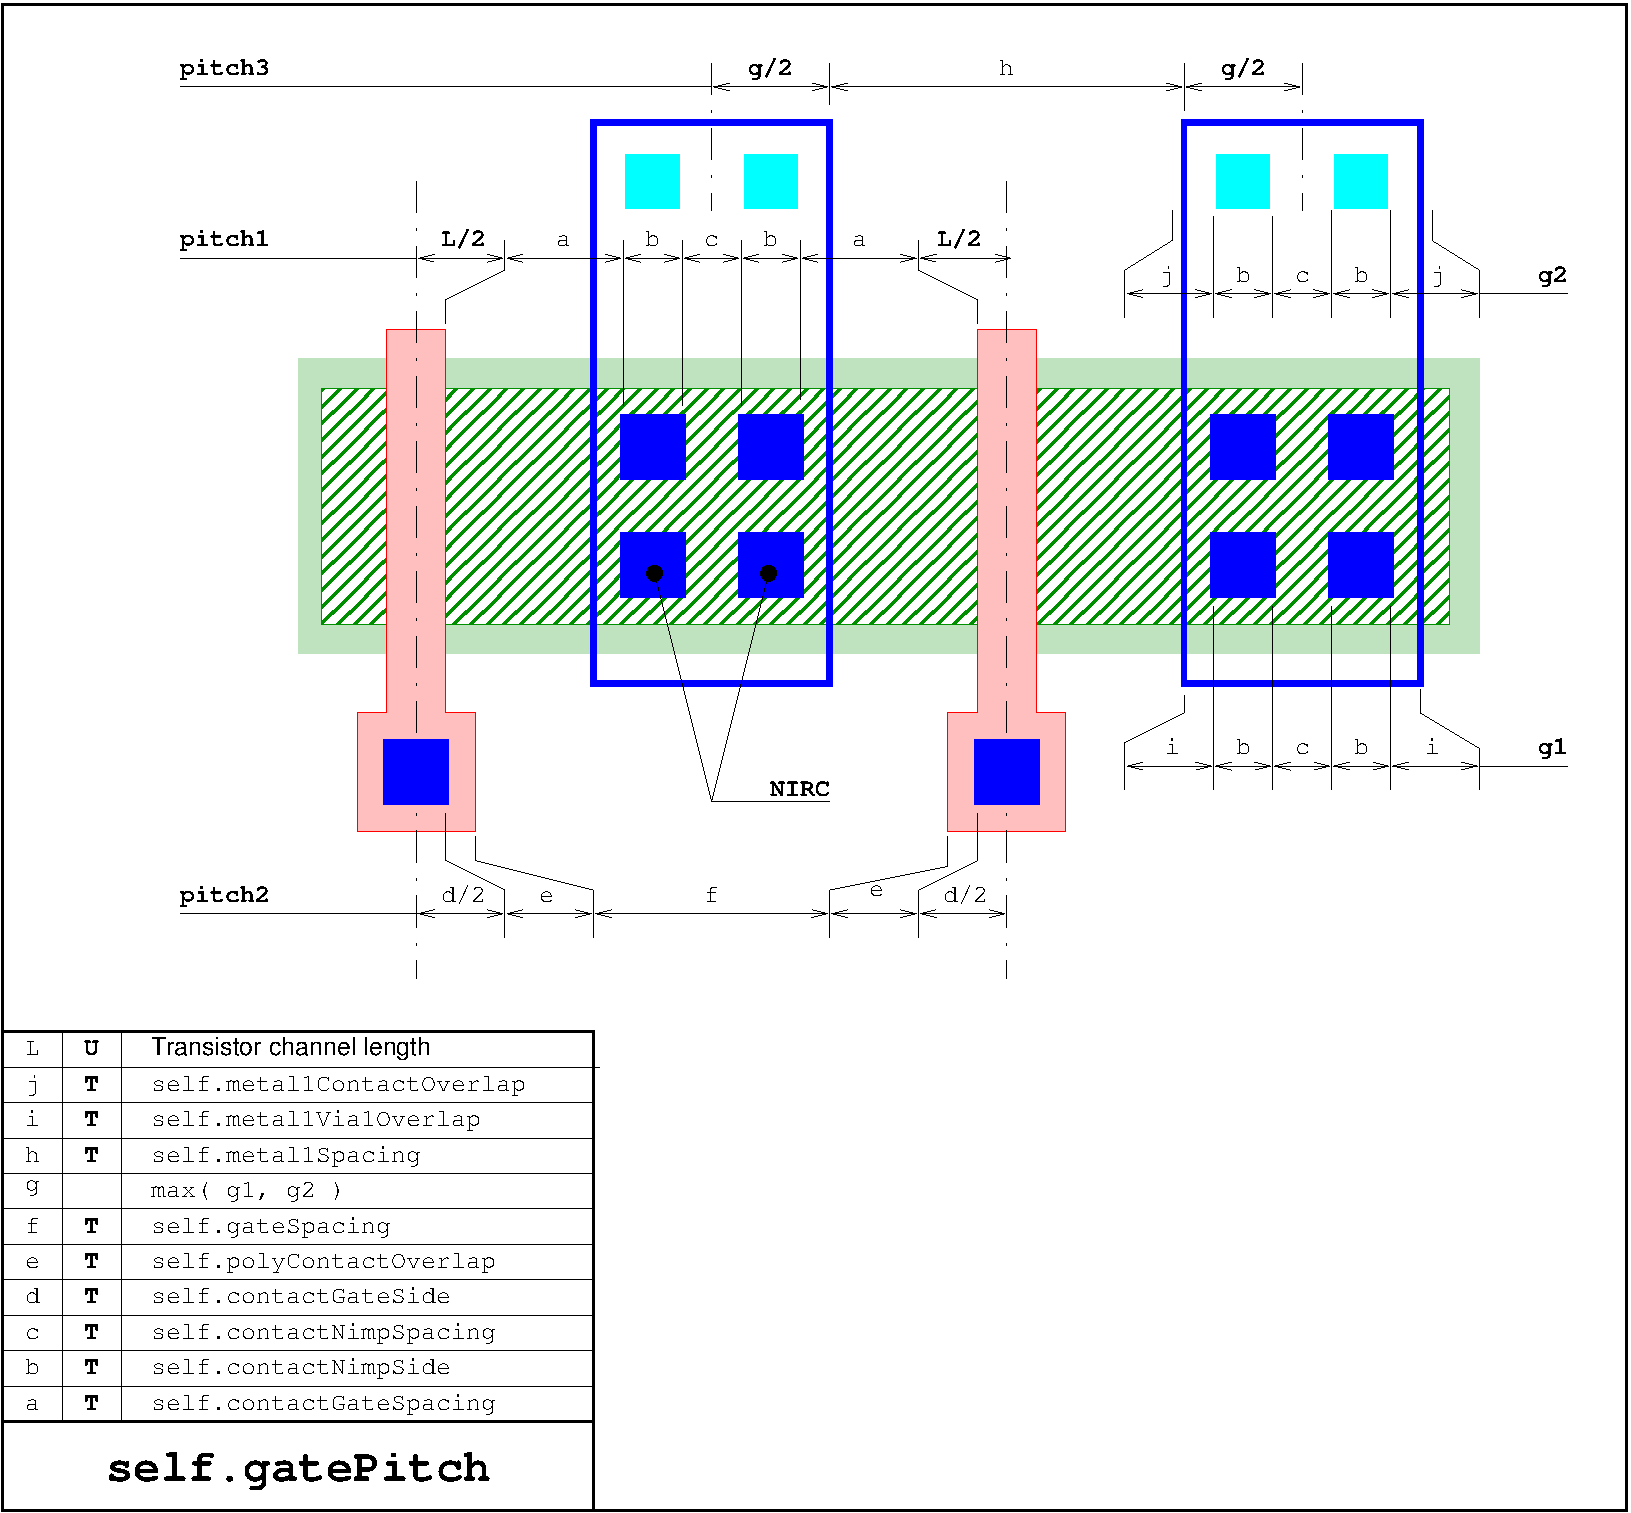
\includegraphics[width=.9\linewidth]{gate-pitch-1}
\caption{Gate Pitch}
\end{DoxyImage}
\hypertarget{classpython_1_1Stack_1_1Stack_secActiveSideWidth}{}\subsubsection{Active Side Width}\label{classpython_1_1Stack_1_1Stack_secActiveSideWidth}

\begin{DoxyItemize}
\item {\ttfamily self.\-active\-Side\-Width} \-: the distance between the axis of the last transistor gate (on the left or right) and the edge of the active area ({\itshape not} the diffusion area).
\end{DoxyItemize}

 
\begin{DoxyImage}
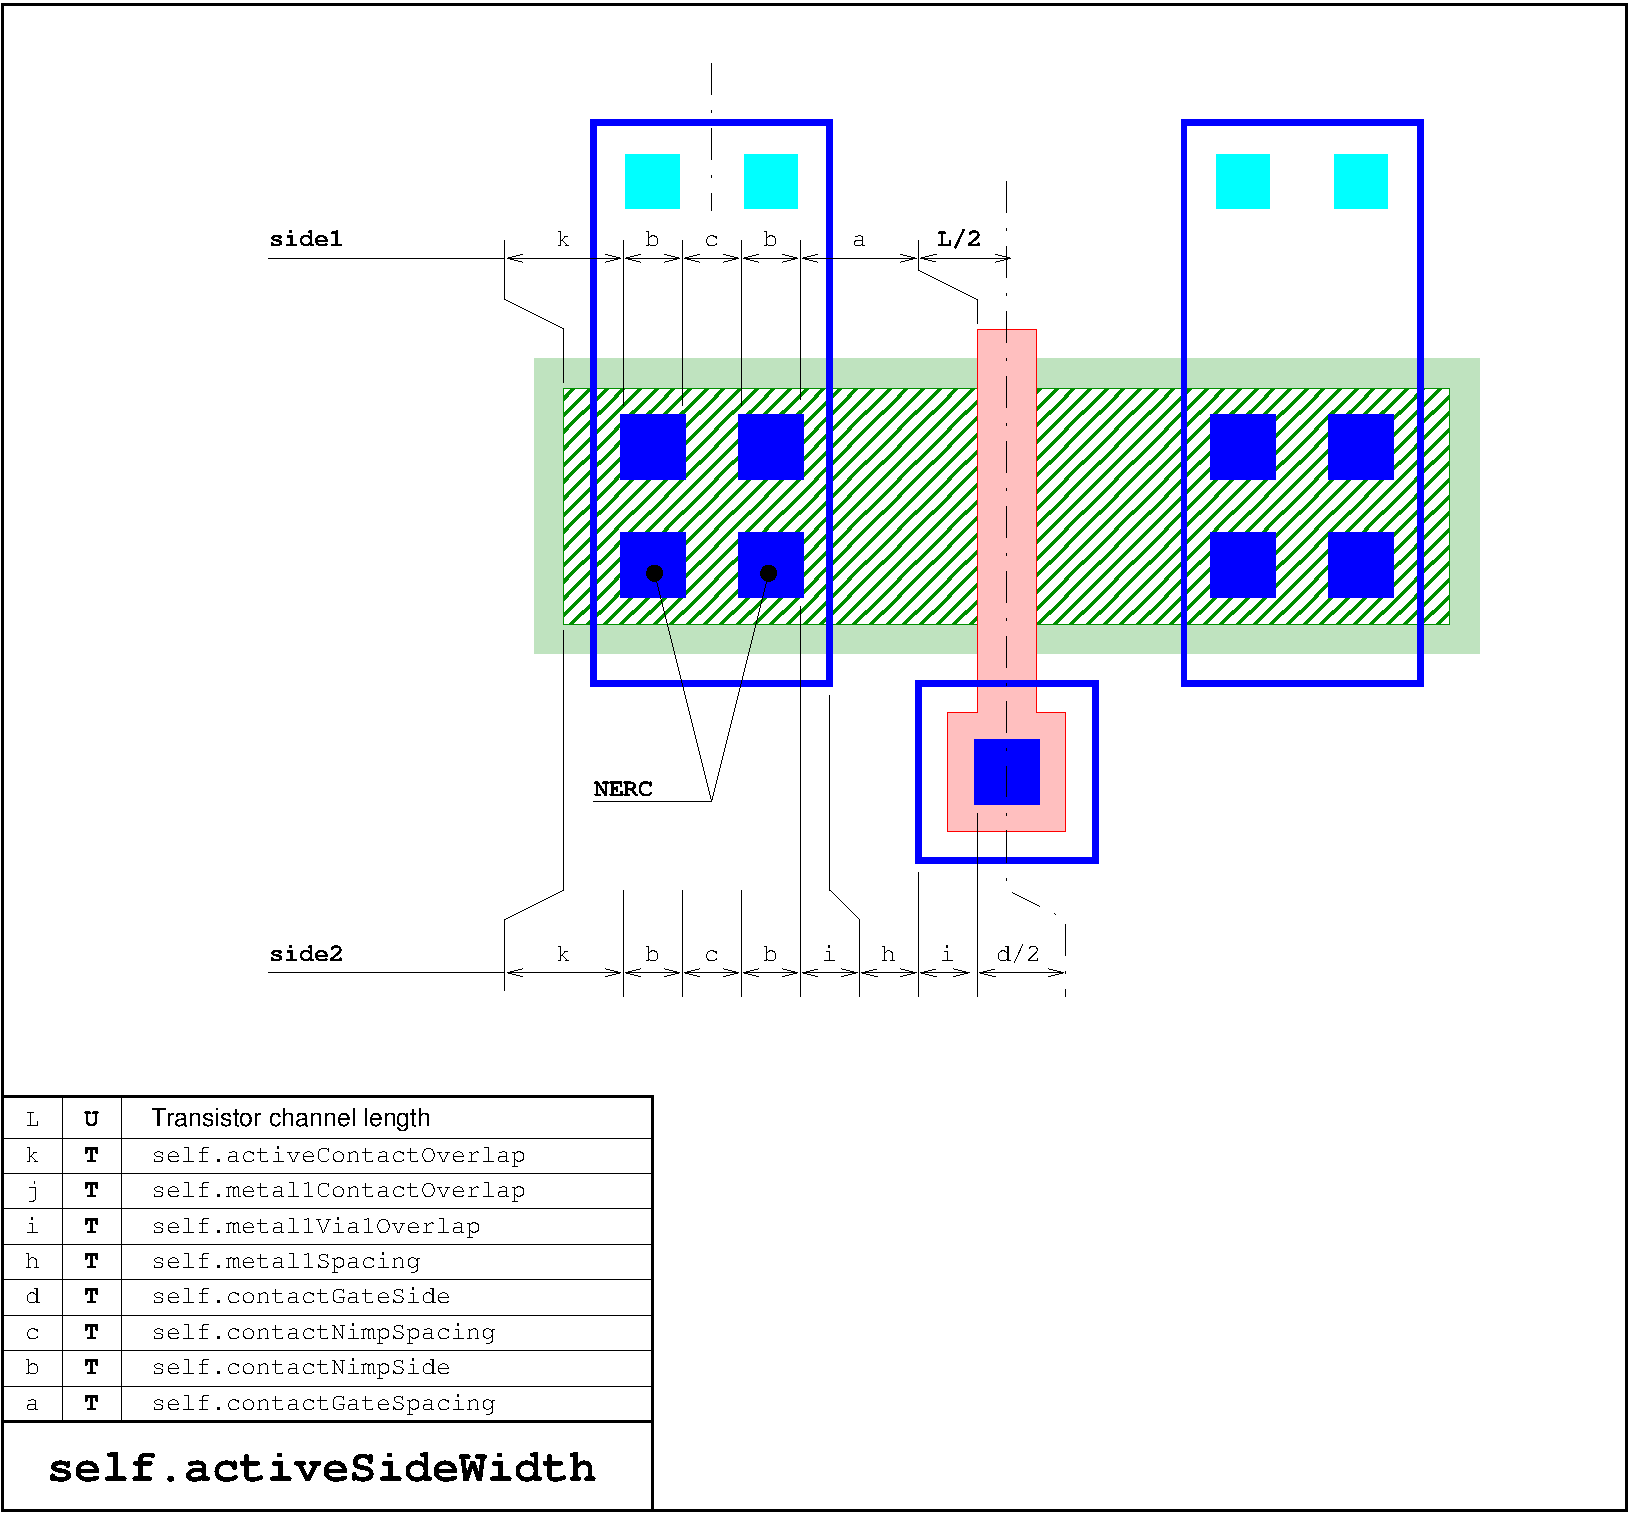
\includegraphics[width=.9\linewidth]{active-side-width-1}
\caption{Active Side Width}
\end{DoxyImage}
\hypertarget{classpython_1_1Stack_1_1Stack_secHTrackDistance}{}\subsubsection{H-\/\-Track Distance}\label{classpython_1_1Stack_1_1Stack_secHTrackDistance}

\begin{DoxyItemize}
\item {\ttfamily self.\-h\-Track\-Distance} \-: the minimal distance between either the top or bottom edge of the active area and the {\itshape axis} of the first track.
\end{DoxyItemize}

 
\begin{DoxyImage}
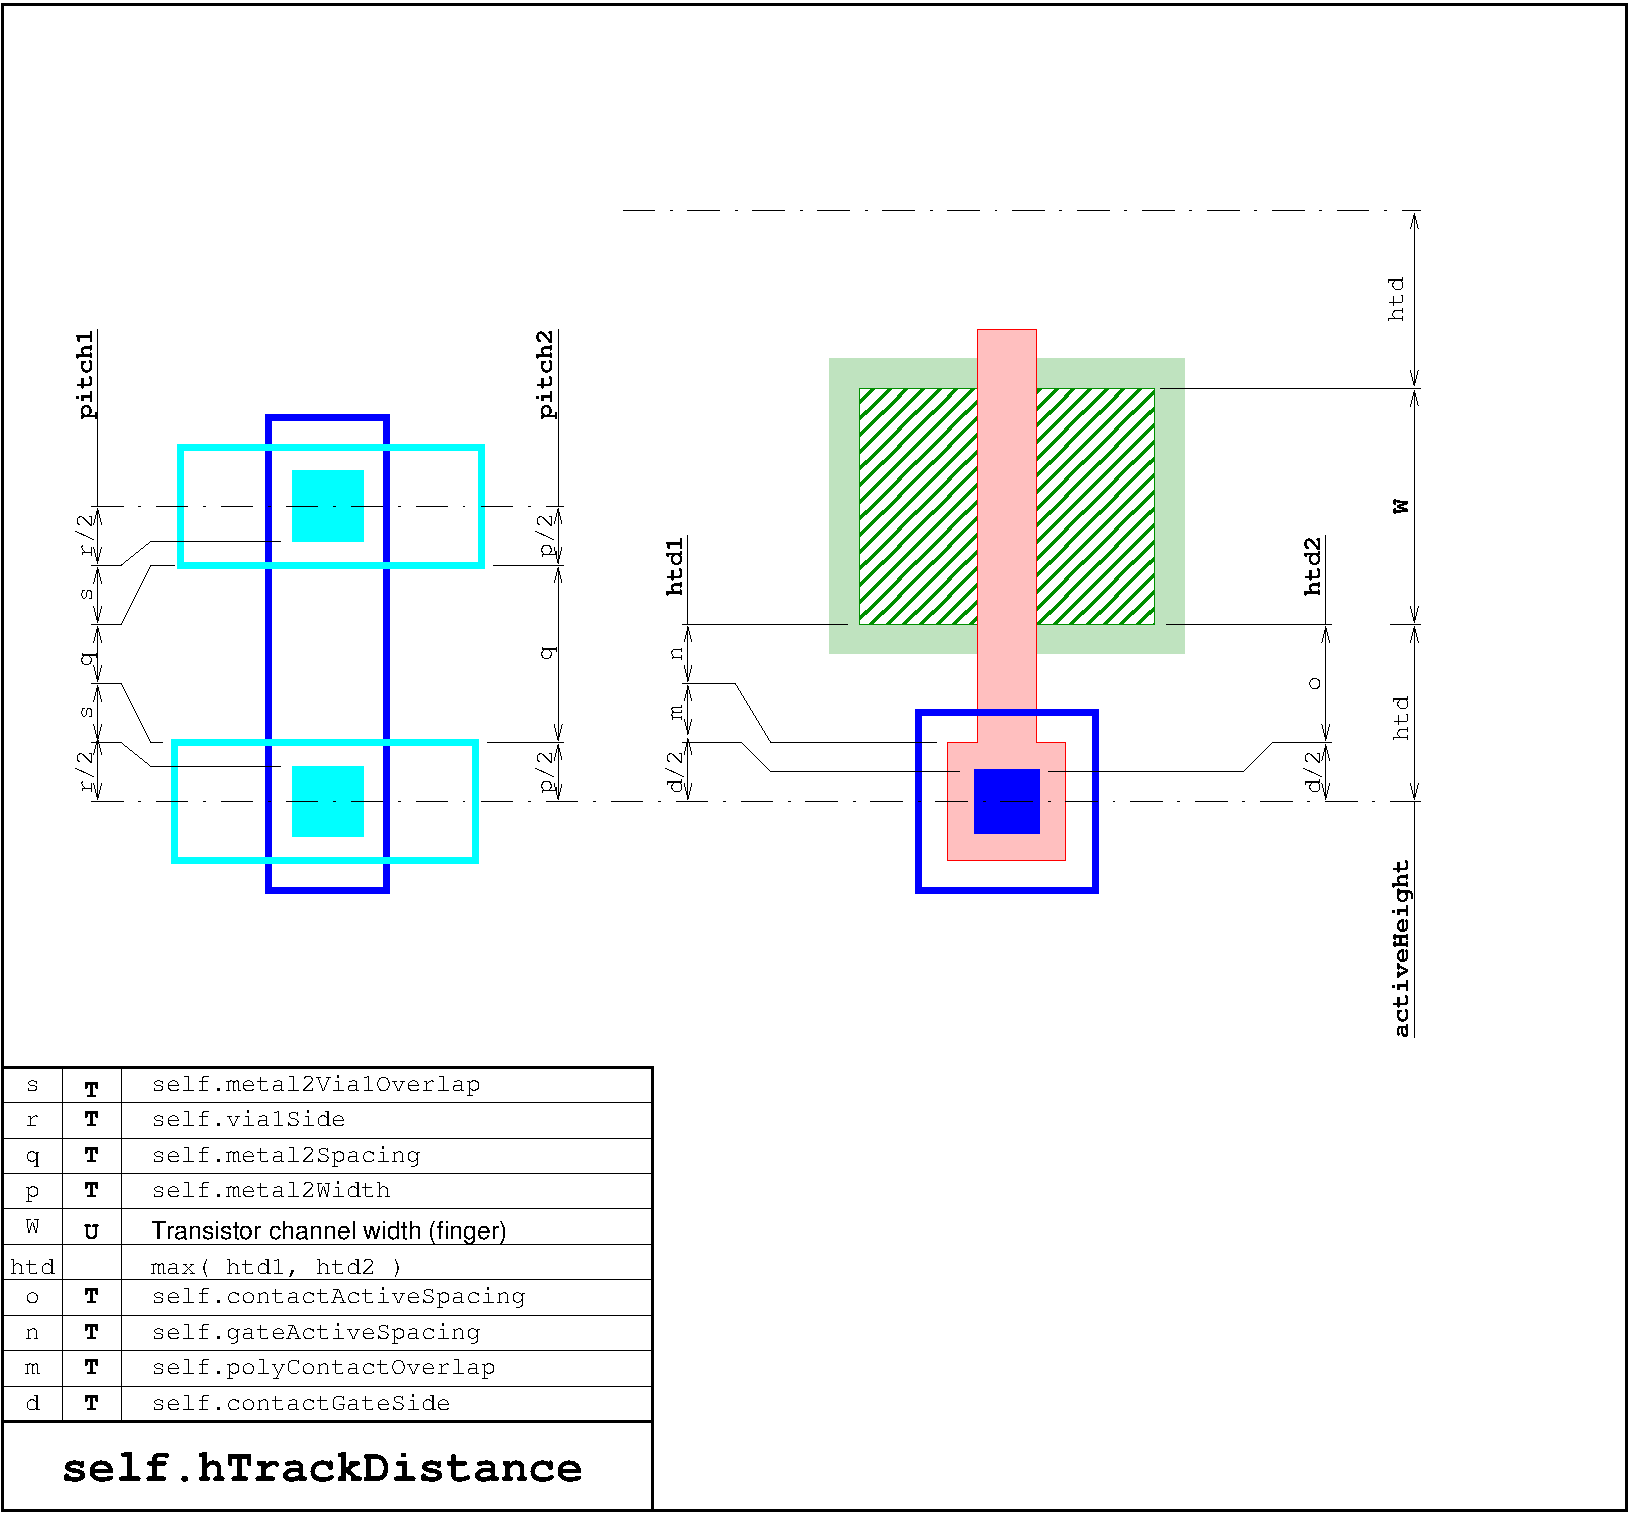
\includegraphics[width=.9\linewidth]{htrack-distance-1}
\caption{H-\/\-Track distance}
\end{DoxyImage}
\hypertarget{classpython_1_1Stack_1_1Stack_secOverallVariables}{}\subsubsection{Bounding\-Box \& Overall Variables}\label{classpython_1_1Stack_1_1Stack_secOverallVariables}

\begin{DoxyItemize}
\item {\ttfamily self.\-xpitches} \-: the number of vertical track pitches needed to fully enclose the active area.
\item {\ttfamily self.\-ypitches} \-: the number of horizontal track pitches needed to fully enclose the active area.
\item {\ttfamily self.\-active\-Offset\-X} \& {\ttfamily self.\-active\-Offset\-Y} \-: the offsets of the active area from the bottom left corner of the abutment box.
\item {\ttfamily self.\-diffusion\-Width} \& {\ttfamily self.\-diffusion\-Height} are the minimun dimensions required to fit the active area.
\item {\ttfamily self.\-top\-Tracks\-Nb()} \-: the number of tracks at the top of the stack.
\item {\ttfamily self.\-bot\-Tracks\-Nb()} \-: the number of tracks at the bottom of the stack.
\end{DoxyItemize}

 
\begin{DoxyImage}
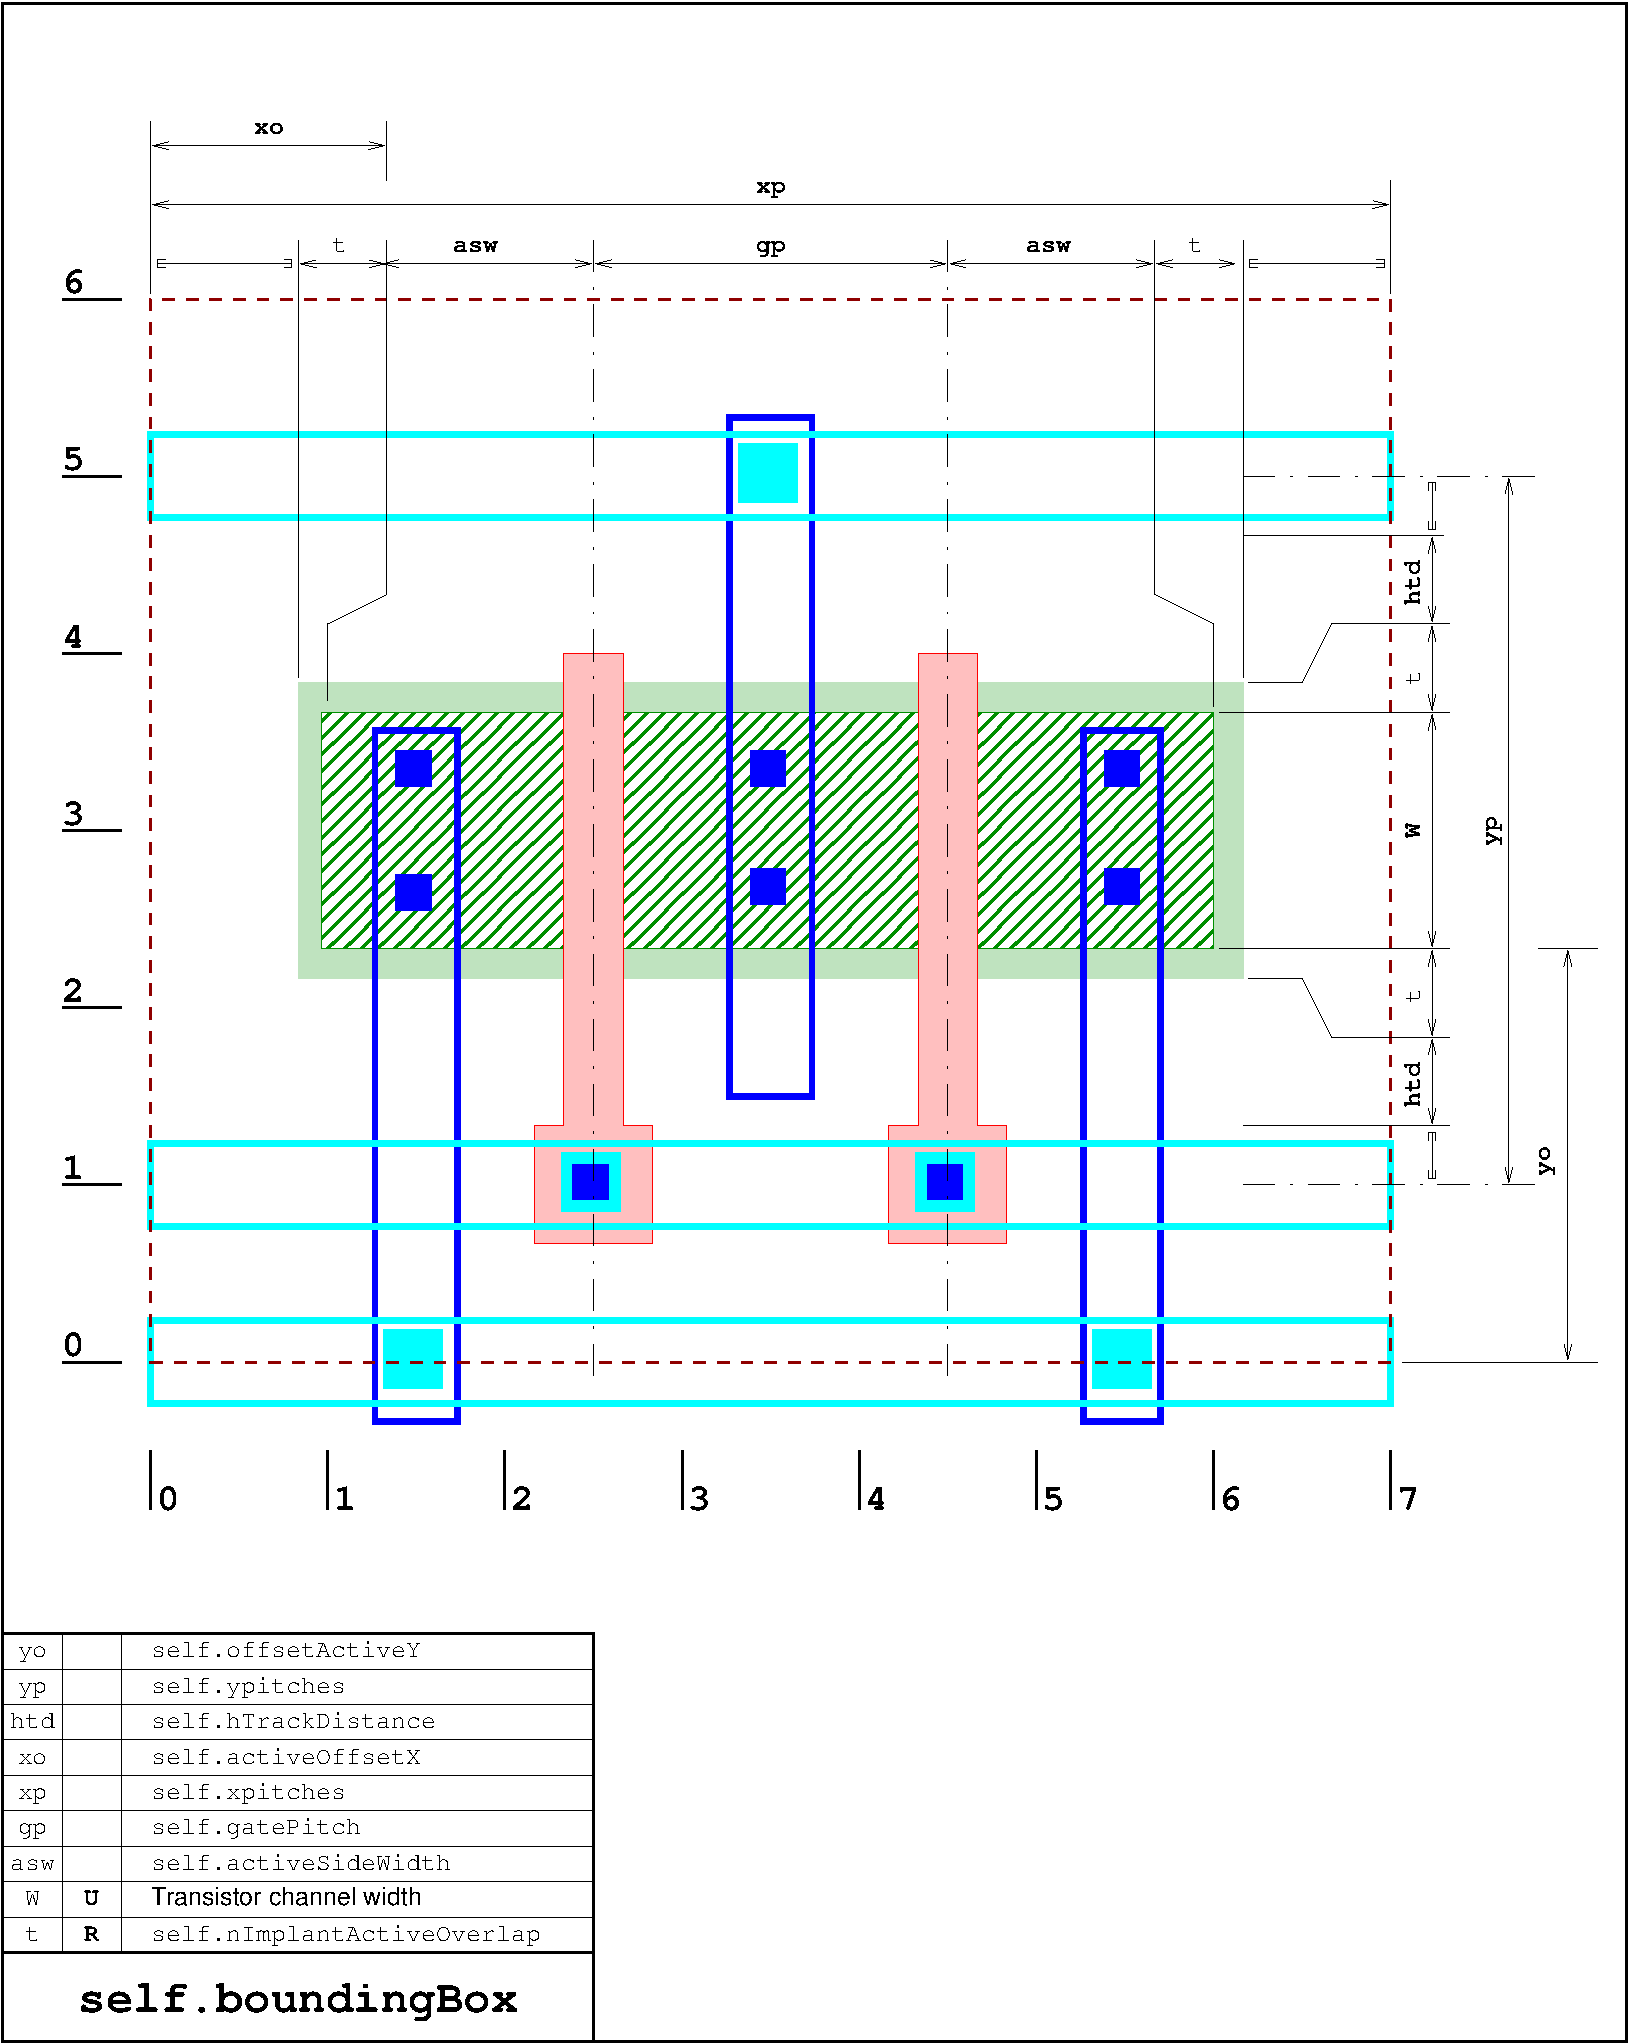
\includegraphics[width=.9\linewidth]{stack-layout-3}
\caption{General Stack Layout}
\end{DoxyImage}
\hypertarget{classpython_1_1Stack_1_1Stack_secWiringSpecs}{}\subsection{Wiring Specifications}\label{classpython_1_1Stack_1_1Stack_secWiringSpecs}
\hyperlink{classpython_1_1Stack_1_1Stack}{Stack} routing is done through vertical {\ttfamily metal1} wires coming from the gates and diffusions areas and {\ttfamily metal2} horizontal wires that can be either above or below the active area. {\ttfamily metal2} wires (or track) goes through the whole stack and are assigned to one net only. A net will have at least one track above or below and may have both.

The connections to the diffusions areas and gates of the various fingers are specified through a list. The stack is made of a regular alternation of diffusions and gates. The list tells, for each one starting from the left, to which net and track they are connected. For a stack of $NFs$ transistor fingers, the must wiring specification must contains $ 3 + (NFs-1) \times 2$ elements. The list is given through one {\itshape string} with each elements separated by one or more whitespace. The syntax for {\itshape one} element is detailed \hyperlink{classpython_1_1Stack_1_1Stack_secAtomicWiring}{Atomic Wiring Specification}.

{\bfseries Track numbering scheme}

Tracks above (top) the active area and below (bottom) each have their own numbering. In both case, the count start {\itshape from} the active area. This, the top tracks will be numbered by increasing Y and the bottom tracks by {\itshape decreasing} Y.

{\bfseries Track/\-Net assignement}

The track/net assignement is deduced from the atomic wiring specifications. It also allows to compute the total number of tracks needed above and below the active area.

 
\begin{DoxyImage}
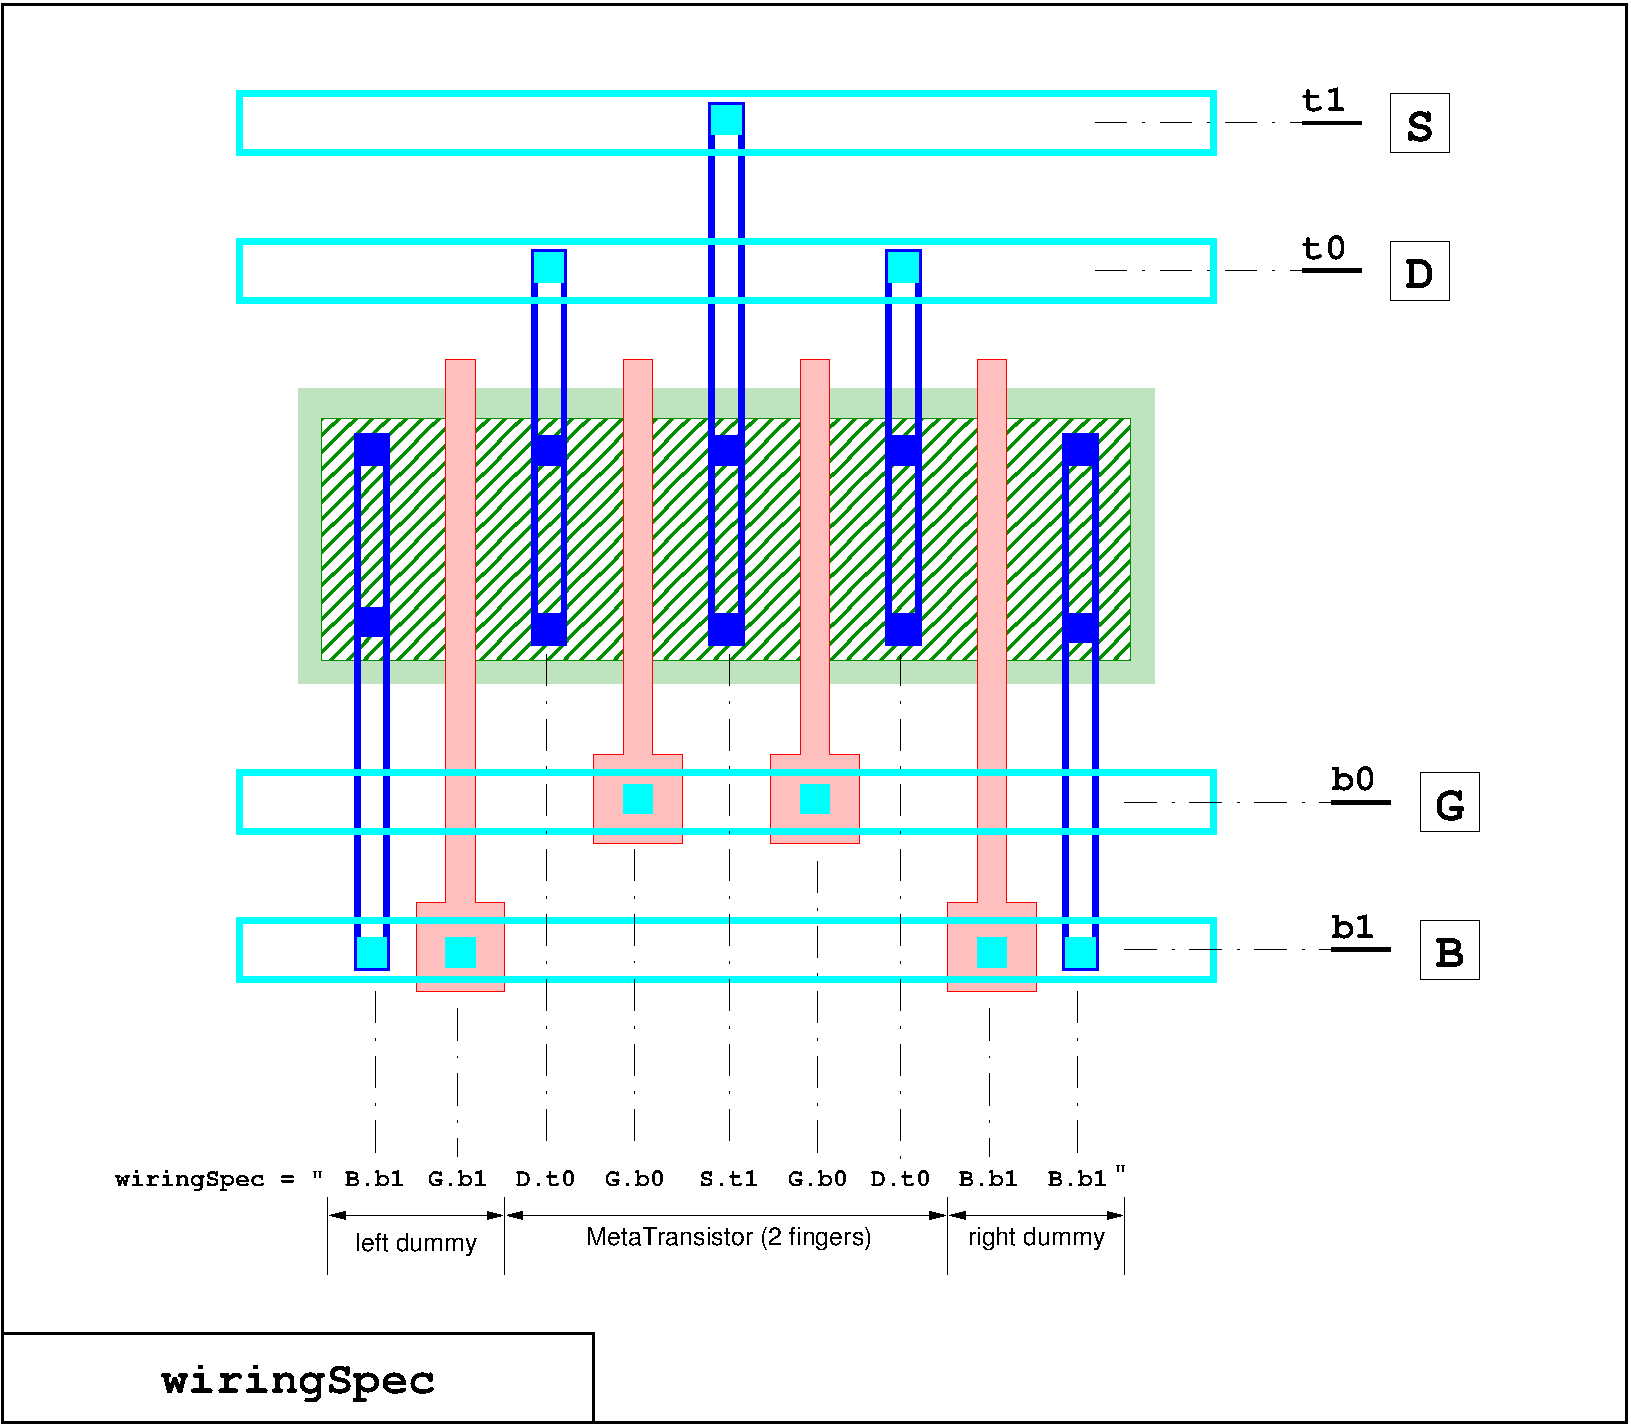
\includegraphics[width=.9\linewidth]{wiring-spec-2}
\caption{Wiring Specification}
\end{DoxyImage}
\hypertarget{classpython_1_1Stack_1_1Stack_secAtomicWiring}{}\subsubsection{Atomic Wiring Specification}\label{classpython_1_1Stack_1_1Stack_secAtomicWiring}
An atomic wiring specification has the same syntax for either diffusions or gates. It {\itshape must} not comprise any whitespaces. it is made of the following parts\-:
\begin{DoxyItemize}
\item The net name to connect to.
\item Whether the track is above the active area ({\ttfamily \char`\"{}t\char`\"{}}) or below ({\ttfamily \char`\"{}b\char`\"{}}). The special case ({\ttfamily \char`\"{}z\char`\"{}}) means that this element must be left unconnected (is such case possible?).
\item The number of the track.
\end{DoxyItemize}

 
\begin{DoxyImage}
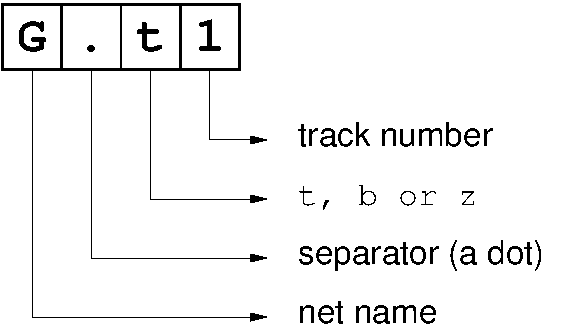
\includegraphics[width=.4\linewidth]{wiring-spec-1}
\caption{Atomic Wiring Specification}
\end{DoxyImage}
\hypertarget{classpython_1_1Stack_1_1Stack_secStackImplDetails}{}\subsection{Stack Implementation Details}\label{classpython_1_1Stack_1_1Stack_secStackImplDetails}
The {\ttfamily \-\_\-\-\_\-setattr\-\_\-\-\_\-()} and {\ttfamily \-\_\-\-\_\-getattr\-\_\-\-\_\-} functions have been redefined so that the technological values (rules) can be accessed has normal attributes of the \hyperlink{classpython_1_1Stack_1_1Stack}{Stack} class, in addition to the regular ones. 

\subsection{Constructor \& Destructor Documentation}
\hypertarget{classpython_1_1Stack_1_1Stack_ac775ee34451fdfa742b318538164070e}{\index{python\-::\-Stack\-::\-Stack@{python\-::\-Stack\-::\-Stack}!\-\_\-\-\_\-init\-\_\-\-\_\-@{\-\_\-\-\_\-init\-\_\-\-\_\-}}
\index{\-\_\-\-\_\-init\-\_\-\-\_\-@{\-\_\-\-\_\-init\-\_\-\-\_\-}!python::Stack::Stack@{python\-::\-Stack\-::\-Stack}}
\subsubsection[{\-\_\-\-\_\-init\-\_\-\-\_\-}]{\setlength{\rightskip}{0pt plus 5cm}def \-\_\-\-\_\-init\-\_\-\-\_\- (
\begin{DoxyParamCaption}
\item[{}]{self, }
\item[{}]{device, }
\item[{}]{N\-E\-R\-C, }
\item[{}]{N\-I\-R\-C}
\end{DoxyParamCaption}
)}}\label{classpython_1_1Stack_1_1Stack_ac775ee34451fdfa742b318538164070e}


{\bfseries \mbox{[}A\-P\-I\mbox{]}} Constructor 

param rules The physical rule set. 
\begin{DoxyParams}{Parameters}
{\em device} & The {\bf Hurricane} A\-M\-S device into which the layout will be drawn. \\
\hline
{\em N\-E\-R\-C} & Number of contact rows in external (first \& last) diffusion connectors. \\
\hline
{\em N\-I\-R\-C} & Number of contact rows in middle diffusion connectors. param w The {\bfseries width} of every transistor of the stack (aka {\itshape fingers}). param L The {\bfseries length} of every transistor. param N\-Fs The total number of fingers (dummies includeds). param N\-Ds The number of dummies to put on each side of the stack. \\
\hline
\end{DoxyParams}


References Stack.\-b\-Implant\-Layer, Stack.\-bot\-Tracks, Stack.\-bot\-W\-Tracks, Stack.\-bulk\-Net, Stack.\-bulks, Stack.\-device, Stack.\-dimensioned, Bulk.\-flags, Stack.\-flags, Stack.\-is\-Nmos(), Stack.\-L, Stack.\-meta\-Tnb(), Stack.\-meta\-Transistors, Stack.\-N\-Ds, Stack.\-N\-E\-R\-C, Stack.\-N\-Fs, Stack.\-N\-I\-R\-C, Stack.\-t\-Implant\-Layer, Stack.\-top\-Tracks, Stack.\-top\-W\-Tracks, Stack.\-w, Stack.\-well\-Layer, and Stack.\-wirings.



\subsection{Member Function Documentation}
\hypertarget{classpython_1_1Stack_1_1Stack_ad7f0300aaad3ad8b2de70ae6c106c102}{\index{python\-::\-Stack\-::\-Stack@{python\-::\-Stack\-::\-Stack}!set\-Wirings@{set\-Wirings}}
\index{set\-Wirings@{set\-Wirings}!python::Stack::Stack@{python\-::\-Stack\-::\-Stack}}
\subsubsection[{set\-Wirings}]{\setlength{\rightskip}{0pt plus 5cm}def set\-Wirings (
\begin{DoxyParamCaption}
\item[{}]{self, }
\item[{}]{wiring\-Spec}
\end{DoxyParamCaption}
)}}\label{classpython_1_1Stack_1_1Stack_ad7f0300aaad3ad8b2de70ae6c106c102}


{\bfseries \mbox{[}A\-P\-I\mbox{]}} Set the \hyperlink{classpython_1_1Stack_1_1Stack}{Stack} wiring specification. 


\begin{DoxyParams}{Parameters}
{\em wiring\-Spec} & A string defining the connections for the gates and diffusion areas.\\
\hline
\end{DoxyParams}
For a comprehensive explanation of the wiring specification, refers to \hyperlink{classpython_1_1Stack_1_1Stack_secWiringSpecs}{Wiring Specifications} . 

References Stack.\-bot\-Tracks, Stack.\-bot\-Tracks\-Nb(), Stack.\-bot\-W\-Tracks, Stack.\-bulk\-Net, Stack.\-compute\-Dimensions(), Stack.\-device, Stack.\-dimensioned, Stack.\-e\-Diff\-Metal1\-Width, Bulk.\-flags, Stack.\-flags, Stack.\-gate\-Pitch, Stack.\-get\-Bot\-Track\-Y(), Stack.\-get\-Horizontal\-Width(), Stack.\-hor\-Pitch, Stack.\-L, Stack.\-metal1\-To\-Gate, Stack.\-meta\-Transistors, Stack.\-side\-Active\-Width, Stack.\-top\-Tracks, Stack.\-top\-Tracks\-Nb(), Stack.\-top\-W\-Tracks, Stack.\-wirings, and Stack.\-ypitches.

\hypertarget{classpython_1_1Stack_1_1Stack_a20b46b43488cc58c302b123a89299d85}{\index{python\-::\-Stack\-::\-Stack@{python\-::\-Stack\-::\-Stack}!compute\-Dimensions@{compute\-Dimensions}}
\index{compute\-Dimensions@{compute\-Dimensions}!python::Stack::Stack@{python\-::\-Stack\-::\-Stack}}
\subsubsection[{compute\-Dimensions}]{\setlength{\rightskip}{0pt plus 5cm}def compute\-Dimensions (
\begin{DoxyParamCaption}
\item[{}]{self}
\end{DoxyParamCaption}
)}}\label{classpython_1_1Stack_1_1Stack_a20b46b43488cc58c302b123a89299d85}


{\bfseries \mbox{[}internal\mbox{]}} Compute \hyperlink{classpython_1_1Stack_1_1Stack}{Stack} dimensions from the technological rules. 

{\bfseries Internal function.} Perform the computation of\-:
\begin{DoxyItemize}
\item {\ttfamily self.\-metal1\-Pitch} 
\item {\ttfamily self.\-min\-Width\-\_\-metal1} 
\item {\ttfamily self.\-metal2\-Pitch} 
\item {\ttfamily self.\-min\-Width\-\_\-metal2} 
\item {\ttfamily self.\-gate\-Pitch} 
\item {\ttfamily self.\-side\-Active\-Width} 
\item {\ttfamily self.\-h\-Track\-Distance} 
\item {\ttfamily self.\-xpitches} 
\item {\ttfamily self.\-ypitches} 
\item {\ttfamily self.\-active\-Offset\-X} 
\item {\ttfamily self.\-active\-Offset\-Y} 
\item {\ttfamily self.\-bounding\-Box} 
\end{DoxyItemize}

References Stack.\-active\-Box, Stack.\-active\-Offset\-X, Stack.\-active\-Offset\-Y, Stack.\-bb\-Height, Stack.\-bb\-Width, Stack.\-bot\-W\-Tracks, Stack.\-bounding\-Box, Stack.\-bulks, Stack.\-bulk\-Width, Stack.\-compute\-Layout\-Parasitics(), Stack.\-compute\-Stress\-Effect(), Stack.\-contact\-Diff\-Pitch, Stack.\-contact\-Diff\-Side, Stack.\-D\-G\-G, Stack.\-D\-G\-I, Stack.\-dimensioned, Stack.\-D\-M\-C\-G, Stack.\-D\-M\-C\-G\-T, Stack.\-D\-M\-C\-I, Stack.\-e\-Diff\-Metal1\-Width, Bulk.\-flags, Stack.\-flags, Stack.\-gate\-Pitch, Stack.\-gate\-Via1\-Pitch, Stack.\-get\-Bot\-Track\-Y(), Stack.\-get\-Horizontal\-Width(), Stack.\-get\-Last\-Top\-Track\-Y(), Stack.\-hor\-Pitch, Stack.\-h\-Track\-Distance, Stack.\-i\-Diff\-Metal1\-Width, Stack.\-is\-V\-H, Stack.\-L, Stack.\-metal1\-To\-Gate, Stack.\-metal2\-Pitch, Stack.\-metal2\-Techno\-Pitch, Stack.\-metal3\-Pitch, Stack.\-N\-E\-R\-C, Stack.\-N\-Fs, Stack.\-N\-I\-R\-C, Stack.\-side\-Active\-Width, Stack.\-tracks\-Nb\-Pitch(), Stack.\-v\-Bulk\-Distance, Stack.\-ver\-Pitch, Stack.\-w, Stack.\-wire1\-Width, Stack.\-wire2\-Width, Stack.\-wire3\-Width, Stack.\-wirings, Stack.\-xpitches, and Stack.\-ypitches.



Referenced by Capacitor\-Unit.\-create(), Stack.\-do\-Layout(), Rout\-Matched\-Capacitor.\-route(), and Stack.\-set\-Wirings().

\hypertarget{classpython_1_1Stack_1_1Stack_affc52c42a8c72dc1125ddce55647a6f9}{\index{python\-::\-Stack\-::\-Stack@{python\-::\-Stack\-::\-Stack}!do\-Layout@{do\-Layout}}
\index{do\-Layout@{do\-Layout}!python::Stack::Stack@{python\-::\-Stack\-::\-Stack}}
\subsubsection[{do\-Layout}]{\setlength{\rightskip}{0pt plus 5cm}def do\-Layout (
\begin{DoxyParamCaption}
\item[{}]{self, }
\item[{}]{bb\-Mode}
\end{DoxyParamCaption}
)}}\label{classpython_1_1Stack_1_1Stack_affc52c42a8c72dc1125ddce55647a6f9}


{\bfseries \mbox{[}A\-P\-I\mbox{]}} Draw the complete layout. 

Draw the commplete layout of the \hyperlink{classpython_1_1Stack_1_1Stack}{Stack}. 

References Stack.\-active\-Offset\-X, Stack.\-active\-Offset\-Y, Stack.\-bb\-Width, Stack.\-bot\-Tracks, Stack.\-bot\-W\-Tracks, Stack.\-bounding\-Box, Stack.\-bulk\-Net, Stack.\-bulks, Stack.\-bulk\-Width, Stack.\-compute\-Dimensions(), Stack.\-contact\-Diff\-Pitch, Stack.\-device, Stack.\-D\-G\-G, Stack.\-D\-G\-I, Stack.\-D\-M\-C\-G, Stack.\-D\-M\-C\-G\-T, Stack.\-D\-M\-C\-I, Stack.\-draw\-Active(), Stack.\-draw\-Gate(), Stack.\-draw\-Source\-Drain(), Stack.\-draw\-Well(), Stack.\-e\-Diff\-Metal1\-Width, Bulk.\-flags, Stack.\-flags, Stack.\-gate\-Pitch, Stack.\-gate\-Via1\-Pitch, Stack.\-get\-Bot\-Track\-Y(), Stack.\-get\-Horizontal\-Axis(), Stack.\-get\-Horizontal\-Width(), Stack.\-get\-Top\-Track\-Y(), Stack.\-get\-Wiring\-Width(), Stack.\-hor\-Pitch, Stack.\-i\-Diff\-Metal1\-Width, Stack.\-is\-Bot\-Track(), Stack.\-is\-V\-H, Stack.\-L, Stack.\-metal1\-To\-Gate, Stack.\-N\-E\-R\-C, Stack.\-N\-Fs, Stack.\-N\-I\-R\-C, Stack.\-side\-Active\-Width, Stack.\-t\-Implant\-Layer, Stack.\-top\-Tracks, Stack.\-top\-W\-Tracks, Stack.\-w, Stack.\-well\-Layer, Stack.\-wire1\-Width, Stack.\-wire2\-Width, Stack.\-wire3\-Width, and Stack.\-wirings.



The documentation for this class was generated from the following file\-:\begin{DoxyCompactItemize}
\item 
Stack.\-py\end{DoxyCompactItemize}

\hypertarget{classpython_1_1CapacitorVRTracks_1_1VerticalRoutingTracks}{\section{Vertical\-Routing\-Tracks Class Reference}
\label{classpython_1_1CapacitorVRTracks_1_1VerticalRoutingTracks}\index{Vertical\-Routing\-Tracks@{Vertical\-Routing\-Tracks}}
}


Route two matched capacitors, C1 and C2, drawn in a capacitor matrix.  




Inherits Capacitor\-Unit, and Capacitor\-Stack.

\subsection*{Public Member Functions}
\begin{DoxyCompactItemize}
\item 
def \hyperlink{classpython_1_1CapacitorVRTracks_1_1VerticalRoutingTracks_a42e286a4157e638ddb3d96ce7c47dece}{\-\_\-\-\_\-set\-Stretching\-\_\-\-\_\-}
\begin{DoxyCompactList}\small\item\em Sets vertical stretching value considering spacing between elementary capacitors in the matrix. \end{DoxyCompactList}\item 
def \hyperlink{classpython_1_1CapacitorVRTracks_1_1VerticalRoutingTracks_a3b578035b1559391931dade7c2508105}{set\-Rules}
\begin{DoxyCompactList}\small\item\em Defines technology rules used to draw the layout. \end{DoxyCompactList}\item 
def \hyperlink{classpython_1_1CapacitorVRTracks_1_1VerticalRoutingTracks_ab509e7c1cfbf2826e4418a606c8982a3}{draw\-V\-Routing\-Tracks}
\begin{DoxyCompactList}\small\item\em Iteratively draws vertical routing tracks given the physical layer {\ttfamily v\-Routing\-Tracks\-Layer}. \end{DoxyCompactList}\end{DoxyCompactItemize}


\subsection{Detailed Description}
Route two matched capacitors, C1 and C2, drawn in a capacitor matrix. 

Connections are put in place with reference to a given matching scheme. Elementary capacitor units are connected to horizontal and vertical routing tracks that represent top plates and bottom plates nets of C1 and C2. Supported types of capacitors are Poly-\/\-Poly and Metal-\/\-Metal. Technologycal rules are provided by 350 nm A\-M\-S C\-M\-O\-S technology with three-\/four metal layers. Metal layers that are used for routeing are placed similarly to horziontal-\/vertical (H\-V) symbolic Alliance C\-A\-D tool router, where horizontal metal channels are drawn in metal 2 and the vertical ones are in metal 3. Given a matrix of dimensions $ R*C $, the total number of vertical tracks is $ 2C+2 $ equivalent to $ C+1 $ couples, ensuring that every elementary capacitor is positioned between four vertical tracks, two from each side. In fact, every adjacent couple of these tracks represent top plates and bottom plates of C1 or C2 as shown in Figure 1.



An elementary capacitor unit can be a part of C1 or C2 according to the matching scheme. However, to respect common-\/centroid layout specifications, for C1 and C2 to be equal, the matrix number of colums and number of rows must be both even. Addionnally, the number of elementary capacitors dedicated to C1 must be equal to those dedicated to C2. These two conditions are tested in one of the class methods. An exception is raised if at least one of the two is not respected. 

\subsection{Member Function Documentation}
\hypertarget{classpython_1_1CapacitorVRTracks_1_1VerticalRoutingTracks_a42e286a4157e638ddb3d96ce7c47dece}{\index{python\-::\-Capacitor\-V\-R\-Tracks\-::\-Vertical\-Routing\-Tracks@{python\-::\-Capacitor\-V\-R\-Tracks\-::\-Vertical\-Routing\-Tracks}!\-\_\-\-\_\-set\-Stretching\-\_\-\-\_\-@{\-\_\-\-\_\-set\-Stretching\-\_\-\-\_\-}}
\index{\-\_\-\-\_\-set\-Stretching\-\_\-\-\_\-@{\-\_\-\-\_\-set\-Stretching\-\_\-\-\_\-}!python::CapacitorVRTracks::VerticalRoutingTracks@{python\-::\-Capacitor\-V\-R\-Tracks\-::\-Vertical\-Routing\-Tracks}}
\subsubsection[{\-\_\-\-\_\-set\-Stretching\-\_\-\-\_\-}]{\setlength{\rightskip}{0pt plus 5cm}def \-\_\-\-\_\-set\-Stretching\-\_\-\-\_\- (
\begin{DoxyParamCaption}
\item[{}]{self}
\end{DoxyParamCaption}
)}}\label{classpython_1_1CapacitorVRTracks_1_1VerticalRoutingTracks_a42e286a4157e638ddb3d96ce7c47dece}


Sets vertical stretching value considering spacing between elementary capacitors in the matrix. 

\begin{DoxyReturn}{Returns}
stratching value. 
\end{DoxyReturn}


References Vertical\-Routing\-Tracks.\-abutment\-Box\-\_\-spacing, Capacitor\-Stack.\-abutment\-Box\-\_\-spacing, and Rout\-Matched\-Capacitor.\-abutment\-Box\-\_\-spacing.



Referenced by Rout\-Matched\-Capacitor.\-compute\-H\-R\-Layer\-Y\-Center(), and Vertical\-Routing\-Tracks.\-draw\-V\-Routing\-Tracks().

\hypertarget{classpython_1_1CapacitorVRTracks_1_1VerticalRoutingTracks_a3b578035b1559391931dade7c2508105}{\index{python\-::\-Capacitor\-V\-R\-Tracks\-::\-Vertical\-Routing\-Tracks@{python\-::\-Capacitor\-V\-R\-Tracks\-::\-Vertical\-Routing\-Tracks}!set\-Rules@{set\-Rules}}
\index{set\-Rules@{set\-Rules}!python::CapacitorVRTracks::VerticalRoutingTracks@{python\-::\-Capacitor\-V\-R\-Tracks\-::\-Vertical\-Routing\-Tracks}}
\subsubsection[{set\-Rules}]{\setlength{\rightskip}{0pt plus 5cm}def set\-Rules (
\begin{DoxyParamCaption}
\item[{}]{self}
\end{DoxyParamCaption}
)}}\label{classpython_1_1CapacitorVRTracks_1_1VerticalRoutingTracks_a3b578035b1559391931dade7c2508105}


Defines technology rules used to draw the layout. 

Some of the rules, namely those describing routeing layers and tracks are applicable for both M\-I\-M and P\-I\-P capacitors. However, cuts rules are different. \begin{DoxyParagraph}{Remark\-:}
All {\ttfamily Capacitor\-Stack} class rules are also reloaded in this class. An exception is raised if the entered capacitor type is unsupported. 
\end{DoxyParagraph}
\begin{DoxyReturn}{Returns}
a dictionary with rules labels as keys and rules content as values. 
\end{DoxyReturn}


References Vertical\-Routing\-Tracks.\-capacitors\-Number, Capacitor\-Stack.\-capacitors\-Number, Vertical\-Routing\-Tracks.\-compute\-V\-R\-T\-Dimensions(), Vertical\-Routing\-Tracks.\-draw\-V\-Routing\-Tracks(), Vertical\-Routing\-Tracks.\-min\-Enclosure\-\_\-h\-Routing\-Layer\-\_\-v\-Routing\-Track\-\_\-cut, Vertical\-Routing\-Tracks.\-min\-Enclosure\-\_\-h\-Routing\-Track\-Cut, Vertical\-Routing\-Tracks.\-minimize\-V\-R\-Ts(), Vertical\-Routing\-Tracks.\-min\-Spacing\-\_\-h\-Routing\-Track, Rout\-Matched\-Capacitor.\-min\-Spacing\-\_\-h\-Routing\-Track, Vertical\-Routing\-Tracks.\-min\-Width\-\_\-h\-Routing\-Layer, Vertical\-Routing\-Tracks.\-min\-Width\-\_\-h\-Routing\-Layer\-\_\-v\-Routing\-Track\-\_\-cut, Vertical\-Routing\-Tracks.\-min\-Width\-\_\-h\-Routing\-Track, Vertical\-Routing\-Tracks.\-min\-Width\-\_\-h\-Routing\-Track\-Cut, Vertical\-Routing\-Tracks.\-set\-Rules(), Capacitor\-Stack.\-set\-Rules(), Capacitor\-Unit.\-set\-Rules(), and Rout\-Matched\-Capacitor.\-set\-Rules().



Referenced by Vertical\-Routing\-Tracks.\-set\-Rules().

\hypertarget{classpython_1_1CapacitorVRTracks_1_1VerticalRoutingTracks_ab509e7c1cfbf2826e4418a606c8982a3}{\index{python\-::\-Capacitor\-V\-R\-Tracks\-::\-Vertical\-Routing\-Tracks@{python\-::\-Capacitor\-V\-R\-Tracks\-::\-Vertical\-Routing\-Tracks}!draw\-V\-Routing\-Tracks@{draw\-V\-Routing\-Tracks}}
\index{draw\-V\-Routing\-Tracks@{draw\-V\-Routing\-Tracks}!python::CapacitorVRTracks::VerticalRoutingTracks@{python\-::\-Capacitor\-V\-R\-Tracks\-::\-Vertical\-Routing\-Tracks}}
\subsubsection[{draw\-V\-Routing\-Tracks}]{\setlength{\rightskip}{0pt plus 5cm}def draw\-V\-Routing\-Tracks (
\begin{DoxyParamCaption}
\item[{}]{self, }
\item[{}]{v\-Routing\-Tracks\-Layer}
\end{DoxyParamCaption}
)}}\label{classpython_1_1CapacitorVRTracks_1_1VerticalRoutingTracks_ab509e7c1cfbf2826e4418a606c8982a3}


Iteratively draws vertical routing tracks given the physical layer {\ttfamily v\-Routing\-Tracks\-Layer}. 

Every elementary capacitor is consequently positioned between four routing tracks, two from each side. Each couple of adjacent routeing tracks represent top plate and bottom plate nets of Ci, where i is in \mbox{[}1,2\mbox{]}. As given in Figure 2, capacitor $ C_{ij} $ with an even j value situated in even columns have and inversely for odd columns numbers. 

References Vertical\-Routing\-Tracks.\-\_\-\-\_\-compute\-V\-R\-Ts\-Number\-\_\-\-\_\-(), Vertical\-Routing\-Tracks.\-\_\-\-\_\-find\-Cap\-Ids\-To\-Eliminate\-\_\-\-\_\-(), Vertical\-Routing\-Tracks.\-\_\-\-\_\-find\-Cap\-Ids\-To\-Eliminate\-Per\-Column\-\_\-\-\_\-(), Vertical\-Routing\-Tracks.\-\_\-\-\_\-find\-Used\-Cap\-Ids\-Per\-Column\-\_\-\-\_\-(), Vertical\-Routing\-Tracks.\-\_\-\-\_\-find\-V\-R\-Ts\-To\-Eliminate\-\_\-\-\_\-(), Vertical\-Routing\-Tracks.\-\_\-\-\_\-set\-Nets\-Distribution\-\_\-\-\_\-(), Vertical\-Routing\-Tracks.\-\_\-\-\_\-set\-Plates\-Distribution\-\_\-\-\_\-(), Vertical\-Routing\-Tracks.\-\_\-\-\_\-set\-Stretching\-\_\-\-\_\-(), Vertical\-Routing\-Tracks.\-\_\-\-\_\-set\-V\-R\-Ts\-Distribution\-\_\-\-\_\-(), Vertical\-Routing\-Tracks.\-abutment\-Box\-\_\-spacing, Capacitor\-Stack.\-abutment\-Box\-\_\-spacing, Rout\-Matched\-Capacitor.\-abutment\-Box\-\_\-spacing, Vertical\-Routing\-Tracks.\-capacitor\-Ids, Vertical\-Routing\-Tracks.\-capacitors\-Number, Capacitor\-Stack.\-capacitors\-Number, Vertical\-Routing\-Tracks.\-compute\-X\-Centers(), Vertical\-Routing\-Tracks.\-dummy\-Element, Capacitor\-Stack.\-dummy\-Element, Rout\-Matched\-Capacitor.\-dummy\-Element, Vertical\-Routing\-Tracks.\-dummy\-Ring, Capacitor\-Stack.\-dummy\-Ring, Rout\-Matched\-Capacitor.\-dummy\-Ring, Vertical\-Routing\-Tracks.\-get\-V\-Track\-Y\-Max(), Vertical\-Routing\-Tracks.\-get\-V\-Track\-Y\-Min(), Capacitor\-Unit.\-hpitch, Rout\-Matched\-Capacitor.\-h\-Routing\-Track\-\_\-width, Vertical\-Routing\-Tracks.\-h\-Routing\-Track\-\_\-width, Vertical\-Routing\-Tracks.\-matching\-Scheme, Capacitor\-Stack.\-matching\-Scheme, Capacitor\-Stack.\-matrix\-Dim, Vertical\-Routing\-Tracks.\-matrix\-Dim, Rout\-Matched\-Capacitor.\-maximum\-Position, Vertical\-Routing\-Tracks.\-maximum\-Position, Capacitor\-Unit.\-metal2\-Width, Vertical\-Routing\-Tracks.\-min\-Enclosure\-\_\-h\-Routing\-Track\-Cut, Vertical\-Routing\-Tracks.\-minimize\-V\-R\-T, Rout\-Matched\-Capacitor.\-minimum\-Position, Vertical\-Routing\-Tracks.\-minimum\-Position, Vertical\-Routing\-Tracks.\-min\-Width\-\_\-h\-Routing\-Track, Vertical\-Routing\-Tracks.\-min\-Width\-\_\-h\-Routing\-Track\-Cut, Vertical\-Routing\-Tracks.\-nets, Capacitor\-Stack.\-nets, Vertical\-Routing\-Tracks.\-plates\-Distribution, Vertical\-Routing\-Tracks.\-v\-Routing\-Track\-\_\-width, Capacitor\-Stack.\-v\-Routing\-Track\-\_\-width, Vertical\-Routing\-Tracks.\-v\-Routing\-Track\-Dict, Rout\-Matched\-Capacitor.\-v\-Routing\-Track\-Dict, Vertical\-Routing\-Tracks.\-v\-Routing\-Track\-X\-Center, Rout\-Matched\-Capacitor.\-v\-Routing\-Track\-X\-Center, Vertical\-Routing\-Tracks.\-v\-R\-Ts\-Distribution, Rout\-Matched\-Capacitor.\-v\-R\-Ts\-Distribution, and Vertical\-Routing\-Tracks.\-v\-R\-Ts\-To\-Eliminate.



Referenced by Vertical\-Routing\-Tracks.\-set\-Rules().



The documentation for this class was generated from the following file\-:\begin{DoxyCompactItemize}
\item 
Capacitor\-V\-R\-Tracks.\-py\end{DoxyCompactItemize}

%--- End generated contents ---

% Index
\backmatter
\newpage
\phantomsection
\clearemptydoublepage
\addcontentsline{toc}{chapter}{Index}
\printindex

\end{document}
